%%%%%%%%%%%%%%%%%%%%%%% file template.tex %%%%%%%%%%%%%%%%%%%%%%%%%
%
% This is a general template file for the LaTeX package SVJour3
% for Springer journals.          Springer Heidelberg 2010/09/16
%
% Copy it to a new file with a new name and use it as the basis
% for your article. Delete % signs as needed.
%
% This template includes a few options for different layouts and
% content for various journals. Please consult a previous issue of
% your journal as needed.
%
%%%%%%%%%%%%%%%%%%%%%%%%%%%%%%%%%%%%%%%%%%%%%%%%%%%%%%%%%%%%%%%%%%%
%
% First comes an example EPS file just ignore it and
% proceed on the \documentclass line
% your LaTeX will extract the file if required
% \begin{filecontents*}{example.eps}
% %!PS-Adobe-3.0 EPSF-3.0
% %%BoundingBox: 19 19 221 221
% %%CreationDate: Mon Sep 29 1997
% %%Creator: programmed by hand (JK)
% %%EndComments
% gsave
% newpath
%   20 20 moveto
%   20 220 lineto
%   220 220 lineto
%   220 20 lineto
% closepath
% 2 setlinewidth
% gsave
%   .4 setgray fill
% grestore
% stroke
% grestore
% \end{filecontents*}
%
%% AIP manuscript format: REVTeX 4.1 with the AIP substyle for Physics of Fluids (pof).
%% Submission format is the default; use [aip,pof,reprint] only to emulate the published layout.
\documentclass[aip,pof]{revtex4-1}
%
\usepackage{graphicx}
\graphicspath{{images/}}
\usepackage{etoolbox}
\usepackage{bm}
\usepackage{xcolor}
\usepackage{amsmath}
\usepackage{subcaption}
\usepackage{multirow}
\setlength{\marginparwidth}{2cm}
\usepackage{todonotes}
\usepackage{float}
\usepackage{hyperref}

\usepackage{soul}

%% ------------------------------------------------------------------
%% Revision markup (F. Varnik, 18 Nov 2026)
%% \added{...}       : new text, shown in blue
%% \deleted{...}     : removed text, not shown
%% \remark{n}{...}   : note/question to the authors, shown in magenta;
%%                     n = number of the corresponding item in the e-mail
%% Clean version: replace \showrevisionstrue by \showrevisionsfalse.
%% \added and \deleted work in text and in math mode.
%% Two new references were added to references.bib:
%%   hosseini2022consistent, hosseini2024combustion
%% ------------------------------------------------------------------
\newif\ifshowrevisions
\showrevisionstrue
\ifshowrevisions
  \newcommand{\added}[1]{{\color{blue}{}#1}}
  \newcommand{\remark}[2]{{\color{magenta}{}\,[\textbf{FV\,#1:} #2]\,}}
\else
  \newcommand{\added}[1]{#1}
  \newcommand{\remark}[2]{}
\fi
\newcommand{\deleted}[1]{}

\setlength{\intextsep}{4pt plus 2pt minus 2pt}
\setlength{\textfloatsep}{6pt plus 2pt minus 2pt}
\setlength{\abovecaptionskip}{4pt}
\setlength{\belowcaptionskip}{0pt}


%
% \usepackage{mathptmx}      % use Times fonts if available on your TeX system
%
% insert here the call for the packages your document requires
%\usepackage{latexsym}
% etc.
%
% please place your own definitions here and don't use \def but
% \newcommand{}{}
%
% Insert the name of "your journal" with
% \journalname{myjournal}
%
%% Remove the extra vertical space that REVTeX puts between a heading and the text below it.
\makeatletter
% A small positive afterskip keeps the text on the line below the heading (zero or negative would run it in).
\renewcommand\section{\@startsection{section}{1}{\z@}{0.8cm \@plus1ex \@minus .2ex}{0.1pt}{\normalfont\small\bfseries}}
\renewcommand\subsection{\@startsection{subsection}{2}{\z@}{.8cm \@plus1ex \@minus .2ex}{0.1pt}{\normalfont\small\bfseries}}
\renewcommand\subsubsection{\@startsection{subsubsection}{3}{\z@}{.8cm \@plus1ex \@minus .2ex}{0.1pt}{\normalfont\small\itshape}}
\makeatother

\begin{document}

\title{Analysis of Flow Organisation at Pore Scale in Rotationally-Stacked Packed Beds Using the Lattice Boltzmann Method}

%\titlerunning{Short form of title}        % if too long for running head

\author{Tanya Neeraj}
\email[]{tanya.neeraj@ovgu.de}
\author{Farshad Gharibi}
\author{Christin Velten}
\author{Fathollah Varnik}
\author{Katharina Z\"ahringer}
\author{Dominique Th\'evenin   
}
%\authorrunning{Short form of author list} % if too long for running head
\affiliation{Laboratory of Fluid Dynamics and Technical Flows, University of Magdeburg “Otto von Guericke”, Magdeburg, D-39106, Germany
}
\date{\today}
\begin{abstract}

Identical porous elements stacked on top of each other with a specific rotation angle are employed in this study to generate a packed bed. The aim of this work is to quantify the recurrence of pore-scale flow structures, referred to as \emph{flow locking}, and to investigate how this behaviour depends on the rotational topology and Reynolds number. In this combined numerical/experimental work, a central-moment lattice Boltzmann method is employed to investigate the gas flow. The recurrence of the time-averaged flow in different elements is quantified using a dedicated metric based on spatial correlation. The proposed method is applied to three configurations: two rotationally periodic cases (constant rotation angle of $30^\circ$ or $40^\circ$ between successive elements) and an irregular case with arbitrarily set rotation angles. The three configurations are computed at particle Reynolds numbers of $Re_p = 100$ and $300$. The solver accuracy is first validated in detail against measurements using particle image velocimetry in the fully developed flow region. Very good agreement is obtained, demonstrating the capability of the numerical model to reproduce pore-scale flow fields in packed beds. The further analysis of rotationally periodic packings reveals nearly perfect flow locking at $Re_p = 100$, whereas the packing with irregular rotation angles exhibits substantially weaker spatial correlation. Even at $Re_p = 300$, the locking of the periodic packings decreases only slightly. These findings quantify the recurrence of pore-scale flow structures and establish the role of \deleted{rotational periodicity}\added{a constant rotation angle between successive elements} in organising pore-scale flow, providing a physical basis for representing \deleted{periodically}\added{such} stacked beds by reduced computational domains.

%Rotationally stacked packed beds provide a means of systematically tailoring pore-scale geometry through a prescribed inter-layer rotation. However, the influence of this rotational topology on pore-scale flow organization remains poorly understood. Here, an experimentally validated lattice Boltzmann model of the complete bounded reactor is applied to three packings: two rotationally periodic configurations ($30^\circ$ and $40^\circ$) and an irregular control. Simulations are carried out at particle Reynolds numbers Re$_p=100$ and $300$. The predicted jet positions, widths, peak velocities, and recirculation zones agree with refractive-index-matched particle image velocimetry in the developed region. We then introduce \emph{flow locking}, defined as the recurrence of the time-mean pore-scale flow once the prescribed geometric rotation between layers is removed. A locking metric based on the spatial correlation of the velocity fields in the in-plane system quantifies its strength. Both periodic packings lock almost perfectly at Re$_p=100$ ($\overline{L}\approx0.99$). The irregular control does not ($\overline{L}=0.46$). Rotational periodicity is therefore required for a locked flow state. A higher Reynolds number weakens locking only slightly: both periodic packings stay strongly locked at Re$_p=300$ ($\overline{L}=0.973$ for $30^\circ$, $0.981$ for $40^\circ$). Flow locking thus explains the recurring flow structures seen in experiments and establishes rotational topology as a design variable for pore-scale transport in structured packed-bed reactors.


%\keywords{Lattice Boltzmann \and Packed bed \and Porous media \and Rotation-based topology \and Flow locking \and experimental validation \and PIV }

% \PACS{PACS code1 \and PACS code2 \and more}
% \subclass{MSC code1 \and MSC code2 \and more}
\end{abstract}
\maketitle
\section{Introduction}
\label{intro}

Packed beds are widely used as catalytic reactors, adsorbers, as well as for heat and mass-transfer devices in chemical, energy, and environmental process engineering~\cite{Dixon,Aglave}. Their performance regarding conversion, selectivity, pressure drop, and thermal management is governed not only by the bulk porosity but also by the exact organisation of the flow at pore scale, in the interstices of the packing (sometimes also called voids, though they are of course filled with the fluid), which determines local residence times and interphase heat and mass transfer~\cite{Augier,freund2003numerical}. Given the widespread use of packed beds and the strong influence of pore-scale transport on their overall performance, an accurate modelling of the underlying flow physics is essential. Conventional continuum models, such as those based on Darcy's law or volume-averaging techniques, represent the porous medium using effective transport coefficients rather than explicitly resolving the pore geometry \cite{Zhisong}. While these approaches are computationally efficient and suitable for macroscopic predictions, they are inherently unable to capture critical pore-scale flow phenomena, including jetting, channeling, and recirculations, which govern interstitial transport processes. Consequently, resolving accurately the flow at the scale of pores is essential for understanding better the underlying transport mechanisms and, ultimately, for designing porous beds with enhanced performance.

Conventional beds of randomly assembled particles are common in practice but offer no control over the pore-scale flow: the void network is described by statistics but is not fixed at small scale, so that local flow details cannot be tuned deliberately. Additionally, when investigating specifically gas flows through such beds (so that refractive-index matching is not an option~\cite{neeraj2023}), details of the pore-scale flow in such packings cannot be measured experimentally by optical techniques.
Structured packings, often obtained by additive manufacturing, change this premise by fixing the pore geometry by design, turning the internal topology into an engineering variable~\cite{Larsson.2018,li2022visualization}. However, most configurations also do not provide suitable optical access for measuring the local gas-flow properties at pore scale. Non-optical measurement techniques like Magnetic Resonance Imaging (MRI) are attractive but come with their own challenges and require expensive hardware~\cite{Sederman1997,Gladden2017}. This is why an alternative solution is employed in the present project, ensuring easy optical access to many regions of interest within the porous geometry, as described in detail in the next section. In this modular packed bed, the rotation angle between otherwise identical packing layers acts as a design parameter that allows the entire interstitial pore network to be shaped in a controlled manner.
%Here, geometry and topology mean different things. The geometry is the shape and size of the individual packing elements: the bar width, the slit width, and the resulting porosity. In this study these are kept identical in every case. The topology is how these identical elements are arranged and connected in space, and in particular how far each layer is rotated relative to the one below.Two packings can therefore share the same geometry but differ in topology. It is this arrangement, and not the shape of the elements, that we vary.

Resulting configurations have been experimentally characterised by means of particle image velocimetry (PIV), resolving the gas velocity fields in space and time within the pores of the upper layers of the bed~\cite{velten2026,velten2026b}. For measurement purposes, selected rectangular elements of the structure are replaced by optically transparent ones with an identical geometry, providing high-quality optical access to the core of the packing while keeping exactly the same topology without distortions.

It has been observed in previous experimental and numerical studies that, in periodically rotated beds (i.e., beds in which exactly the same geometry repeats after some distance), the interstitial flow field also appears to repeat approximately from one geometric period to the next. Identical geometrical blocks come with more or less the same interstitial flow patterns, merely rotated with the geometry~\cite{demir2026pressure}. However, although such periodic flow features have been observed in previous studies, their recurrence has not yet been systematically quantified or compared with that of an irregularly rotated packing. Isolated geometries and operating conditions have been considered~\cite{sadowski2025mean}. The dependence of flow periodicity (also called flow locking in what follows) on rotational topology and Reynolds number, as well as its differences compared to non-periodic packings,
remains to be systematically quantified. Such periodicity is of practical interest because, if the developed flow repeats over each geometric period, a single periodic module can serve as a representative elementary volume, which reduces the computational cost of simulating and designing packed beds~\cite{patankar1977periodic,ou2024parameter}. For this purpose, systematic simulations will be employed in the present study after validating the numerical model. The aim of this work is to quantify flow locking in rotationally stacked packed beds, to determine how it depends on the rotational topology and the Reynolds number, and to establish the role of \deleted{rotational periodicity}\added{a constant rotation angle} in organising pore-scale flow structures, thereby providing a physical basis for representing the complete bed by one or a few periodic modules as a representative elementary volume, i.e., for reduced computational domains, whenever possible.

%Beyond these macroscopic observations, however, the underlying organisation of the pore-scale flow remains largely unexplored. Although successive layers were observed to exhibit similar velocity fields rotated with the packing geometry, this behaviour has only been noted qualitatively. 
%Despite recent progress, the influence of rotational topology on pore-scale flow organisation remains poorly understood. In particular, it remains unclear whether these recurring flow structures are an intrinsic consequence of the imposed geometric periodicity or arise from other features of the packing arrangement.

The lattice Boltzmann method (LBM) is established as an efficient computational approach for solving complex fluid flow problems~\cite{kruger2017lattice,Sullivan}. During the last decades, it has been increasingly employed in multiphysics applications. Particularly relevant for the configuration considered in the present study are particle-laden flow simulations \cite{KRAUSE2017,Khalili2017, RETTINGER2018, GHARIBI2024,Gharibi2025}, multiphase flow applications \cite{Mazloomi2015,Liu2016,gharibi2020,fei2020,GHARIBI2024-2, wu2025}, and fluid transport in porous media, e.g. \cite{PAN2006, GHARIBI2020-2,STOCKINGER2024,Fei2023, ZHOU2026}. These investigations demonstrate in particular the robustness of LBM in resolving pore-scale flows within complex porous structures. The growing popularity of LBM can be attributed to several advantages, including the simplicity of the underlying numerical scheme, a highly scalable parallel implementation, the absence of any need to solve an elliptic Poisson equation for pressure correction, and the straightforward treatment of complex and irregular geometries. In the present study, numerical simulations complement the PIV measurements by providing access to the complete three-dimensional, unsteady flow fields within the packed bed. While the experiments are necessarily limited to a small number of optically accessible measurement regions, the simulations resolve the velocity field throughout the entire pore space. LBM makes it possible to examine the three-dimensional organisation of the flow, quantify differences regarding the flow within two different regions within the stack, and investigate specific locations within the packing that cannot be accessed experimentally.

In order to derive generally-valid statements, three different packing topologies are considered, two with rotational periodicity after six or nine elements, and one irregular configuration. The LBM simulations reproduce the experimental apparatus and the computed flow fields are validated against PIV. Building on this validated framework, flow locking is finally explored as the recurrence of pore-scale flow structures in function of the underlying packing topology. It is quantified using an objective similarity metric, and its dependence on topology and Reynolds number is examined. Comparisons between periodic and irregular packings are used to establish the role of \deleted{rotational periodicity}\added{a constant rotation angle} in organising pore-scale flow structures and to provide a physical basis for representing the complete bed by one or a few periodic modules as a representative elementary volume whenever possible.

\section{Geometry Description}
\label{sec:geometry}
The modular configuration considered in this work is a packing obtained by stacking identical elements tightly on top of each other. A detailed description of the complete experimental setup is given in~\cite{velten2026}. Each individual element (also called module) constitutes what is called later a layer (abbreviation: L) in the stacked bed and involves five parallel solid bars with a square cross-section (height $l_\mathrm{h}=10\,\mathrm{mm}$, width $w = 10\,\mathrm{mm}$, chosen as characteristic length $l_\mathrm{ch}$) separated by a passage of width $l_P = 5\,\mathrm{mm}$ through which air will flow during operation. The bars are held by a cylindrical housing with an internal diameter $d_\mathrm{in} = 62.12\,\mathrm{mm}$. The isolated geometry of such an element is shown in the top-left quadrant of the second column of Fig.~\ref{fig:geometry}.

The porosity of this element, defined as the volume of the void space relative to the total volume of the element contained within the internal diameter, is $\varphi = 0.332$, in a range relevant for many practical applications. All the modules are 3D-printed from PA\,11 by laser sintering (tolerance $0.3\%$). While stacking one element on another, it can be rotated in a controlled manner with increments of $5^\circ$ thanks to indexing slits placed on the rim~\cite{velten2026}.

\begin{figure}[htbp]
\centering
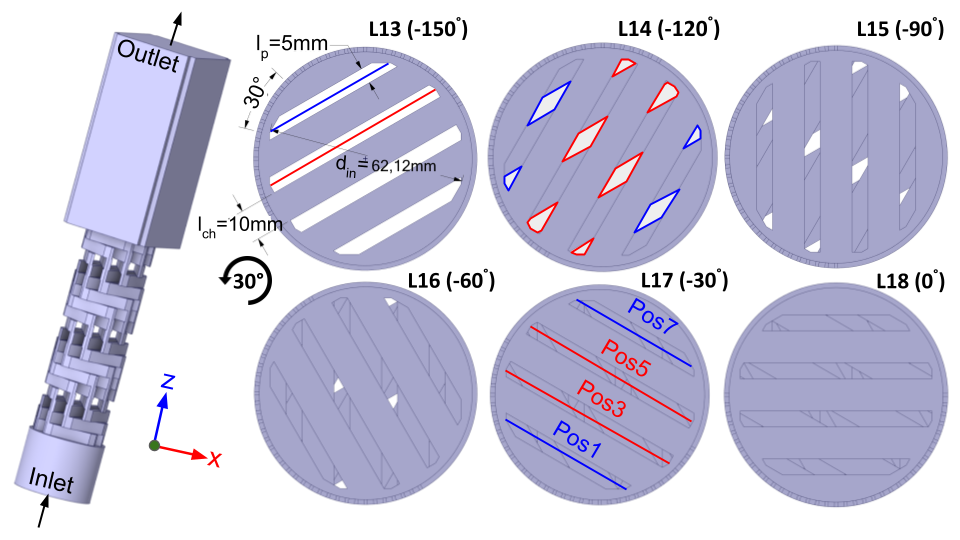
\includegraphics[width=0.95\linewidth]{images/geometry_description.png}
\caption{First column: Example geometry of a rotationally-stacked packed bed with a total of 18 layers L1 to L18 (reprinted from~\cite{velten2026}). The surrounding cylindrical wall containing the flow is not shown to reveal the internal structure of the topology. Right: (top-left corner) Single element; then (from left to right and top to bottom), successively stacked beds involving one, two\ldots six layers (L13 showing only the first layer, L18 all six layers tightly stacked on top of each other), with a constant rotation angle $\theta=30^\circ$ between two successive layers in the present case. The white regions shown in L13 to L16 indicate line-of-sight channels connecting directly inlet of the first element to outlet of the last element in a straight way; in the present case, such channels completely disappear after reaching L17, i.e., when stacking five elements on each other. The blue and red lines indicate the locations considered for PIV measurements in each layer and later comparisons, with labels (Pos1, Pos3, Pos5, Pos7) in each layer. The regions delimited by blue or red lines shown for L14 correspond to straight through-passages connecting a lower module to the one above it~\cite{velten2026}. For $\theta=30^\circ$, 2 such passages are found at positions Pos1 and Pos7 (white regions delimited by a blue boundary), and 3 passages at positions Pos3 and Pos5 (red boundary).}
\label{fig:geometry}
\end{figure}

Several identical elements are then stacked tightly on top of each other in vertical direction, each element being rotated by a certain angle (identical or not) compared to the previous element in the pile. Parameter $\theta_{i}$ is the angle between layer L$i$ and its top-side neighbour, layer L($i$+1); whenever this angle is constant, it will be written $\theta$, without any index. A total number $N$ of elements is stacked together, starting with element L1 and finishing with element L$N$. By stacking the elements on top of each other, a packing is finally obtained. The exact geometrical features of the packing depend on the rotation angle(s) $\theta_{i}$ between the elements. We will often use in what follows the concept of ``topology'' to denote the resulting, overall geometry of the packing.

The complex inlet section of the experimental setup, which was designed to ensure a fully homogeneous flow enters the first layer of the packing, was not included in the computational domain. Instead, a uniform inlet of the same circular cross-section (shown as `inlet' in Fig.~\ref{fig:geometry}, left), extended upstream by a short straight section ($60\,\mathrm{mm}$) sufficient for the velocity profile to homogenise before it reaches the first module.

%The bed is bounded by a gas inlet zone - a diffuser filled with $3\,\mathrm{mm}$ glass beads followed by a tranquilisation zone that distributes the flow homogeneously over the circular cross-section $A = 3031\,\mathrm{mm^2}$ - and, on top of the $18$th layer, a rectangular optical outlet box ($70\times70\,\mathrm{mm^2}$
%windows, height $200\,\mathrm{mm}$) that minimises the influence of the surroundings on the bed-surface flow~\cite{velten2026}.
%In the present work do not resolve this inlet with so many extra diffusor parts. Instead, the diffuser and tranquilisation zone are replaced by a uniform inlet of the same circular cross-section as the bed, extended upstream by a short straight section ($60\,\mathrm{mm}$) sufficient for the velocity profile to homogenise before it reaches the first module.
This reproduces the experimentally intended uniform feed while avoiding the high cost of meshing a diffuser filled with small glass beads, substantially reducing complexity and node count of the computational domain.

After leaving the packed bed, the airflow enters an empty rectangular container before escaping into the surrounding atmosphere, as in the experiments.

%\subsection{Rotationally Periodic Packing}
%\label{sec:geometry:topology}
Since the modules are identical and only their angular orientation changes, the bed topology is fully controlled by rotation, leading in some cases to rotational periodicity. Each layer L($i$+1) is the same as the one below it, L$i$, rotated about the column axis by the angle $\theta_i$ and shifted up by one layer height $l_\mathrm{h}$. The structure therefore possesses three characteristic geometrical features that can be changed (keeping the geometry of one element fixed). The first is the rotation angle $\theta_i$ between layer L$i$ and L($i$+1), which controls how far the gaps (and hence possible through-flowing gas jets) stay aligned before they are finally occluded by the bars of a following module. The second is the layer height $l_\mathrm{h}=10\,\mathrm{mm}$; since this parameter has never been changed during the present study, it will not be discussed further. Last but far more important is the superlattice period - only defined in cases where rotational periodicity is found, whenever the stack returns exactly to its original angular position after a certain number of rotations.

A consequence of the $180^\circ$ symmetry of the elements is that the inner pore network is point-symmetric between two successive layers: the first and fourth gaps (Pos1 and Pos7 shown in Fig.~\ref{fig:geometry}, third column) carry the same number of straight channels crossing both elements, and this applies as well to the second and third gaps (Pos3 and Pos5). Depending on $\theta$, between one and four straight through-passages connect a lower module to the one above it~\cite{velten2026}. For $\theta=30^\circ$ (see Fig.~\ref{fig:geometry}, third column, element L14), 2 such passages are found at positions Pos1 and Pos7 (white regions delimited by a blue boundary), and 3 passages at positions Pos3 and Pos5 (red boundary). Again, these passages exist only between two successive elements, and are rotated to other angular positions when further modules are added. For $\theta=30^\circ$ (Fig.~\ref{fig:geometry}), no straight through-passage exists when stacking at least five elements on top of each other.

In all other configurations, the porosity of the stack is still that of the individual element, since the rotation only redistributes the same solid volume within each layer; what changes with the value(s) of $\theta_i$ is the connectivity of the pore network, i.e., how the gaps of successive layers overlap.

In particular, when a constant rotation angle $\theta$ brings the stack back to an identical orientation after a finite number of layers, the overall topology becomes geometrically periodic: the geometry repeats after six layers for $\theta=30^\circ$ and after nine layers for $\theta=40^\circ$. In that case, the flow channels trace roughly a step-by-step spiral path through the bed (look again at the left part of Fig.~\ref{fig:geometry}). Finally, when $\theta_i$ is not constant and involves arbitrary values, the resulting aperiodic, irregularly rotated stack provides a geometrically disordered topology.

For the case $\theta=30^\circ$ (shown in Fig.~\ref{fig:geometry}), exactly the same geometry repeats every six layers: the block L1-L6 is identical to L7-L12 and to L13-L18, so that indeed three identical beds are stacked on top of each other to produce the overall topology, with a superlattice period $6 l_\mathrm{h}$.

For $\theta = 40^\circ$ the superlattice period is $9 l_\mathrm{h}$ and the bed with a total of 18 layers contains two identical parts.

\added{It should be noted that, for any constant rotation angle $\theta$, the stack possesses an additional symmetry: it is invariant under a rotation by $\theta$ about the column axis combined with a shift by one layer height $l_\mathrm{h}$ (screw symmetry). This holds independently of whether $180^\circ/\theta$ is an integer. Consequently, apart from the inlet and outlet regions, every layer has exactly the same neighbourhood once its rotation is removed. It is this property, rather than the superlattice period, that is probed by the layer-to-layer comparisons of Sec.~\ref{sec:locking}; an irregular sequence of angles breaks it.}\remark{1}{Central point. The locking metric compares single layers, so the observed recurrence follows from the constant rotation angle (screw symmetry), not from the 6- or 9-layer period. ``Rotational periodicity'' was therefore replaced by ``constant rotation angle'' in the abstract, introduction, Sec.~\ref{sec:locking} and the Conclusions.}

The comparisons with optical measurements will take place for layers L13-L17, close to the end of the bed, where the flow has been found experimentally to be fully developed~\cite{velten2026}. The simulations, by contrast, resolve of course all layers within the bed (as well as the additional inlet and outlet regions). Layers L1-L2 will be excluded from the analysis to allow the inlet flow to establish and develop within the bed (L03 is still shown in some figures to illustrate this development). Similarly, the last layer L18 is not considered because the flow escapes to a free space immediately above it and becomes sensitive to any outside perturbations. While 2D-PIV can only determine two velocity components in a limited set of measurement planes, the experimentally validated simulation removes this limitation by reconstructing the complete three-dimensional pore-scale velocity field throughout the bed, granting access to all layers, positions, and interstitial regions that are inaccessible to measurements. This capability allows the layer-to-layer organisation of the flow within the porous structure to be interrogated in full across all layers using LBM.

%\subsection{Topology Configurations}
%\label{sec:geometry:topologies}

%The modularity of the reactor allows a continuum of pore structures to be assembledfrom the same hardware simply by choosing the inter-layer rotation angle~\cite{velten2026}.
In order to derive generally-valid statements, three different packing topologies are considered in the analysis. The first one involves rotational periodicity, with $\theta=30^\circ$, so that the geometry repeats itself after six elements. As shown in Fig.~\ref{fig:geometry} this case involves long, straight channels in flow direction. This case is used first for validation purposes (Sec.~\ref{sec:validation:surface}), since the comparison at the freeboard is performed for it.
The second topology is also periodic: for $\theta=40^\circ$, the geometry repeats in an identical manner after nine elements.
Finally, a fully irregular configuration with arbitrarily varying values of $\theta_i$ is investigated. Here, successive layers are rotated by a non-repeating sequence of angles, so there is no geometric periodicity rule and no superlattice period. \added{The sequence of angles used here is $\theta_i = [\ldots]$ ($i=1,\ldots,17$).}\remark{2}{Please insert the sequence of angles $\theta_i$ (needed for the in-plane transformation and for reproducibility).} This packing serves for comparisons: it shares the same bars, slits, porosity and bounding apparatus as the periodic cases but does not repeat itself and is, therefore, not expected to exhibit any flow locking.


%Simulations at Re$_p = 100$ and Re$_p = 300$ are performed for all three packing topologies ($30^\circ$, $40^\circ$, and the irregular configuration), as corresponding PIV measurements are available for these conditions and provide the primary validation cases (Sec.~\ref{sec:validation}).


\subsection{Measurement Positions and Coordinate System}
\label{sec:geometry:coords}
A right-handed global Cartesian system $(x,y,z)$ is fixed to the apparatus: $x$ is horizontal, the depth axis $y$ originates at the centre of the module and is oriented parallel to the orientation of the bars of the topmost module, and the streamwise axis $z$ points upward with its origin at the bottom of the lowest module (see Fig. ~\ref{fig:geometry} and ~\ref{fig:coords}). Since each measurement plane lies in a void at a different rotation angle, a second, in-plane coordinate system $(x',y',z)$ is used in addition. It keeps the same vertical axis $z$, but its horizontal axis $x'$ is aligned with the direction of the open slit of the respective plane and is zero at the void centre. The global system is used for the apparatus geometry and for the positions of the measurement planes (Figs.~\ref{fig:geometry} and~\ref{fig:coords}), whereas the in-plane system is used for all velocity fields, axis labels and error metrics of the results (Sec.~\ref{sec:validation} onwards). The two directly reported velocity components are the horizontal in-plane velocity $v_{x'}$ and the vertical (streamwise) velocity $v_z$, since these correspond to the measured velocity components using planar PIV.\\
A vertical measurement plane is located in the global reference frame by its offset $a_{\mathrm{Pos},n}$ from the reactor centre (with $n=1,3,5,7$ the position number), measured along $y$ for the $0^\circ$ orientation of the module; this offset is independent of the rotation angle. Four positions are defined (Table~\ref{tab:pos}), as has already been shown in Fig.~\ref{fig:geometry}. Because the bed is point-symmetric about the column axis, Pos1/Pos7 and Pos3/Pos5 form point-symmetric pairs; the experiment exploits this symmetry, measuring only at Pos1 and Pos3 to recover the full set of flow fields~\cite{velten2026}. The present validation correspondingly extracts simulation planes at Pos1 and Pos3 as well.

%Because the gap in which each plane lies has been rotated depending on the layer in which it is placed (as discussed in Sec.~\ref{sec:geometry}), the raw simulation results are first de-rotated into a common in-plane frame before any further comparison or layer-to-layer analysis. Hence, each layer L$i$ is de-rotated about the central vertical axis in order to get an orientation corresponding to that of layer L18, chosen as a reference. The de-rotation angle prescribed to each lower layer L$i$ (with $i<18$) is therefore given by
%\begin{equation}
%    \alpha_i = \sum_{j=i}^{17}\theta_j.
%    \label{eq:derotation}
%\end{equation}
%In that manner, the open slits of every layer are aligned after de-rotation with those of element L18, so that they all appear along the in-plane axis $\xi$.
Each measurement plane is expressed in the in-plane system of its own layer: the global coordinates $(x,y,z)$ are rotated about the column axis by the angle $\alpha_i$ of layer L$i$ relative to the reference layer L18, so that the open slit lies along $x'$:\remark{3}{The definition of $\alpha_i$ (formerly $\alpha_i=\sum_{j=i}^{17}\theta_j$, see the commented-out lines above) and the sign convention of $\theta_i$ are no longer given in the text. Please reinstate them.}
\begin{subequations}
\label{eq:transform}
\begin{align}
    x' &= x\cos\alpha_i - y\sin\alpha_i, \\
    y' &= x\sin\alpha_i + y\cos\alpha_i,
\end{align}
\end{subequations}
and the velocity components $(v_x, v_y, v_z)$ are rotated consistently,
\begin{subequations}
\label{eq:transform_vel}
\begin{align}
    v_{x'} &= v_x\cos\alpha_i - v_y\sin\alpha_i, \\
    v_y' &= v_x\sin\alpha_i + v_y\cos\alpha_i,
\end{align}
\end{subequations}
with the vertical coordinate and the streamwise velocity left unchanged. The later reported in-plane velocity magnitude combines only the measured horizontal in-plane and streamwise components within the plane,
\begin{equation}
    |V| = \sqrt{ {v_{x'}}^2 + {v_z}^2 },
    \label{eq:velmag}
\end{equation}
keeping in mind that the third component, $v_y'$, is not measured experimentally and, therefore, does not enter the comparison.
After this transformation, $v_{x'}$ and $v_z$ are the in-plane components that can be compared directly with planar PIV.
\begin{table}[tbp]
\caption{Distance $a_{\mathrm{Pos},n}$ from the reactor centre to each measurement
position \cite{velten2026}.}
\label{tab:pos}
\begin{tabular}{lcccc}
\hline\noalign{\smallskip}
Pos. & 1 & 3 & 5 & 7 \\
\noalign{\smallskip}\hline\noalign{\smallskip}
$a_{\mathrm{Pos},n}$ (mm) & $-22.5$ & $-7.5$ & $7.5$ & $22.5$ \\
\noalign{\smallskip}\hline
\end{tabular}
\end{table}

\begin{figure}[tbp]
\centering
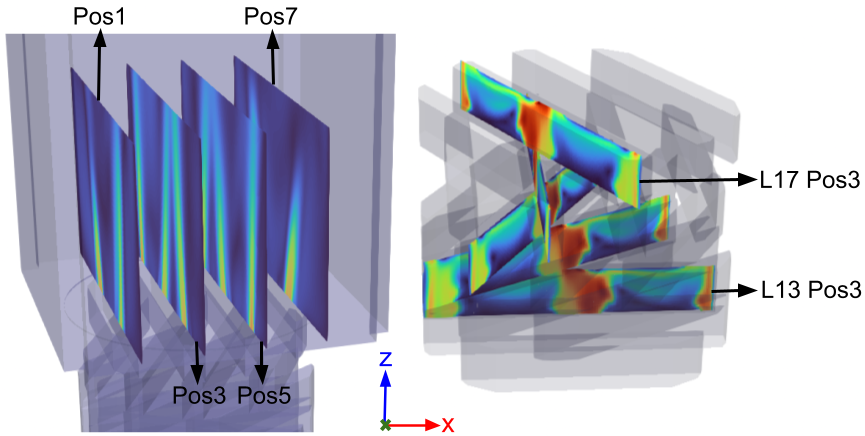
\includegraphics[width=0.95\linewidth]{images/geo_illustration.png}
\caption{Measurement positions and coordinate system for the rotationally stacked packed bed. Left: Schematic showing the four measurement positions (Pos1, Pos3, Pos5, Pos7) above the porous structure, illustrating their spatial arrangement and point-symmetric pairs (Pos1/Pos7 and Pos3/Pos5, see also Fig.~\ref{fig:geometry}). Right: Example velocity-magnitude fields $|V|$ obtained numerically in layers L13 to L17 at position Pos3, demonstrating the layer-resolved flow field extraction used for validation against PIV measurements before transformation into the in-plane system.}
\label{fig:coords}
\end{figure}

\section{Numerical Methods}
\label{sec:numerics}
First, the employed LBM algorithm is presented. It relies on enhanced central moments to efficiently satisfy momentum balance for incompressible flows~\cite{hosseini2022lattice}. Subsequently, the flow-locking analysis used to quantify the recurrence of pore-scale flow structures between successive packing layers is described.
\subsection{Lattice Boltzmann Formulation}
\label{sec:numerics:lbm}

The flow simulations presented here are performed using the lattice Boltzmann method (LBM), as it is implemented in our in-house code, ALBORZ. LBM may be regarded as a discretisation on the kinetic scale of the Boltzmann equation that recovers the Navier-Stokes equations in the hydrodynamic limit~\cite{Xiaoyi}. The numerical solver and formulation adopted here are identical to those previously developed and validated against experiments in a body-centred cubic (BCC) packing of spheres in our previous work~\cite{neeraj2023}; readers are referred to that work for a comprehensive description. Briefly, the method begins with a projection of the Boltzmann equation onto a discrete velocity space, whereby the particle distribution function is approximated through a truncated Hermite polynomial expansion. Integration of the resulting system of coupled hyperbolic equations along their characteristic trajectories~\cite{Bhadauria} yields the well-known two-step stream-and-collide algorithm:
\begin{equation}
    f_i\left(\bm{r}+\bm{c}_idt, t+dt\right) - f_i\left(\bm{r}, t\right) = \Omega_i.
\end{equation}
Here, $f_i$ denotes the discrete populations advected along the lattice links with velocities $\bm{c}_i$, $dt$ is the discrete time increment, and $\Omega_i$ is the collision operator, which drives the populations towards their equilibrium state in mimicry of inter-molecular collisions. For weakly non-equilibrium flows, i.e., at the low Knudsen numbers characteristic of the present configuration, it is common to adopt first the single-relaxation-time Bhatnagar-Gross-Krook (BGK) closure, whose discrete counterpart reads:
\begin{equation}
    \Omega_i = \omega\left( f^{\rm eq}_i - f_i\right) + \Xi_i,
\end{equation}
in which $\omega$ sets the rate of relaxation towards equilibrium and $f^{\rm eq}_i$ is the discretised equilibrium attractor, i.e., the Maxwell-Boltzmann distribution recovered as the entropy-\deleted{minimising}\added{maximising} state~\cite{Bhadauria,Shu}. The additional term $\Xi_i$ is a correction that compensates for the spurious deviations arising in the diagonal entries of the third-order equilibrium moments whenever a third-order quadrature is used. The equilibrium itself is constructed, as is standard in the method, by truncating the Hermite expansion of the Maxwell-Boltzmann distribution at finite order and evaluating it on the Gauss-Hermite quadrature nodes:
\begin{equation}
    f^{\rm eq}_i = w_i \sum_{n=0}^{\deleted{N}\added{N_\mathcal{H}}}\frac{1}{n!c_s^{2n}} \mathcal{H}^n(\bm{c}_i):a_n^{\rm eq}(\rho,\bm{u},p/\rho),
\end{equation}
where $\mathcal{H}^n$ denotes the rank-$n$ Hermite polynomial tensor, $a_n^{\rm eq}$ its associated equilibrium coefficient, $w_i$ the quadrature weights and $c_s$ the lattice sound speed fixed by the quadrature; $\rho$, $\bm{u}$ and $p$ are the density, velocity and pressure, and $\deleted{N}\added{N_\mathcal{H}}$ the truncation order. Throughout this work we employ the D3Q27 lattice (with $D$ the spatial dimension, $Q$ the number of links), which corresponds to a third-order quadrature; the expansion is therefore truncated at $\deleted{N}\added{N_\mathcal{H}}=6$ in three dimensions, this being the highest orders the respective stencils can support. A virtue of this higher-order construction, in contrast with the conventional second-order equilibrium, is that the shear-mode dissipation rate retains Galilean invariance at the Navier-Stokes level. The complementary correction $\Xi_i$ extends this invariance to the dissipation of the normal modes and is given by~\cite{hosseini2020compressibility,feng2015three}\added{,~\cite{hosseini2022consistent,hosseini2024combustion}}:
\begin{equation}\label{eq:correction}
    \Xi_i = \left(1-\frac{\omega}{2}\right)\added{dt\,}\frac{w_i}{2c_s^4}\deleted{\left(\bm{\nabla}\mathcal{H}^2\right):\Delta^{\rm eq}_3}\added{\mathcal{H}^2(\bm{c}_i):\left(\bm{\nabla}\cdot\Delta^{\rm eq}_3\right)
    = \left(1-\frac{\omega}{2}\right)dt\,\frac{w_i}{2c_s^4}\sum_{\alpha}\mathcal{H}^2_{\alpha\alpha}(\bm{c}_i)\,\partial_\alpha\Delta^{\rm eq}_{\alpha\alpha\alpha}},
\end{equation}
with $\Delta^{\rm eq}_3$ the rank-three diagonal tensor
\begin{equation}
    \Delta^{\rm eq}_{\alpha\alpha\alpha} = \rho u_\alpha \left(u_\alpha^2 + 3p/\rho\right) - \sum_i c_{i,\alpha}^3 f^{\rm eq}_i\added{ = \rho u_\alpha \left(u_\alpha^2 + 3p/\rho - 3c_s^2\right)},
\end{equation}
\added{where the last equality uses $c_{i,\alpha}^3 = 3c_s^2\,c_{i,\alpha}$ on the D3Q27 lattice. Note that the spatial derivative acts on the deviation tensor, the Hermite polynomial depending only on $\bm{c}_i$.}\remark{5}{In the original form, the gradient acted on $\mathcal{H}^2$, which depends only on $\bm{c}_i$, and the double contraction of two rank-3 tensors gave a vector. Corrected form following Refs.~\cite{hosseini2022consistent,hosseini2024combustion}. The same error is present in Eqs.~(4) and (13) of Ref.~\cite{neeraj2023}.}\remark{6}{The expression for $\Delta^{\rm eq}_{\alpha\alpha\alpha}$ was correct; the equality is only added for clarity.}
In practice the plain BGK operator is frequently replaced by more elaborate collision models, motivated either physically (e.g., to recover an arbitrary Prandtl number) or numerically (to enhance stability). A prominent example is the multiple-relaxation-time (MRT) approach, in which the relaxation is performed not on the populations themselves but on a set of independent base-functions (usually moments of the distribution), which has gained wide adoption thanks to its favourable stability and accuracy. The collision model used in this study is an MRT operator formulated in a basis of modified central Hermite moments, which in particular permits the bulk viscosity to be tuned independently~\cite{hosseini2022lattice}. Unlike the classical Hermite-moment basis~\cite{hosseini2021central,huang2022simulation}, this choice lets the trace and the deviatoric parts of the second-order moments relax with distinct rates:
\begin{equation}
    \Omega_i = \mathcal{T}^{-1}W\mathcal{T}(f^{\rm eq}_i - f_i) + \Xi_i\label{eq:correc1}
\end{equation}
where $\mathcal{T}$ maps the populations into moment space, $\mathcal{T}^{-1}$ is its inverse and $W$ collects the relaxation rates on its diagonal. The transform $\mathcal{T}$ is built from the modified central Hermite polynomials $\widetilde{\mathcal{H}}^n(\bm{c}_i)$. This tensor is defined based on a set of Hermite polynomials which are expressed as follows:
\begin{equation}
\begin{matrix}
 \mathcal{H} = \{\mathcal{H}_0^{(0)}, \mathcal{H}_x^{(1)}, \mathcal{H}_y^{(1)}, \mathcal{H}_z^{(1)}, \mathcal{H}_{xy}^{(2)}, \mathcal{H}_{xz}^{(2)}, \mathcal{H}_{yz}^{(2)}, \mathcal{H}_{x^2}^{(2)}-\mathcal{H}_{y^2}^{(2)}, \mathcal{H}_{x^2}^{(2)}-\mathcal{H}_{z^2}^{(2)},\mathcal{H}_{x^2}^{(2)}+\\\mathcal{H}_{y^2}^{(2)} +\mathcal{H}_{z^2}^{(2)}, \mathcal{H}_{x^2y}^{(3)},
 \mathcal{H}_{x^2z}^{(3)},\mathcal{H}_{xy^2}^{(3)},\mathcal{H}_{y^2z}^{(3)}, \mathcal{H}_{xz^2}^{(3)},\mathcal{H}_{yz^2}^{(3)},
\mathcal{H}_{xyz}^{(3)}, \mathcal{H}_{x^2y^2}^{(4)}, \mathcal{H}_{x^2z^2}^{(4)}, \mathcal{H}_{y^2z^2}^{(4)},\\  \mathcal{H}_{x^2yz}^{(4)},  \mathcal{H}_{xy^2z}^{(4)}, \mathcal{H}_{xyz^2}^{(4)},\mathcal{H}_{x^2y^2z}^{(5)},  \mathcal{H}_{x^2yz^2}^{(5)}, \mathcal{H}_{xy^2z^2}^{(5)}, \mathcal{H}_{x^2y^2z^2}^{(6)} \}.
\end{matrix}
\label{Eq:LBM-3dh}
\end{equation}
% which for the D2Q9 lattice take the form:
% \begin{subequations}
% 	\begin{align}
% 	\widetilde{\mathcal{H}}_0 &= 1, \\
% 	\widetilde{\mathcal{H}}_x &= c_{i,x}-u_x, \\
% 	\widetilde{\mathcal{H}}_y &= c_{i,y}-u_y, \\
% 	\widetilde{\mathcal{H}}_{xy} &= (c_{i,x}-u_x) (c_{i,y}-u_y), \\
% 	\widetilde{\mathcal{H}}_{xx-yy} &= {(c_{i,x}-u_x)}^2 - {(c_{i,y}-u_y)}^2, \\
% 	\widetilde{\mathcal{H}}_{xx+yy} &= {(c_{i,x}-u_x)}^2 + {(c_{i,y}-u_y)}^2 - 2c_s^2,\\
% 	\widetilde{\mathcal{H}}_{xxy} &= {(c_{i,x}-u_x)}^2(c_{i,y}-u_y) - c_s^2(c_{i,y}-u_y),\\
% 	\widetilde{\mathcal{H}}_{xyy} &= {(c_{i,y}-u_y)}^2(c_{i,x}-u_x) - c_s^2(c_{i,x}-u_x),\\
% 	\widetilde{\mathcal{H}}_{xxyy} &= \left[{(c_{i,x}-u_x)}^2 - c_s^2\right] \left[{(c_{i,y}-u_y)}^2 - c_s^2\right].
% 	\end{align}
% \end{subequations}
%%
%Projecting the equilibrium onto this basis yields the corresponding central Hermite coefficients $\widetilde{a}^{\rm eq}_n$, which for the D2Q9 equilibrium are:
%\begin{subequations}
%	\begin{align}
%	\widetilde{a}^{\rm eq}_0 &= \rho, \\
%	\widetilde{a}^{\rm eq}_x &= 0, \\
%	\widetilde{a}^{\rm eq}_y &= 0, \\
%	\widetilde{a}^{\rm eq}_{xy} &= 0, \\
%	\widetilde{a}^{\rm eq}_{xx-yy} &= 0, \\
%	\widetilde{a}^{\rm eq}_{xx+yy} &= 2(p - \rho c_s^2),\\
%	\widetilde{a}^{\rm eq}_{xxy} &= 0,\\
%	\widetilde{a}^{\rm eq}_{xyy} &= 0,\\
	%\widetilde{a}^{\rm eq}_{xxyy} &= \rho{(p/\rho - c_s^2)}^2.
%	\end{align}
%\end{subequations}
%For the particular choice $p=\rho c_s^2$ every coefficient above vanishes except the zeroth-order one.
On the D3Q27 lattice the diagonal relaxation tensor $W$ is assembled as:
\begin{equation}
    W={\rm diag}(1,1,1,1,\omega_{s},\omega_{s},\omega_{s},\omega_{s},\omega_{s},\omega_{b},\omega_{a},...,\omega_{a}),
\end{equation}
where the operator ${\rm diag}$ is defined as:
\begin{equation}
    {\rm diag}(\bm{A}) = (\bm{A}\otimes\bm{1})\circ \bm{I},
\end{equation}
in which $\bm{A}$ is an arbitrary vector, $\bm{1}$ the all-ones vector, $\bm{I}$ the identity tensor and $\circ$ the Hadamard (element-wise) product. The entries $\omega_s$, $\omega_b$ and $\omega_a$ are the relaxation frequencies of the shear, bulk and ghost modes, respectively. The bulk-mode frequency $\omega_b$ is tied to the bulk viscosity $\eta$ through:
\begin{equation}
    \omega_b = \frac{dt}{\deleted{(\frac{2+D}{D}-\frac{\partial\ln p}{\partial\ln \rho})\frac{\eta}{p}}\added{\dfrac{\eta}{\left(\frac{2+D}{D}-\frac{\partial\ln p}{\partial\ln \rho}\right)p}} + dt/2}\added{,}
\end{equation}
\added{which follows from $\eta = \left(\frac{2+D}{D}-\frac{\partial\ln p}{\partial\ln \rho}\right)\left(\frac{1}{\omega_b}-\frac{1}{2}\right)dt\,p$~\cite{hosseini2022consistent}. For $\omega_b=\omega_s$ and $p=\rho c_s^2$ (i.e., $\partial\ln p/\partial\ln\rho=1$), this recovers the BGK value $\eta=\frac{2}{3}\mu$ in three dimensions. In the present simulations, $\omega_b=[\ldots]$ and $\omega_a=[\ldots]$ are used.}\remark{7}{Corrected relation for $\omega_b$ (the factor was on the wrong side). Please insert the values of $\omega_b$ (or $\eta$) and $\omega_a$ used.}
Within this multi-relaxation framework the third-order correction $\Xi_i$ of Eq.~\ref{eq:correction} is recast accordingly, the single frequency $\omega$ being replaced by the harmonic combination of the shear and bulk rates:
\begin{equation}\label{eq:correction_MRT}
    \Xi_i = \left(1-\frac{\omega_b\omega_s}{\omega_b+\omega_s}\right)\added{dt\,}\frac{w_i}{2c_s^4}\deleted{\left(\bm{\nabla}\mathcal{H}_2\right):\Delta^{\rm eq}_3}\added{\mathcal{H}^2(\bm{c}_i):\left(\bm{\nabla}\cdot\Delta^{\rm eq}_3\right)}.
\end{equation}
\remark{5}{Same correction as in Eq.~(\ref{eq:correction}). Please confirm the prefactor against Ref.~\cite{hosseini2022lattice}; it reduces correctly to $1-\omega/2$ for $\omega_b=\omega_s$.}
Taken together, the formulation outlined above delivers a freely adjustable bulk viscosity while preserving the Galilean invariance of both the dynamic and the bulk viscosities~\cite{hosseini2022lattice,hosseini2020compressibility}. Additionally, it shows very favourable stability bounds~\cite{hosseini2022lattice,neeraj2023}.

\subsection{Computational Domain and Boundary Conditions}
\label{sec:numerics:domain}

While a variety of different boundary conditions have been developed for the lattice Boltzmann method, in the context of the present study all solid boundaries are modelled using the half-way bounce-back scheme where missing populations after the collision-streaming steps are computed as~\cite{kruger2017lattice}:
\begin{equation}
    f_\alpha\left(\bm{x},t+dt\right) = f^{*}_{\bar{\alpha}}\left(\bm{x},t\right),
\end{equation}
where $f^{*}$ is the post-collision population (prior to streaming) and $\bar{\alpha}$ is the index of the particle velocity opposite that of $\alpha$. To get rid of the staircase approximation the half-way bounce-back is supplemented with the treatment for curved boundaries as proposed in~\mbox{\cite{bouzidi2001momentum}}.

Therefore, at any given \deleted{boundary node}\added{fluid node} $\bm{x}_f$\added{ adjacent to the wall}, the missing incoming populations are computed as:
\begin{subequations}
	\begin{align}
		f_\alpha(\bm{x}_f, t+dt) &= 2qf_{\bar{\alpha}}(\bm{x}_f+\bm{c}_{\bar{\alpha}}, t+dt)\nonumber \\  &+\left(1-2q\right)f_{\bar{\alpha}}(\bm{x}_f, t+dt), \quad \forall\; q<\frac{1}{2},\\
		f_\alpha(\bm{x}_f, t+dt) &= \frac{1}{2q}f_{\bar{\alpha}}(\bm{x}_f+\bm{c}_{\bar{\alpha}}, t+dt)\nonumber \\  &+\frac{2q-1}{2q}\deleted{f_{\bar{\alpha}}(\bm{x}_f, t+dt)}\added{f_{\alpha}(\bm{x}_f+\bm{c}_{\alpha}, t+dt)}, \quad \forall\; q\geq\frac{1}{2},
		\end{align}
	\label{Eq:CE_moments_eq}
\end{subequations}
where $\bar{\alpha}$ designates the direction opposite $\alpha$ and $q$ is computed as:
\begin{equation}
    q = \frac{\lvert\lvert \bm{x}_f - \bm{x}_s\lvert\lvert}{\lvert\lvert\bm{c}_\alpha \lvert\lvert},
\end{equation}
with $\bm{x}_s$ denoting the wall position in direction $\deleted{\alpha}\added{\bar{\alpha}}$. \added{Here, all populations on the right-hand side are post-streaming values: $f_{\bar{\alpha}}(\bm{x}_f+\bm{c}_{\bar{\alpha}}, t+dt)=f^*_{\bar{\alpha}}(\bm{x}_f,t)$ is the population that left $\bm{x}_f$ towards the wall (stored at the solid node), $f_{\bar{\alpha}}(\bm{x}_f, t+dt)=f^*_{\bar{\alpha}}(\bm{x}_f-\bm{c}_{\bar{\alpha}},t)$ the one arriving at $\bm{x}_f$ from the neighbouring fluid node, and $f_{\alpha}(\bm{x}_f+\bm{c}_{\alpha}, t+dt)=f^*_{\alpha}(\bm{x}_f,t)$ the one that left $\bm{x}_f$ in the direction opposite to the wall. Equation~(\ref{Eq:CE_moments_eq}) thus corresponds to Eqs.~(5a) and (5b) of Ref.~\cite{bouzidi2001momentum}, written in post-streaming form.}\remark{8}{The second term of the $q\ge 1/2$ case has been corrected: it must be the population that left $\bm{x}_f$ away from the wall (Bouzidi et al.: interpolation between the reflection point D and node E). Note also a misprint in Eq.~(5b) of Bouzidi et al.: $\bm{r}_i$ should read $\bm{r}_l$.}

Other boundary conditions applied at the inlets and outlets, i.e., constant velocity and constant pressure, are realised using the non-equilibrium extrapolation approach proposed in~\cite{zhao2002non}.
%In this approach the missing populations at the boundary nodes are reconstructed as:
%\begin{equation}
%%\end{equation}
%where $\bm{x}_w$ is the position of the boundary node and $f^{(neq)}$ the non-equilibrium part of the distribution function. One of the two variables (density or velocity) is known via the boundary condition and the other is computed by interpolation from neighboring nodes. The non-equilibrium part of the distribution function is also computed via an interpolation in space.

\subsection{Locking Order Parameter \texorpdfstring{$L(n)$}{L(n)}}
\label{sec:locking:Ln}

To quantify the similarity of flows at pore scale between different layers, we introduce here a flow-locking metric. Flow locking is defined as the recurrence of the same time-averaged flow after accounting for the geometric rotation between different elements. The similarity measure itself is based on the normalised spatial inner product widely used in velocity-field analysis or proper orthogonal decomposition (POD)~\cite{lumley1967,sirovich1987,berkooz1993pod}. The novelty of this approach, therefore, lies not in the mathematical formulation itself, but in its application to the analysis of pore-scale velocity fields in the in-plane system as an objective measure of topology-induced flow recurrence.

The similarity between the mean velocity fields in the in-plane system of layers $m$ and $n$ is computed as
\begin{equation}
L_{mn}
=
\frac{\langle\tilde{\bm{v}}_m,\tilde{\bm{v}}_n\rangle_{\Omega}}
{\|\tilde{\bm{v}}_m\|_{\Omega}
\|\tilde{\bm{v}}_n\|_{\Omega}},
\qquad
\langle\bm{a},\bm{b}\rangle_{\Omega}
=
\sum_{i\in\Omega}
\left(
a_{x',i} b_{x',i}
+
a_{z,i} b_{z,i}
\right),
\label{eq:Ln}
\end{equation}
where $\tilde{\bm{v}}_q=(\tilde v_{x'},\tilde v_z)_q$ is the time-averaged in-plane velocity field (two components) of a single layer $q$ on its measurement plane, in the in-plane system (see Sec.~\ref{sec:geometry:coords}), while $\|\bm a\|_\Omega=\sqrt{\langle\bm a,\bm a\rangle_\Omega}$ is the Euclidean norm, i.e., the root of the sum of the squared in-plane components over all fluid points (a sum, not an average), and $\Omega$ denotes the set of fluid points of the plane, which is the same for all layers because all elements have identical geometry. The normalisation removes the influence of velocity magnitude. In the present configuration, this is not really necessary, but later applications will consider thermal flows in which local changes in temperature will induce noticeable changes of density, and hence velocity.

The metric uses only the two in-plane velocity components, $v_{x'}$ and $v_z$ (see Sec.~\ref{sec:geometry:coords} and Fig.~\ref{fig:coords} for the coordinate system). This is intentional: planar PIV measures exactly these two components, so simulations and experiments can be analysed with the same procedure.

The indices $m$ and $n$ label the two layers being compared. $L_{mn}$ is a normalised inner product (cosine similarity), so $L_{mn}=1$ means that the velocity fields of layers $m$ and $n$ show exactly the same flow pattern, up to a constant scale factor. Smaller values mean larger differences in the pore-scale flow. \added{Note, however, that Eq.~(\ref{eq:Ln}) is not mean-subtracted. It would be a correlation coefficient in the strict sense if the mean velocity within each layer were zero. Here, all fields share a common upward through-flow, so that even structurally unrelated fields yield a clearly positive value of $L_{mn}$; the value expected for uncorrelated flow patterns is therefore not zero, which must be kept in mind when interpreting $L_{mn}$.}\remark{9}{Alternatively, the layer mean could be subtracted before computing $L_{mn}$.} Evaluating Eq.~(\ref{eq:Ln}) for all layer pairs gives the layer-to-layer locking matrix, which is symmetric and has $L_{mm}=1$ on its diagonal.

Two scalar quantities summarise the locking behaviour. The mean locking strength,
\begin{equation}
\overline{L}
=
\frac{2}{N_L(N_L-1)}
\sum_{m<n}
L_{mn},
\label{eq:Lbar}
\end{equation}
is the average similarity between all distinct layer pairs and provides a single measure of the overall strength of flow locking in the whole region. Here, $N_L$ is the number of layers included in the analysis, and the sum runs over all $N_L(N_L-1)/2$ distinct layer pairs $m<n$. Values of $\overline{L}$ approaching unity would indicate that the flow structures are nearly identical in all layers building the packing, whereas lower values correspond to progressively weaker locking.

The second quantity, the per-layer locking,
\begin{equation}
L(n)
=
\frac{\langle\tilde{\bm{v}}_n,\bar{\bm{v}}\rangle_{\Omega}}
{\|\tilde{\bm{v}}_n\|_{\Omega}
\|\bar{\bm{v}}\|_{\Omega}},
\qquad
\bar{\bm{v}}
=
\frac{1}{N_L}
\sum_{m=1}^{N_L}
\tilde{\bm{v}}_m,
\label{eq:Lofn}
\end{equation}
measures the similarity of each individual layer to the mean flow field. \added{Since $\bar{\bm{v}}$ includes layer $n$ itself, $L(n)$ is slightly biased upward, the more so the smaller $N_L$.} Unlike $\overline{L}$, which characterises the packing as a whole, $L(n)$ identifies local departures from the locked state and therefore highlights layers that deviate most strongly from the repeating flow pattern.

\section{Simulation Parameters}
\label{sec:numerics:params}

In this study, the working fluid is air at the temperature of $T = 20\,^\circ\mathrm{C}$ and the pressure of $p = 1\,\mathrm{atm}$ with a density of $\rho = 1.204\,\mathrm{kg/m^3}$, and a dynamic viscosity of $\mu = 1.822\times10^{-5}\,\mathrm{kg/(m\,s)}$. The operating conditions are characterised by the particle Reynolds number defined as
\begin{equation}
    \hbox{Re}_p = \frac{\rho\,v_s\,l_\mathrm{ch}}{\varphi\,\mu},
    \label{eq:rep}
\end{equation}
with $l_\mathrm{ch}=10\,\mathrm{mm}$ the characteristic length and $v_s$ the superficial velocity~\cite{velten2026}, obtained from the volumetric flow rate $Q$ via $Q = A\,v_s$, where $A = 3031\,\mathrm{mm^2}$ denotes the inlet cross-section of the reactor.

In this study two different particle Reynolds numbers of Re$_p=100$ and $300$ are considered. In the reference experiment Re$_p = 100$ corresponds to an air flow rate of $Q = 9.14\,\mathrm{L/min}$ and Re$_p = 300$ corresponds to $Q = 27.42\,\mathrm{L/min}$~\cite{velten2026}.

The lattice is uniform and Cartesian. The decisive geometric length scale for the grid is the $5\,\mathrm{mm}$ gap width $l_P$, which is common to all three topologies. The final resolution employs about $17$ nodes across each slit (and correspondingly $33$ across each $10\,\mathrm{mm}$ bar) at Re$_p = 100$, following the grid-sensitivity study described in Sec.~\ref{sec:numerics:grid}. The lattice spacing and time step are further refined as the Reynolds number increases, both to keep the near-wall shear layers resolved and to \deleted{maintain a low}\added{limit the increase of the} lattice Mach number. As a consequence, the gap is resolved by $33$ nodes at Re$_p = 300$. The bed cross-section $d_\mathrm{in} = 62.12\,\mathrm{mm}$ and the streamwise extent spans the $18$-module stack plus the upstream inlet section of 60~mm and a long rectangular outlet (Fig.~\ref{fig:geometry}). The non-dimensional relaxation time $\tau$ is set from the target kinematic viscosity at each operating point; the resulting per-case discretisation parameters are collected in~Table~\ref{tab:simparams}.

\added{The choice of $dx$ and $dt$ keeps the relaxation time at $\tau = 0.5301$, i.e., sufficiently far from the stability limit $\tau\to0.5$, while reproducing the kinematic viscosity of air. As a consequence, the lattice speed of sound, $c_s = dx/(\sqrt{3}\,dt)$, is reduced to about $2.9\,\mathrm{m/s}$ (Re$_p=100$) and $5.8\,\mathrm{m/s}$ (Re$_p=300$), giving maximum Mach numbers of about $0.16$ and $[0.24]$, respectively. Compressibility errors scale as $Ma^2$; under the diffusive scaling used in the grid study ($dt\propto dx^2$ at fixed $\tau$), $Ma$ decreases proportionally to $dx$, so that these errors are included in the grid-convergence assessment of Sec.~\ref{sec:numerics:grid}. Moreover, since the pressure is carried by the density in LBM, the pressure drop across the bed induces a density variation $\Delta\rho/\rho_0\approx\Delta p/(\rho c_s^2)$, which was checked to remain below $[\ldots]\,\%$.}\remark{10}{Please insert the actual peak velocity at Re$_p=300$.}\remark{11}{A rough estimate hints towards relatively large density variations. Please check the mean density and the mass flux at inlet vs.\ outlet and the mean velocity magnitude per layer (L03--L17), and insert $\Delta\rho/\rho_0$.}
\begin{table}[tbp]
\caption{Discretisation parameters used in the final simulations for the two Reynolds numbers. The grid is set by the resolution required at each Re$_p$; the same grid is used for all topologies sharing a given Re$_p$.}
\label{tab:simparams}
\begin{tabular}{lcc}
\hline\noalign{\smallskip}
 & Re$_p = 100$ & Re$_p = 300$ \\
\noalign{\smallskip}\hline\noalign{\smallskip}
Grid $N_x\times N_y\times N_z$      & $273\times273\times1439$ & $539\times539\times2870$ \\
Total nodes                          & $1.07\times10^{8}$       & $8.34\times10^{8}$       \\
$dx$ (mm)                      & $0.30$                   & $0.15$                   \\
$dt$ (s)                       & $5.967\times10^{-5}$     & $1.492\times10^{-5}$     \\
$\tau$                               & $0.5301$                 & $0.5301$                 \\
Nodes per gap width ($l_P = 5\,$mm)       & $\approx17$              & $33$                     \\
\noalign{\smallskip}\hline
\end{tabular}
\end{table}

LBM simulations being intrinsically time-dependent, each case is advanced until it reaches a statistically stationary state, monitored through the $L_2$ norm of the velocity field between successive time steps; the run is
considered converged once this \added{[relative]} residual has dropped below $10^{-5}$, which was found to be obtained around $t = 10\,\mathrm{s}$ of physical time. Mean fields are then accumulated at every time step (with a constant sampling interval $dt$) over a window of 100 s. All velocity fields reported later are corresponding, time-averaged fields.\remark{12}{A residual between successive time steps is a steady-state criterion; with low-frequency pulsations and $dt\sim10^{-5}$\,s it is almost automatically met. Is it relative? Alternatively, use the convergence of the running mean.} Note that this long averaging time has been found necessary due to low-frequency pulsations observed in the bed both experimentally and numerically. All computations are carried out on the \emph{Sofja} cluster of the Otto von Guericke University Magdeburg using domain decomposition over $416$ nodes.

Finally, the two operating points in terms of Re$_p$ are combined with the three topologies of Sec.~\ref{sec:geometry}, leading to six cases.

\section{Results and Discussion}
\label{sec:results}
This section presents a systematic assessment of the numerical framework in three stages. First, a grid-sensitivity study is performed to establish the spatial resolution required for accurate predictions, followed by symmetry and consistency verification to further assess the reliability and robustness of the numerical approach. Second, the capability of the developed numerical tools to resolve flow behaviour within the packing structures is demonstrated through validation against the experimental measurements. Finally, a flow-locking analysis is conducted to investigate whether the pore network geometry induces repeatable flow patterns and to examine the influence of Reynolds number and topology on the persistence and evolution of these structures.

\subsection{Grid Sensitivity Study}
\label{sec:numerics:grid}
To determine an appropriate grid resolution, spatial convergence was first assessed at Re$_p = 100$ on a representative subdomain of the regular packing with $\theta=40^\circ$, shown in Fig.~\ref{fig:grid}. Extracting a part of the full bed enables the systematic comparison of several grid resolutions while maintaining a moderate computational cost.
The decisive geometric length scale is the $5\,\mathrm{mm}$ passage (or gap) width $l_P$, which is common to all three topologies and represents the smallest flow channel that must be resolved by the grid. Accordingly, the grid resolution is reported as the number of lattice nodes spanning one gap width. Three uniform grids - coarse, medium and fine - were considered, with their respective spacings $dx$, time steps $dt$ and total node counts summarised in Table~\ref{tab:grid}. The finest grid resolves each slit with $33$ nodes, the coarsest with $12.5$.
The relaxation time is held at $\tau = 0.5301$ across all three levels.
\begin{table}[tbp]
\caption{Discretisation levels used in the grid-sensitivity study, performed on a representative subdomain of the $40^\circ$ packing. Resolution is quoted as the number of lattice nodes across the $5\,\mathrm{mm}$ gap. Peak and mean velocity magnitudes are evaluated on the extraction surface of Fig.~\ref{fig:grid} (mean taken after interpolation onto a common $0.15\,\mathrm{mm}$ grid); errors are relative to the fine grid.}
\label{tab:grid}

\begin{tabular}{lccc}
\hline\noalign{\smallskip}
 & Coarse & Medium & Fine \\
\noalign{\smallskip}\hline\noalign{\smallskip}
$dx$ (mm)                  & $0.40$               & $0.30$               & $0.15$ \\
$dt$ (s)                   & $1.06\times10^{-4}$  & $5.97\times10^{-5}$  & $1.49\times10^{-5}$ \\
Grid $N_x\times N_y\times N_z$   & $206\times206\times393$ & $273\times273\times522$ & $539\times539\times1037$ \\
Nodes per slit                   & $12.5$               & $16.7$               & $33.3$ \\
$\tau$                           & $0.5301$             & $0.5301$             & $0.5301$ \\
\noalign{\smallskip}\hline\noalign{\smallskip}
Peak $|V|$ (m/s)            & $0.523$              & $0.464$              & $0.462$ \\
Error in peak (\%)               & $13.2$               & $0.5$                & Ref. \\
Mean $|V|$ (m/s)            & $0.0771$             & $0.0749$             & $0.0729$ \\
Error in mean (\%)               & $5.7$                & $2.7$                & Ref. \\
\noalign{\smallskip}\hline
\end{tabular}
\end{table}

Fig.~\ref{fig:grid} compares the time-averaged velocity-magnitude fields on the same extraction surface for the three grid resolutions. All grids reproduce the characteristic three-jet structure emerging from the slits, although the coarse grid yields slightly more diffuse jets and a noticeably higher peak velocity. In contrast, the medium and fine grids are nearly indistinguishable. The peak jet velocity differs by $13\%$ between the coarse and fine grids but by only $0.5\%$ between the medium and fine grids, while the mean velocity of the extracted surface differs by $2.7\%$ between the latter two (Table~\ref{tab:grid}). Using the mean velocity, the Grid Convergence Index~\cite{celik2008} is $0.9\%$ on the fine grid, with an observed order of convergence of $\deleted{2.2}\added{2.1}$\remark{13}{Sec.~\ref{sec:validation:surface} quotes $p\approx2.1$. My recalculation (Celik et al., unequal refinement ratios $2$ and $4/3$, mean velocities of Table~\ref{tab:grid}) gives $p\approx2.14$ and GCI $\approx1.0\%$. Please check and use one value consistently.}, corresponding well to the second order formally expected in space for LBM. Keeping in mind the very long simulation times needed to average over 100 s of physical time, a sufficient accuracy is considered achieved at medium resolution, which was adopted for all Re$_p=100$ simulations. This grid requires roughly one eighth of the nodes of the fine grid and, owing also to its larger time step, reduces computational cost by more than an order of magnitude while maintaining satisfactory agreement in both peak and mean velocities. However, the cases at higher Reynolds number (Re$_p=300$) have been simulated using the resolution of the fine grid (Table~\ref{tab:simparams}) to adequately resolve the thinner shear layers induced by higher velocities. For all cases, the number of points in streamwise direction has been of course correspondingly increased to include the full bed geometry (see again Table~\ref{tab:simparams}).

\begin{figure}[tbp]
\centering
\begin{subfigure}[b]{0.4\textwidth}
    \centering
    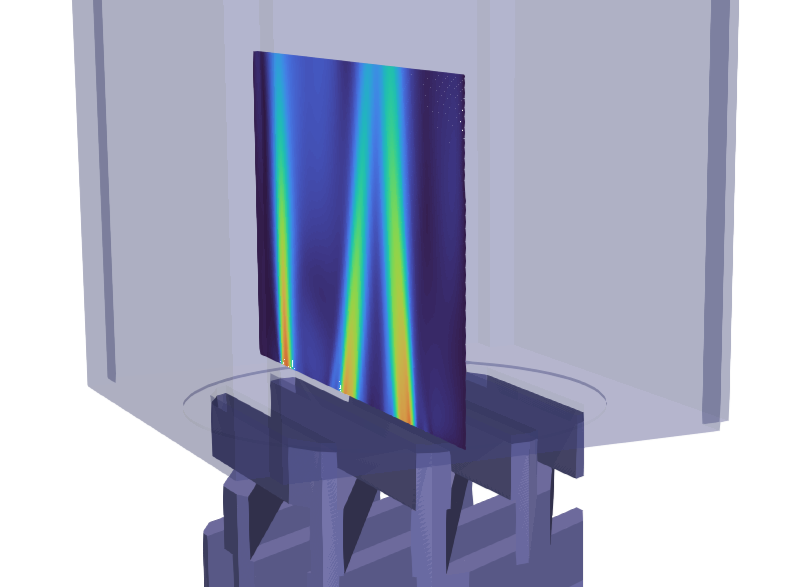
\includegraphics[width=\linewidth]{images/s3_3.png}
    \caption{Location of the Pos3 plane}
\end{subfigure}
\hfill
\begin{subfigure}[b]{0.47\textwidth}
    \centering
    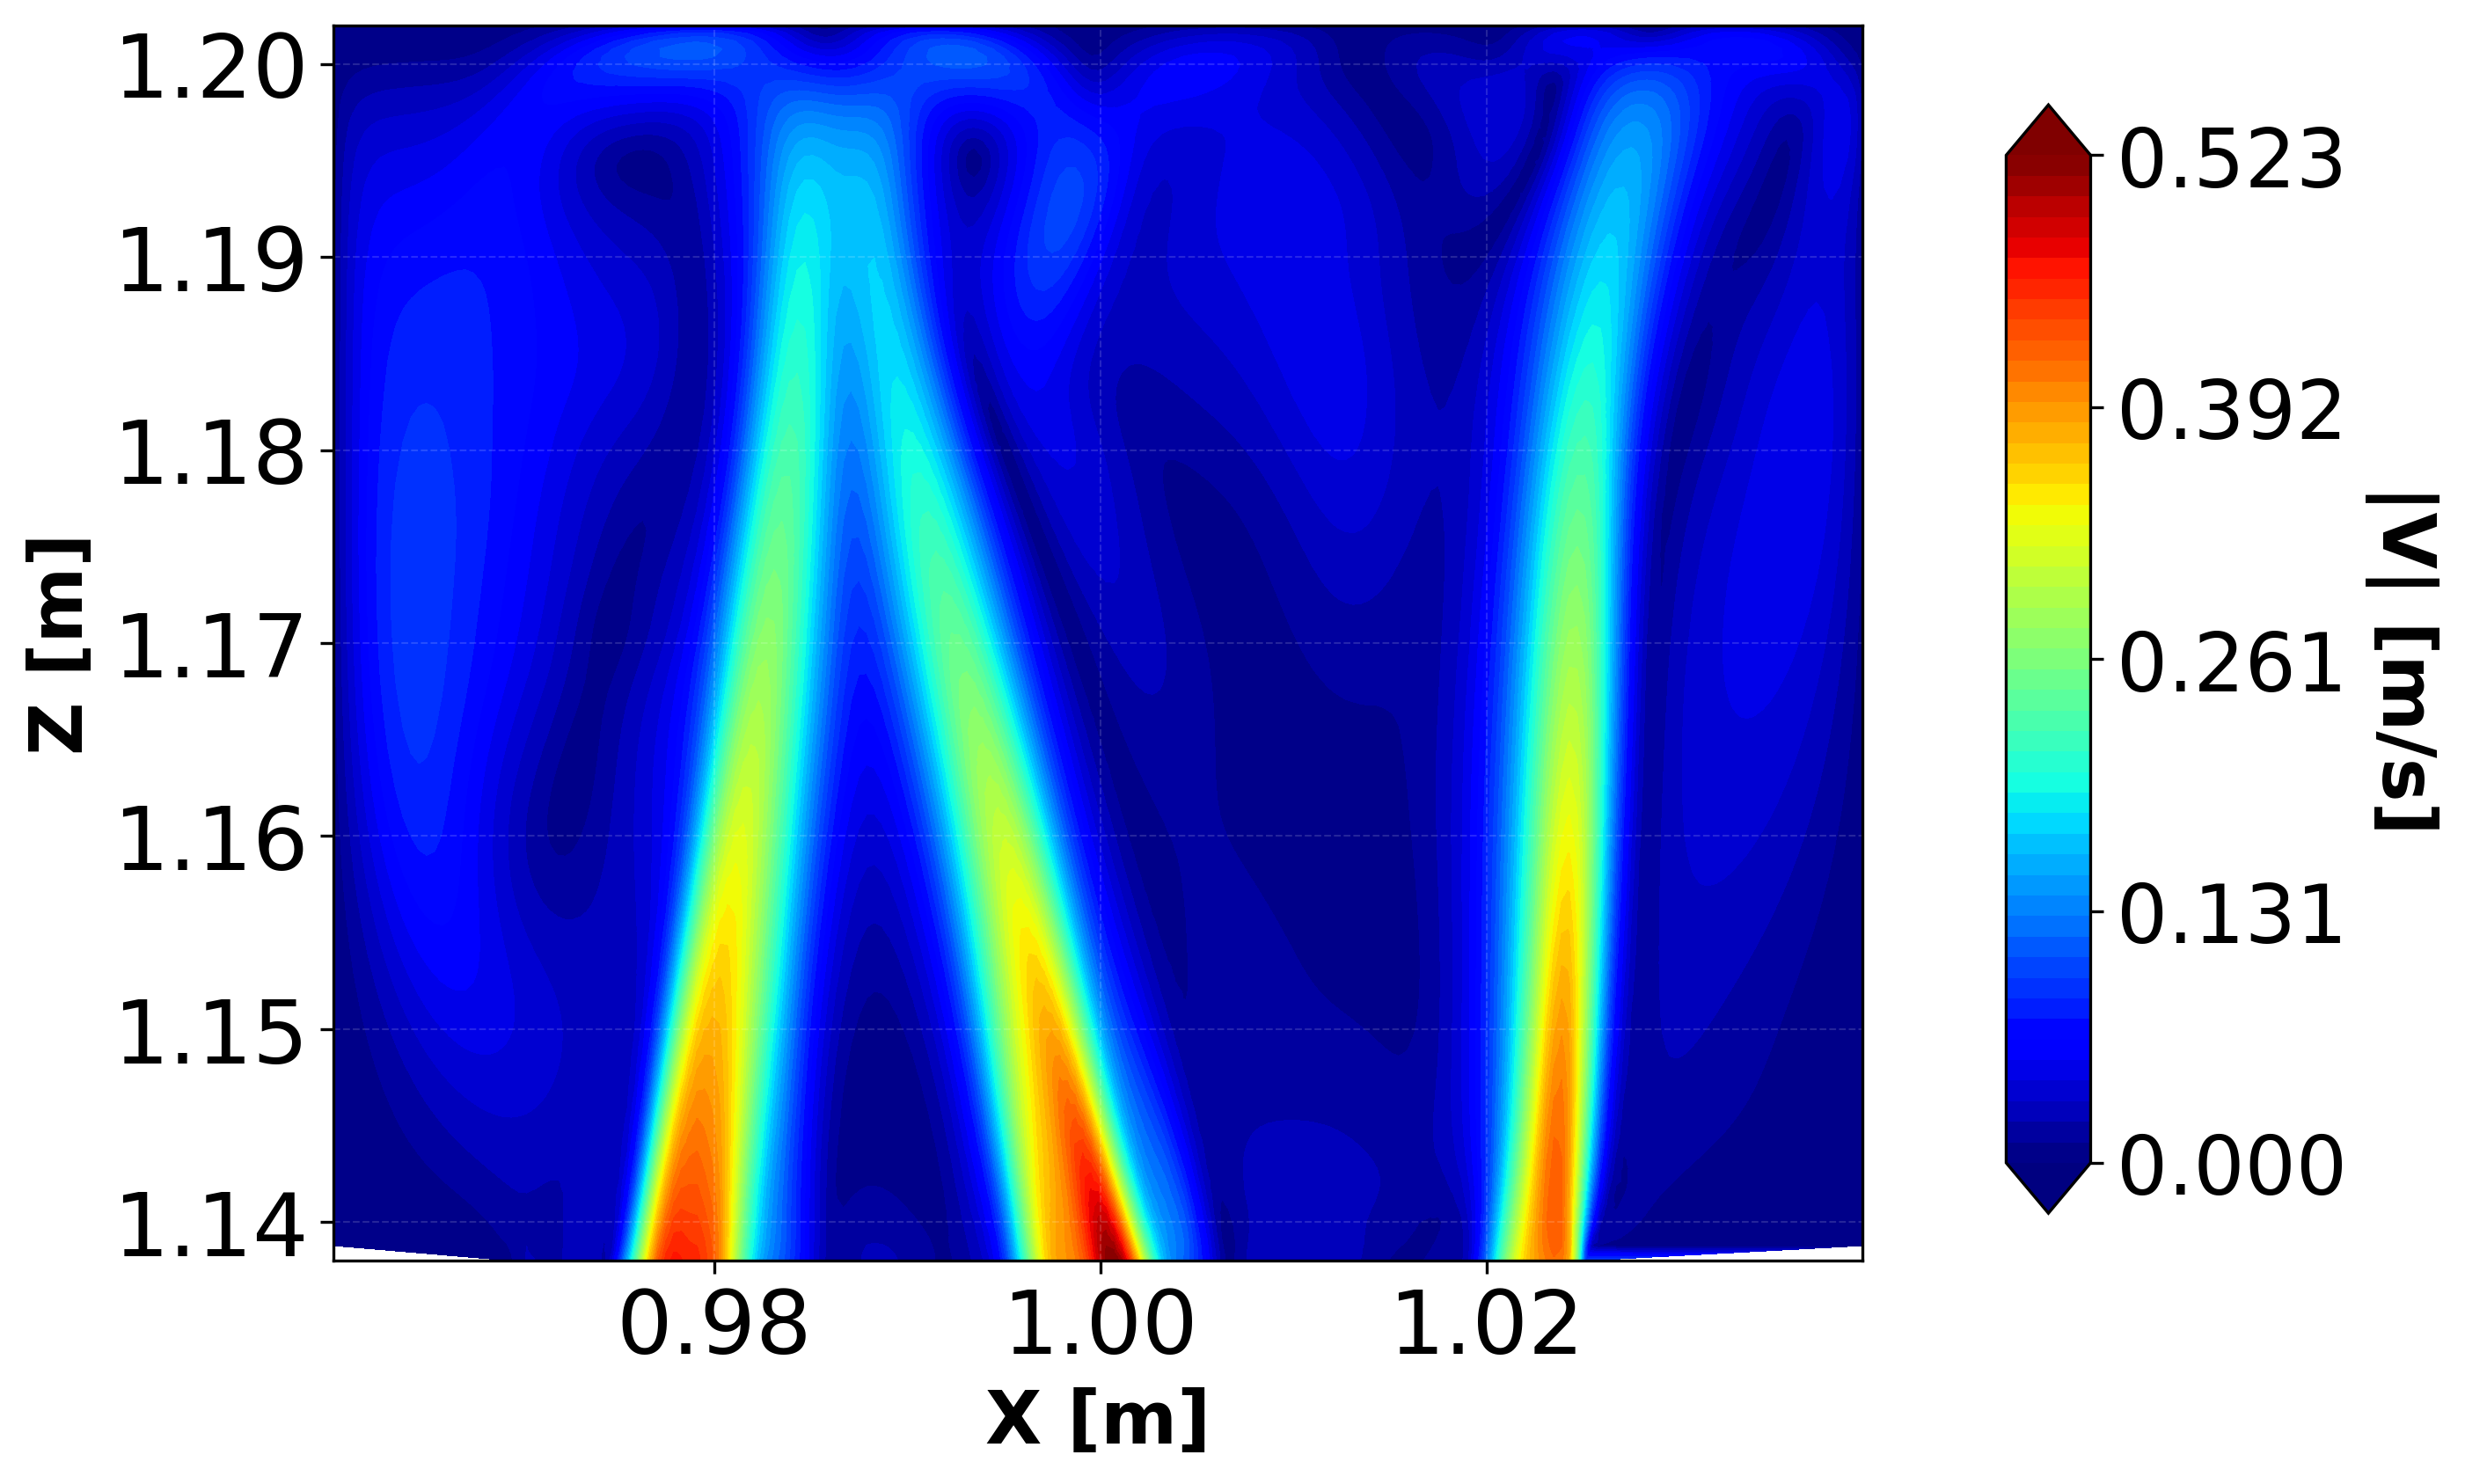
\includegraphics[width=\linewidth]{grid_coarse.png}
    \caption{Coarse Mesh}
\end{subfigure}

\vspace{0.3cm}

\begin{subfigure}[b]{0.47\textwidth}
    \centering
    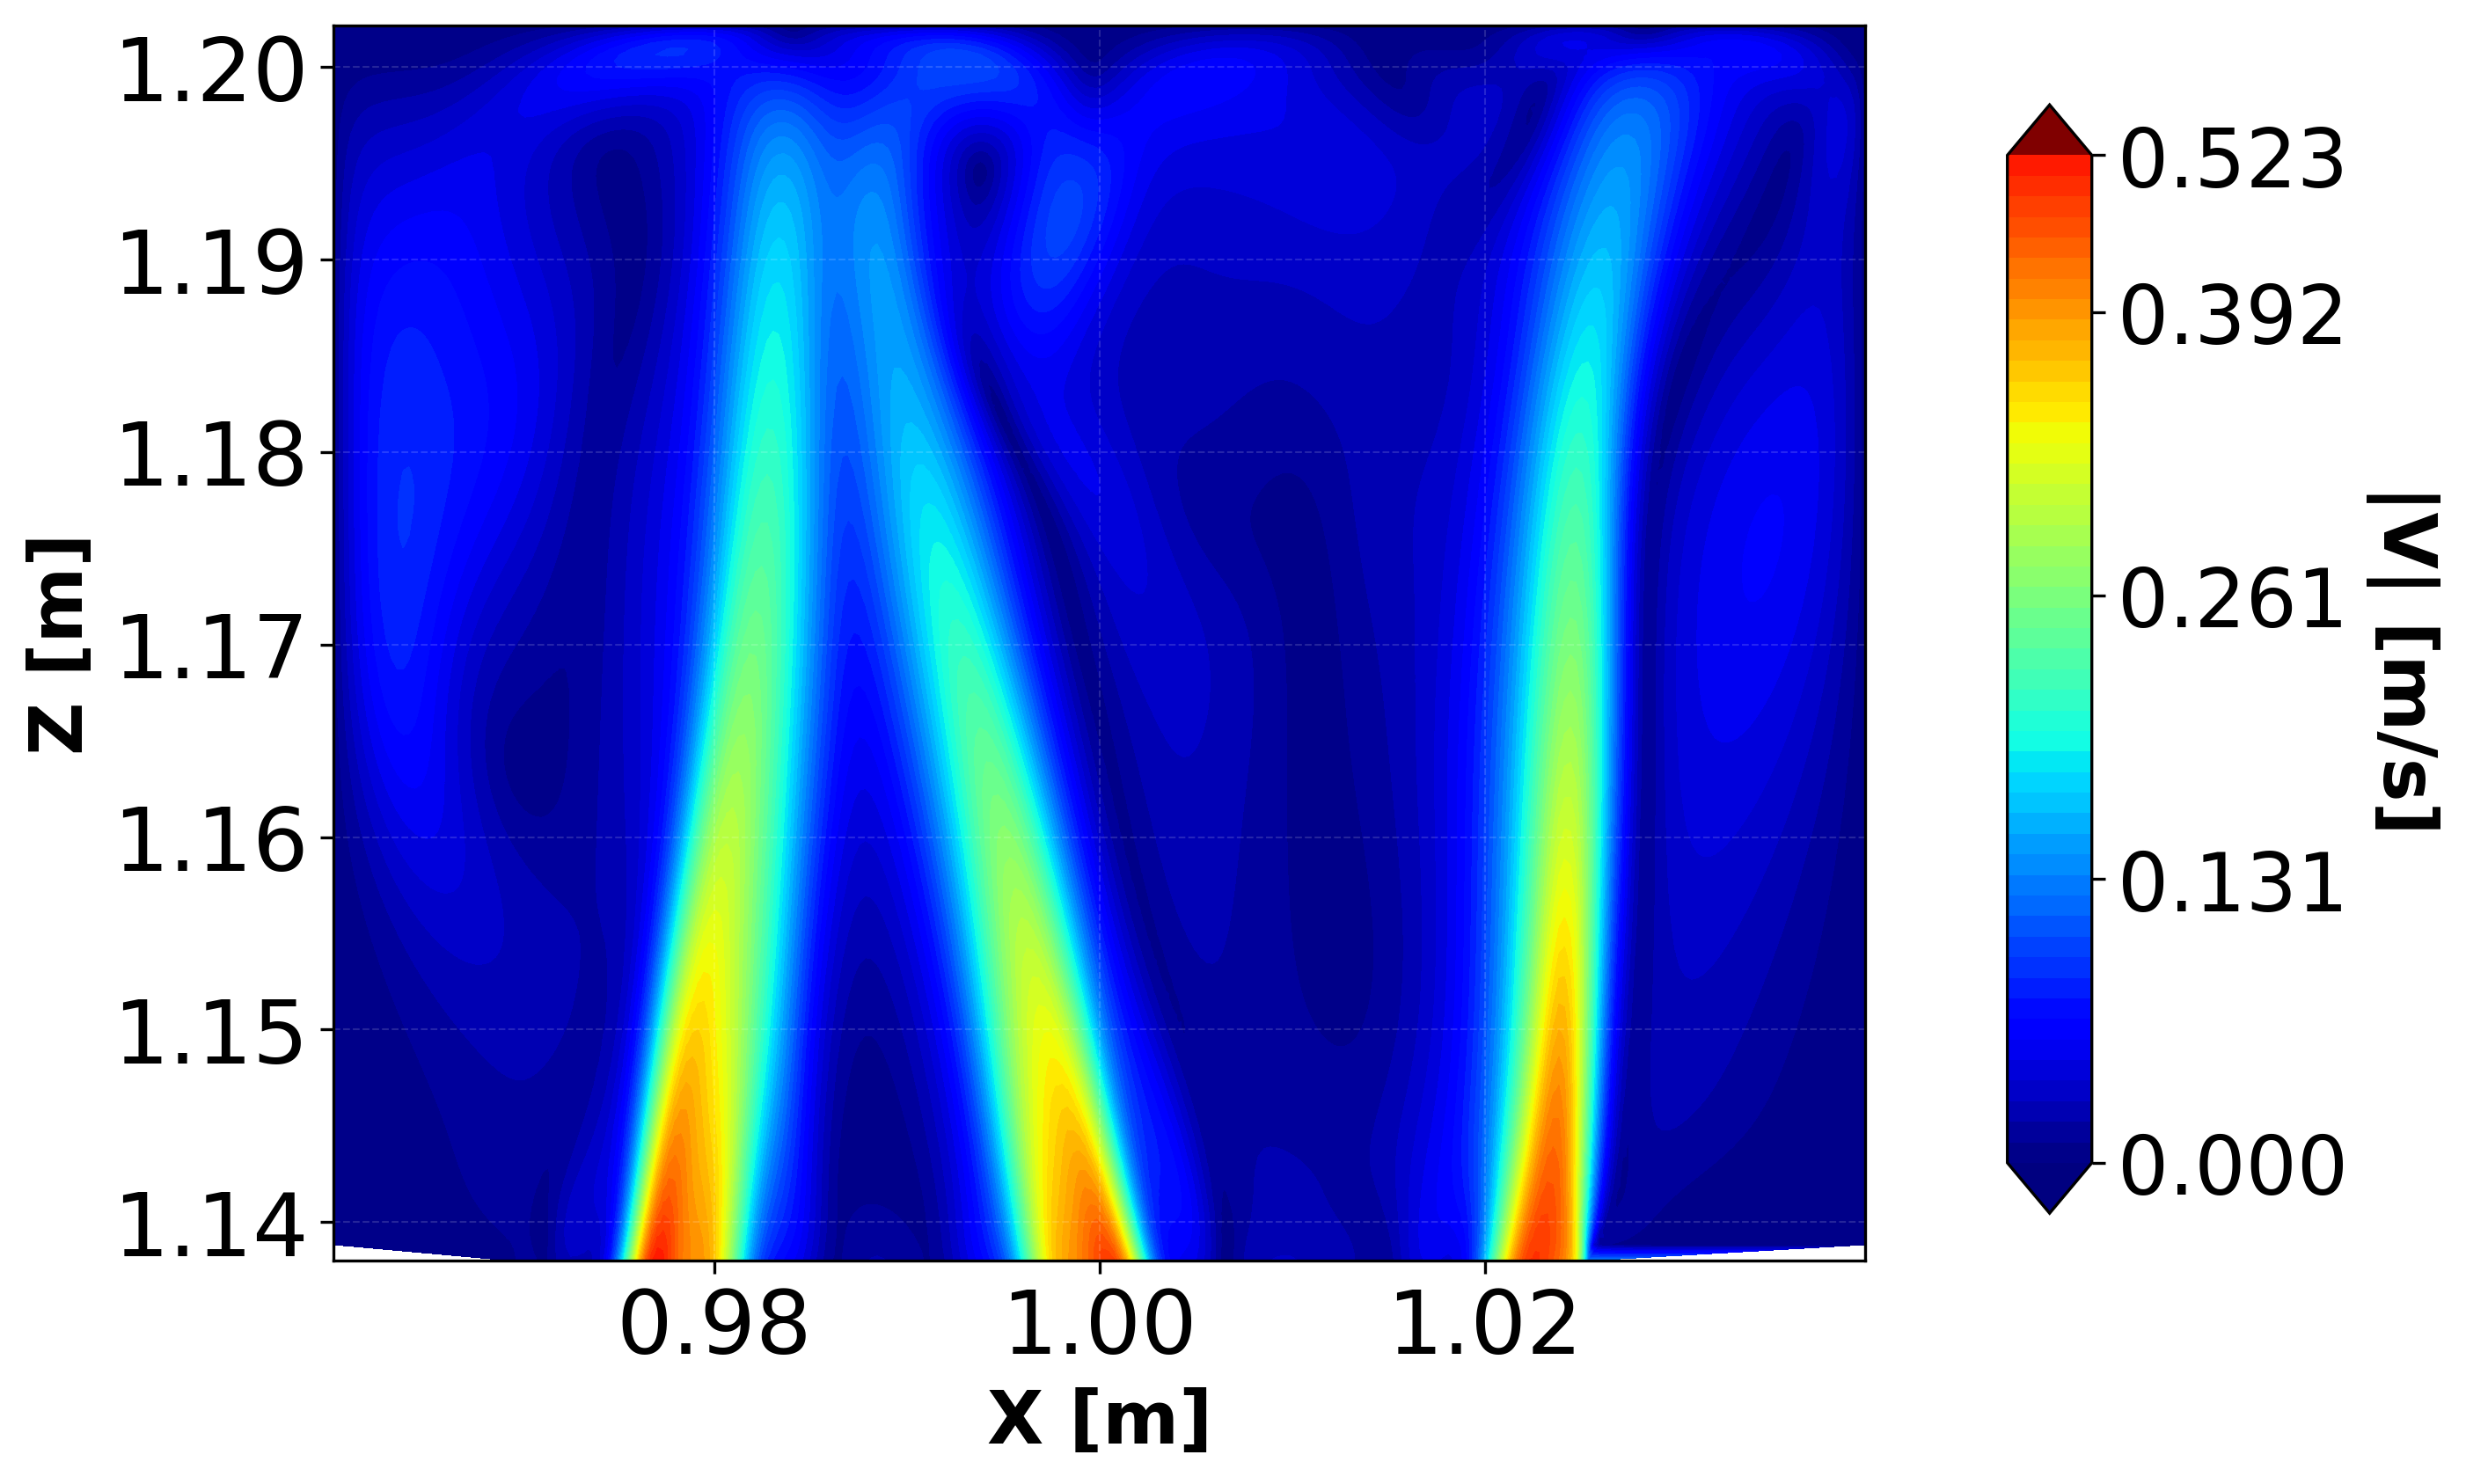
\includegraphics[width=\linewidth]{grid_medium.png}
    \caption{Medium Mesh}
\end{subfigure}
\hfill
\begin{subfigure}[b]{0.47\textwidth}
    \centering
    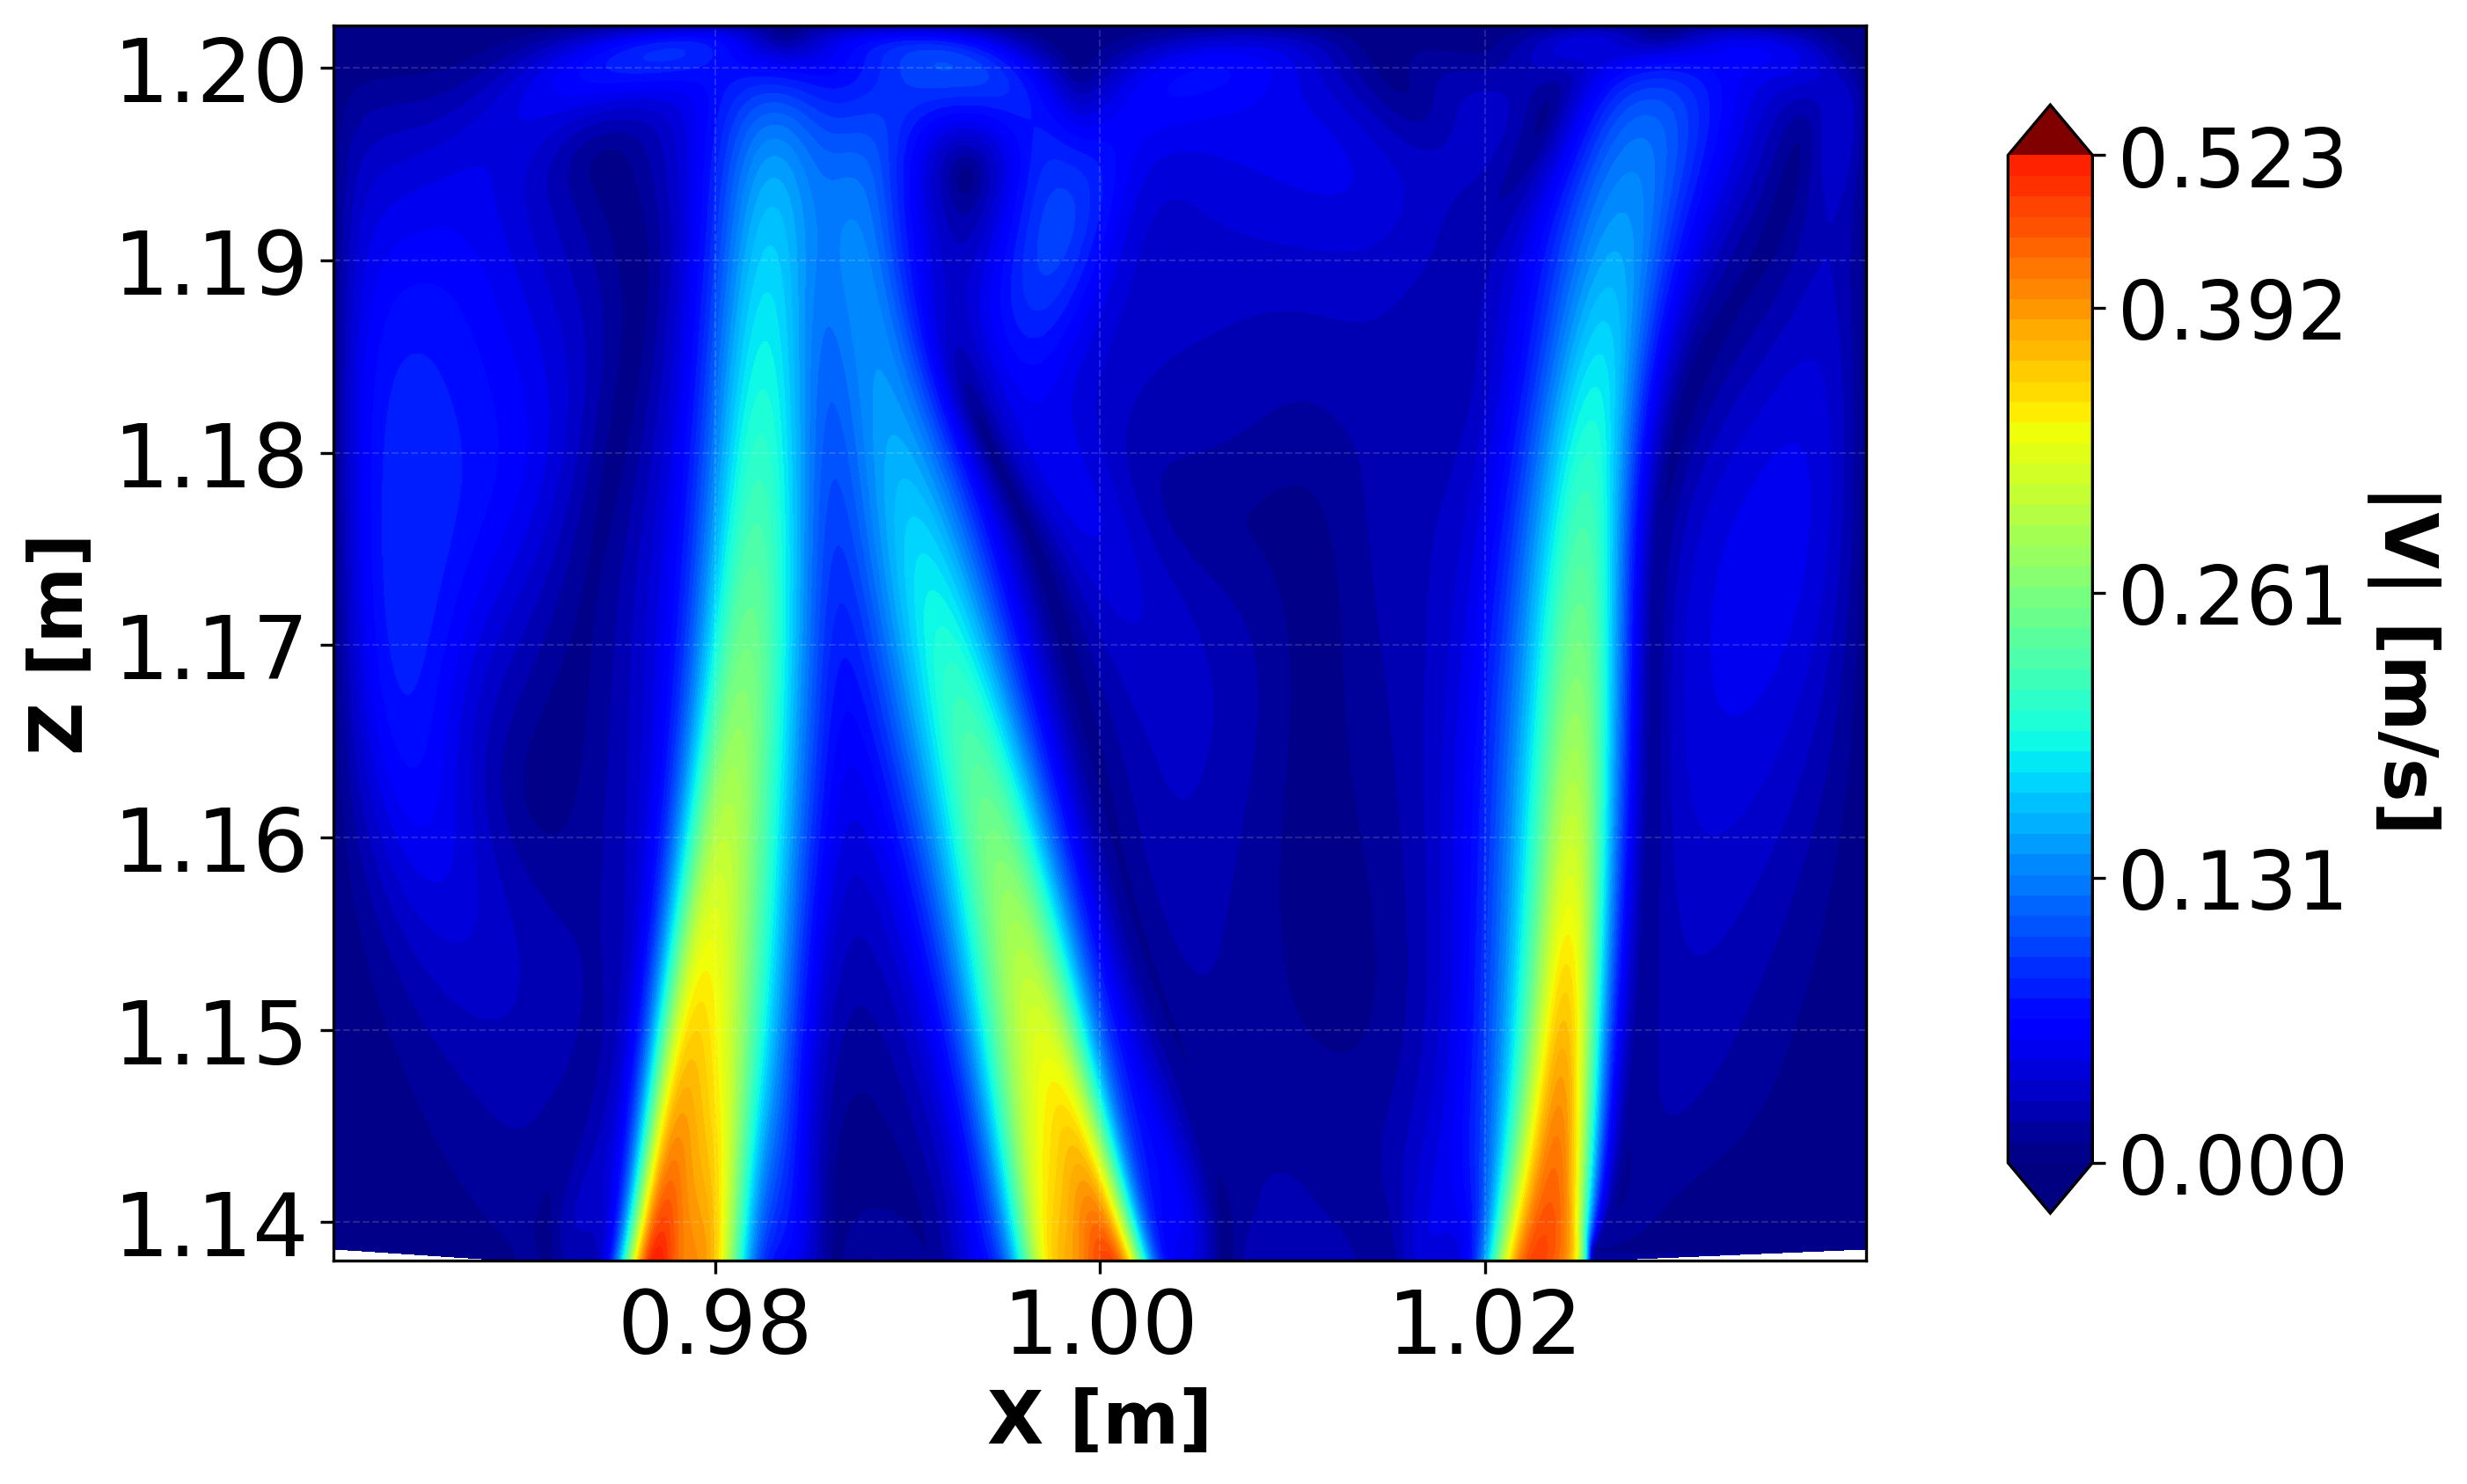
\includegraphics[width=\linewidth]{grid_fine.png}
    \caption{Fine Mesh}
\end{subfigure}
\caption{Grid sensitivity study on a representative subdomain of the regular packing with $\theta=40^\circ$. (a)~Geometry showing the extraction plane position for grid convergence assessment. (b-d)~Time-averaged fields of velocity magnitude $|V|$ on the extraction surface for the three grid levels of Table~\ref{tab:grid}, keeping the same colour scale. The jet structure is preserved across all resolutions; the medium and fine fields are nearly identical, see Table~\ref{tab:grid} for quantitative values.}
\label{fig:grid}
\end{figure}

\subsection{Symmetry Verification}
\label{sec:numerics:symmetry}
As discussed previously, each element of the packing system contains four slits, resulting in four measurement planes that could, in principle, be analysed independently. Owing to the geometric arrangement of the slits, the measurement locations form two point-symmetric pairs about the column axis: Pos1 with Pos7, and Pos3 with Pos5 (Sec.~\ref{sec:geometry:coords}). As an internal consistency check, the simulations should therefore reproduce identical flow structures within each symmetric pair for fully laminar conditions.
Fig.~\ref{fig:symmetry} compares the time-averaged velocity-magnitude contours and in-plane streamlines for both symmetric pairs, Pos3/Pos5 and Pos1/Pos7, for the packing with $\theta=30^\circ$ at Re$_p=100$. Within each pair the two planes \deleted{show close mirror symmetry}\added{map approximately onto each other under the point symmetry, which within the plane appears as a mirror reflection}: the central high-velocity jet, the neighbouring slit jets, and the recirculation regions map approximately onto their reflected counterparts. The accompanying profiles of velocity magnitude compared for the two gaps at four streamwise heights (Fig.~\ref{fig:symmetry}b,d) agree closely within each pair once the $x$ coordinate of the profiles at Pos5 and Pos7 is mirrored ($x\to-x$, consistent with the opposite signs of $a_{\mathrm{Pos},n}$ in Table~\ref{tab:pos}). The central jet and the positions of the side peaks agree, but the magnitudes of some side peaks differ. For example, at $z=180$\,mm the Pos3 side peak near $x\approx-0.03$\,m reaches about $0.43$\,m/s, whereas Pos5 shows only about $0.08$\,m/s at the same location. The symmetry is therefore approximate rather than exact. Each symmetric pair nevertheless carries largely equivalent flow information, so only one representative plane from each pair is retained for the detailed analysis presented in the following sections. This reduces the amount of analysed data, but the side-peak differences noted above are not represented by the retained planes.
\begin{figure}[tbp]
\centering
\captionsetup[subfigure]{skip=0pt}
\subfloat[Pos3 vs Pos5: velocity-magnitude contours with in-plane streamlines]{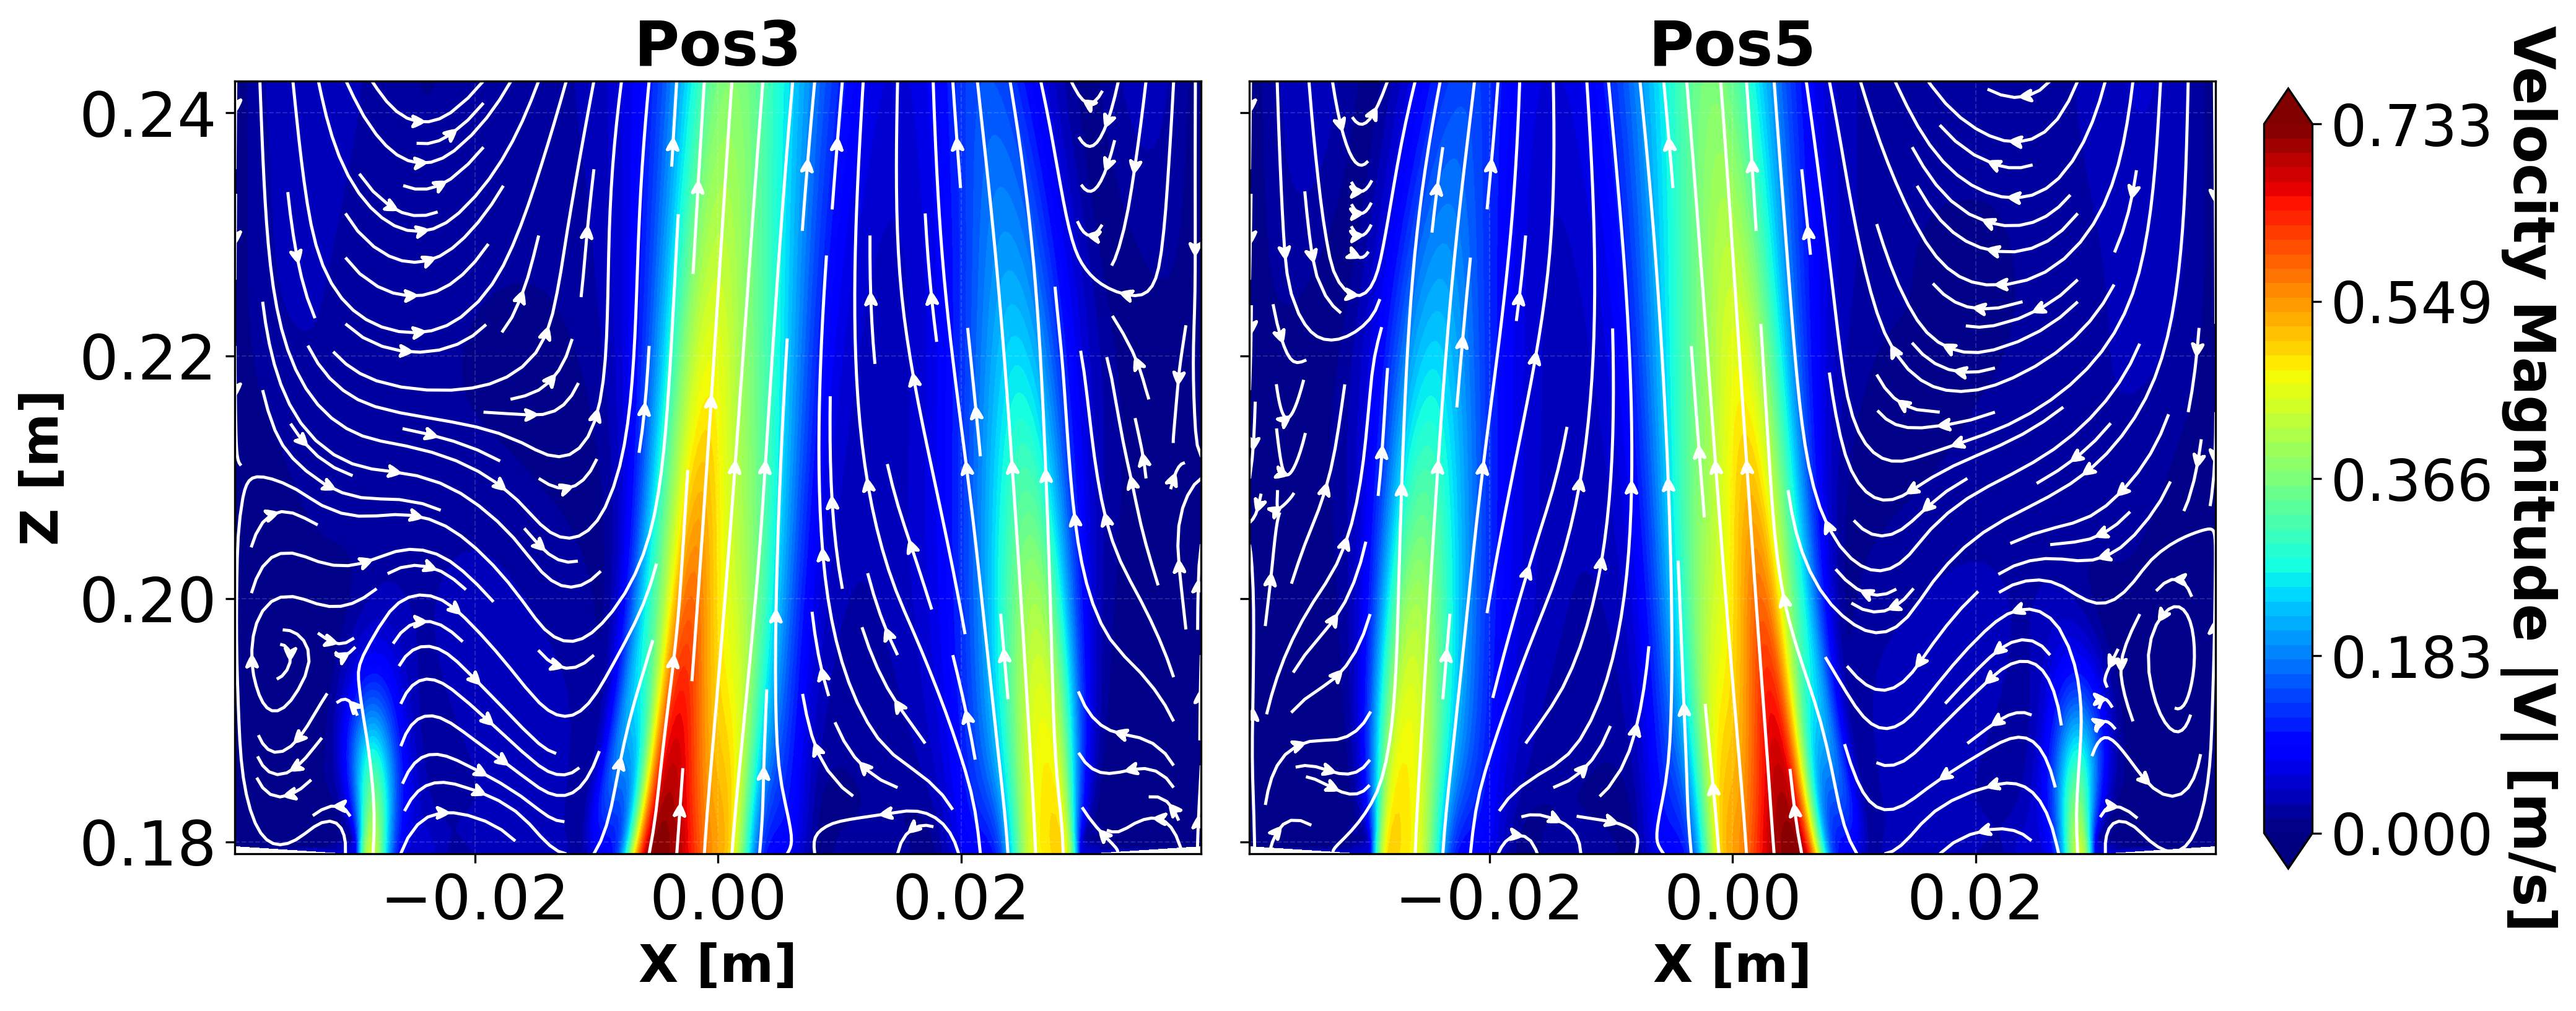
\includegraphics[width=0.7\linewidth]{symmetry/Symmetry_Contour_PosPos3.png}}\\
\subfloat[Pos3 vs Pos5: velocity-magnitude line profiles after mirroring $x$ for Pos5]{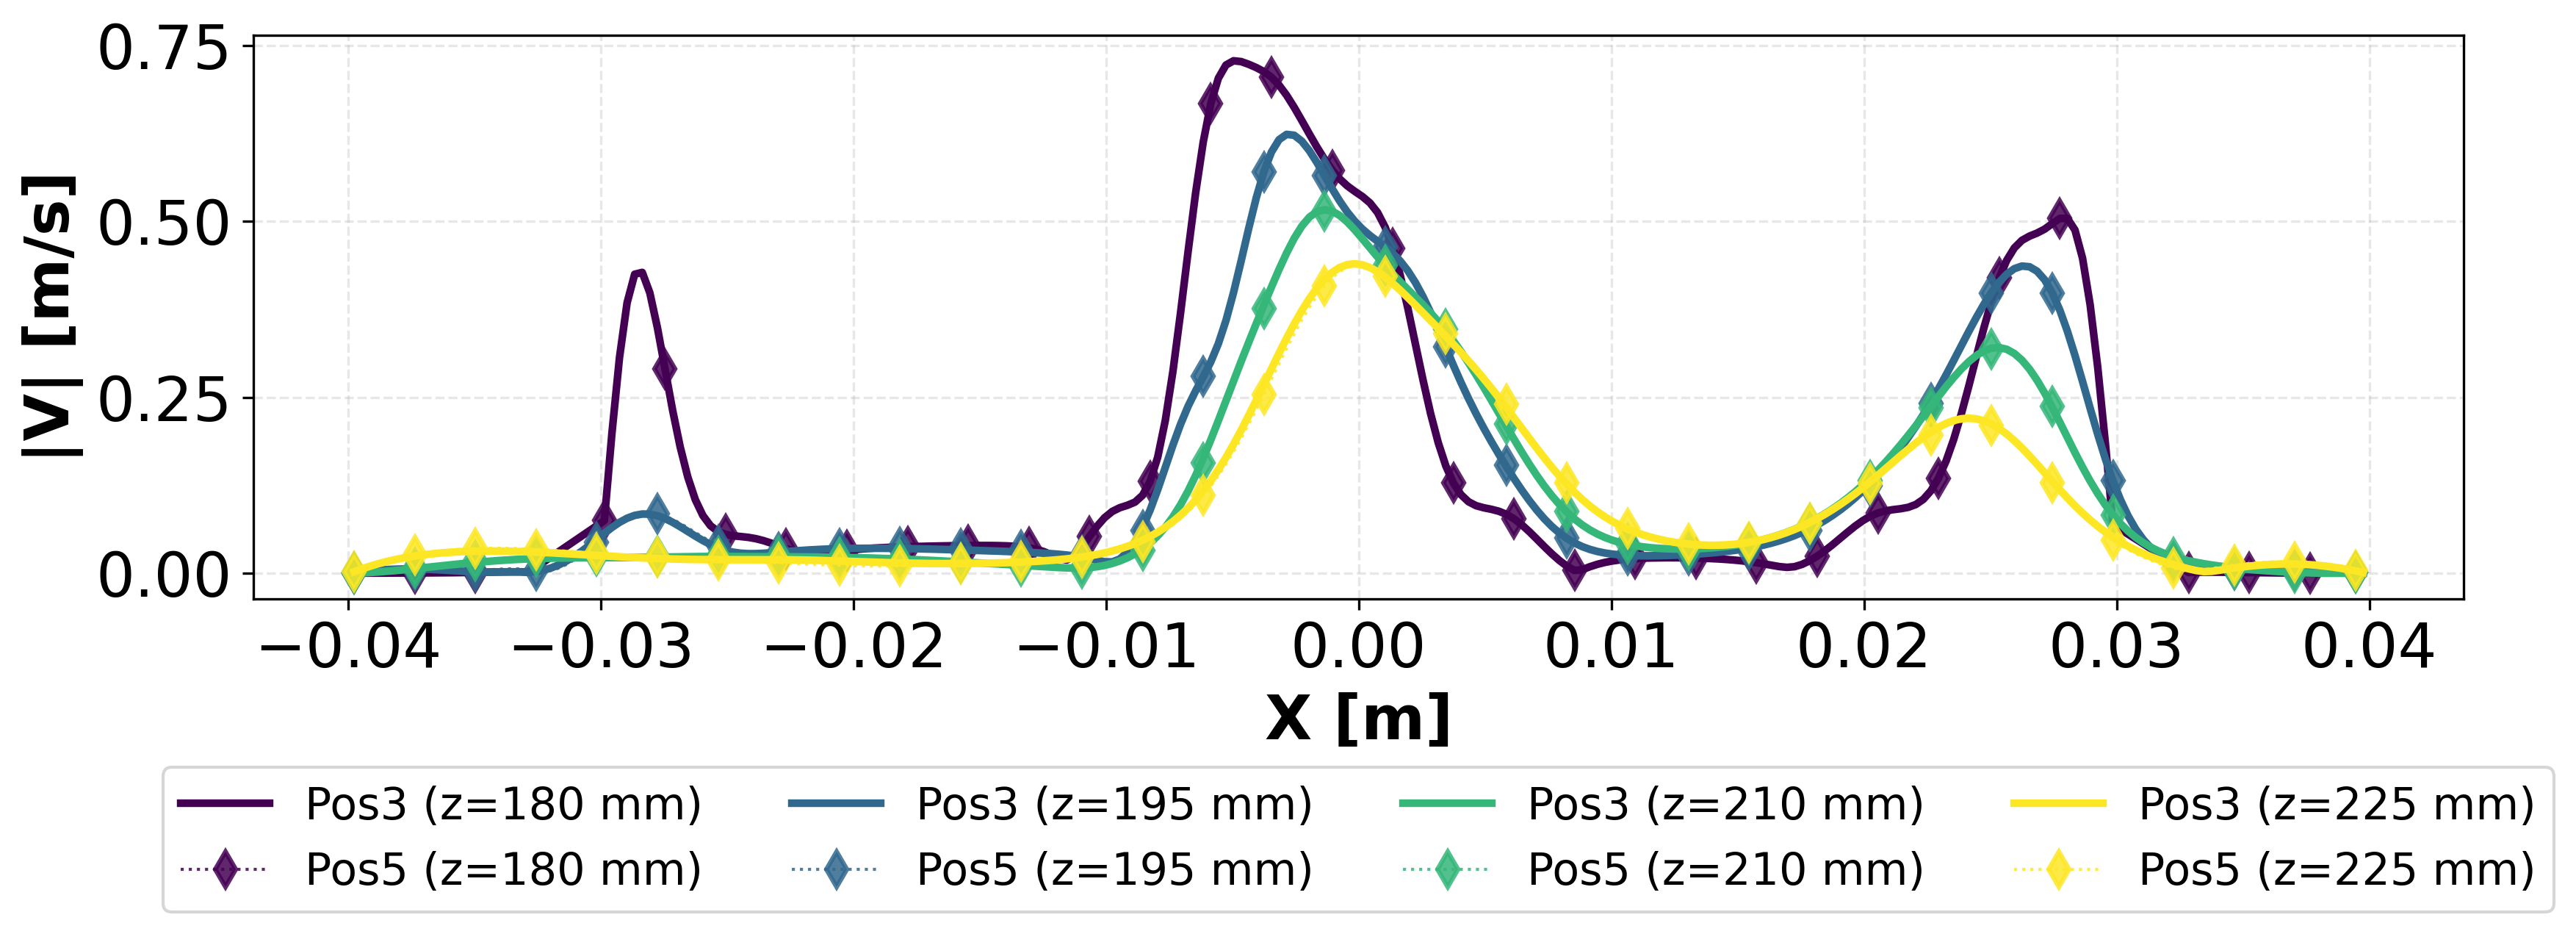
\includegraphics[width=0.7\linewidth]{symmetry/Combined_Line_Profiles_Pos3.png}}\\
\subfloat[Pos1 vs Pos7: velocity-magnitude contours with in-plane streamlines]{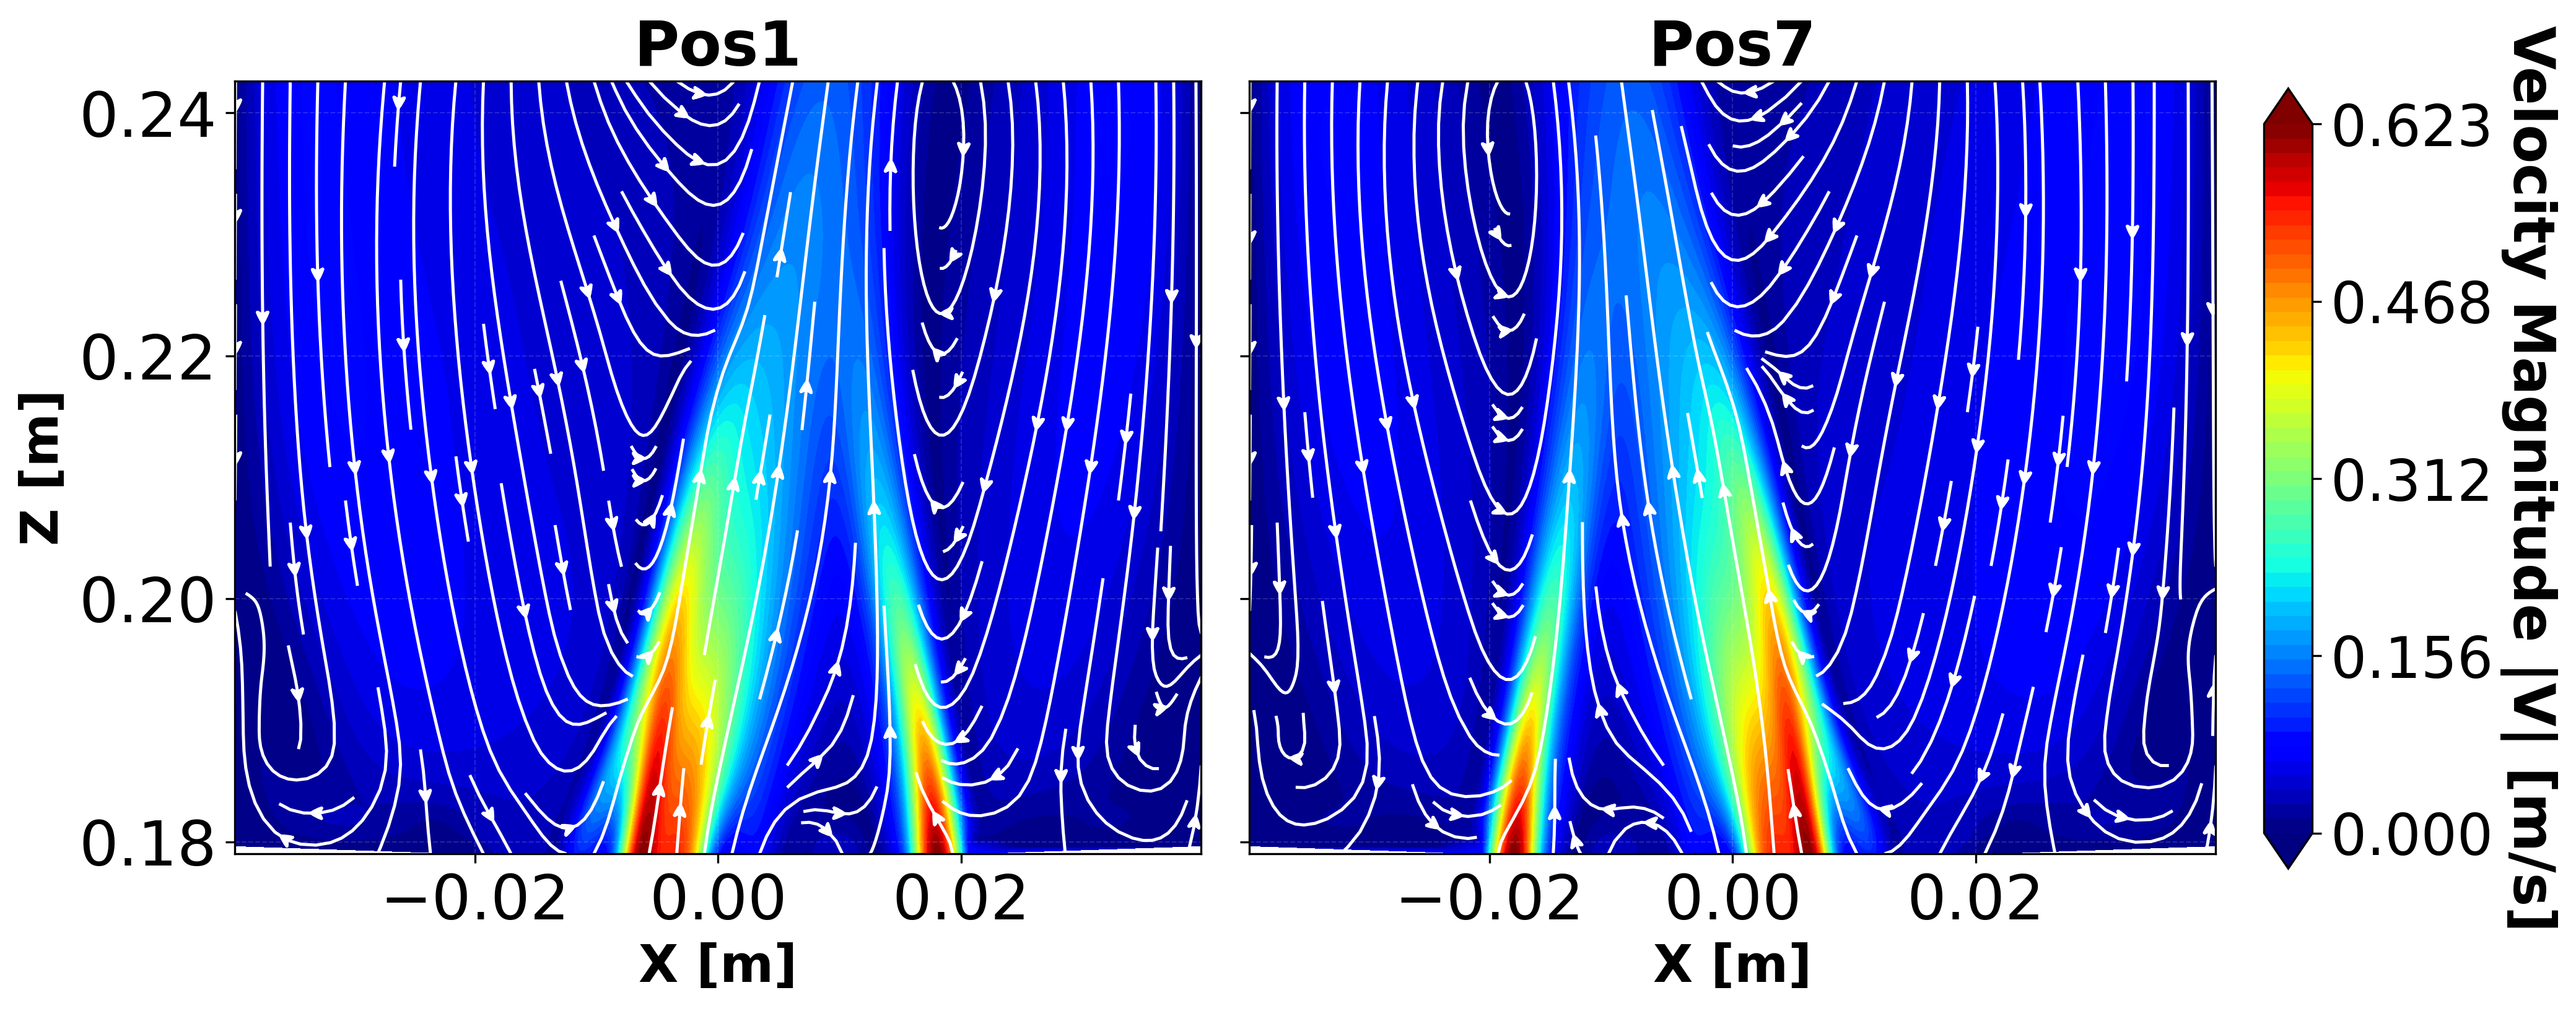
\includegraphics[width=0.7\linewidth]{symmetry/Symmetry_Contour_PosPos1.png}}
\caption{Symmetry verification for the $30^\circ$ packing at Re$_p = 100$, for the two point-symmetric measurement pairs. (a,b)~Pos3 and Pos5; (c,d)~Pos1 and Pos7. (a,c)~Time-averaged contours of velocity magnitude with in-plane streamlines, showing that each plane approximately maps onto the mirror image of its partner. 
(b,d)~Line profiles of time-averaged velocity magnitude across the gaps at four streamwise heights, 
comparing each plane (solid lines) with its point-symmetric partner (symbols) plotted after inverting the $x$ coordinate. 
The central jets of both pairs coincide closely, whereas the magnitudes of some side peaks differ (e.g., Pos3 vs Pos5 at $z=180$\,mm), so the symmetry of the simulated mean flow is approximate.}
\label{fig:symmetry}
\end{figure}
\clearpage
\begin{figure}[tbp]
\centering
\captionsetup[subfigure]{skip=0pt}
\setcounter{subfigure}{3}
\addtocounter{figure}{-1}
\subfloat[Pos1 vs Pos7: velocity-magnitude line profiles after mirroring $x$ for Pos7]{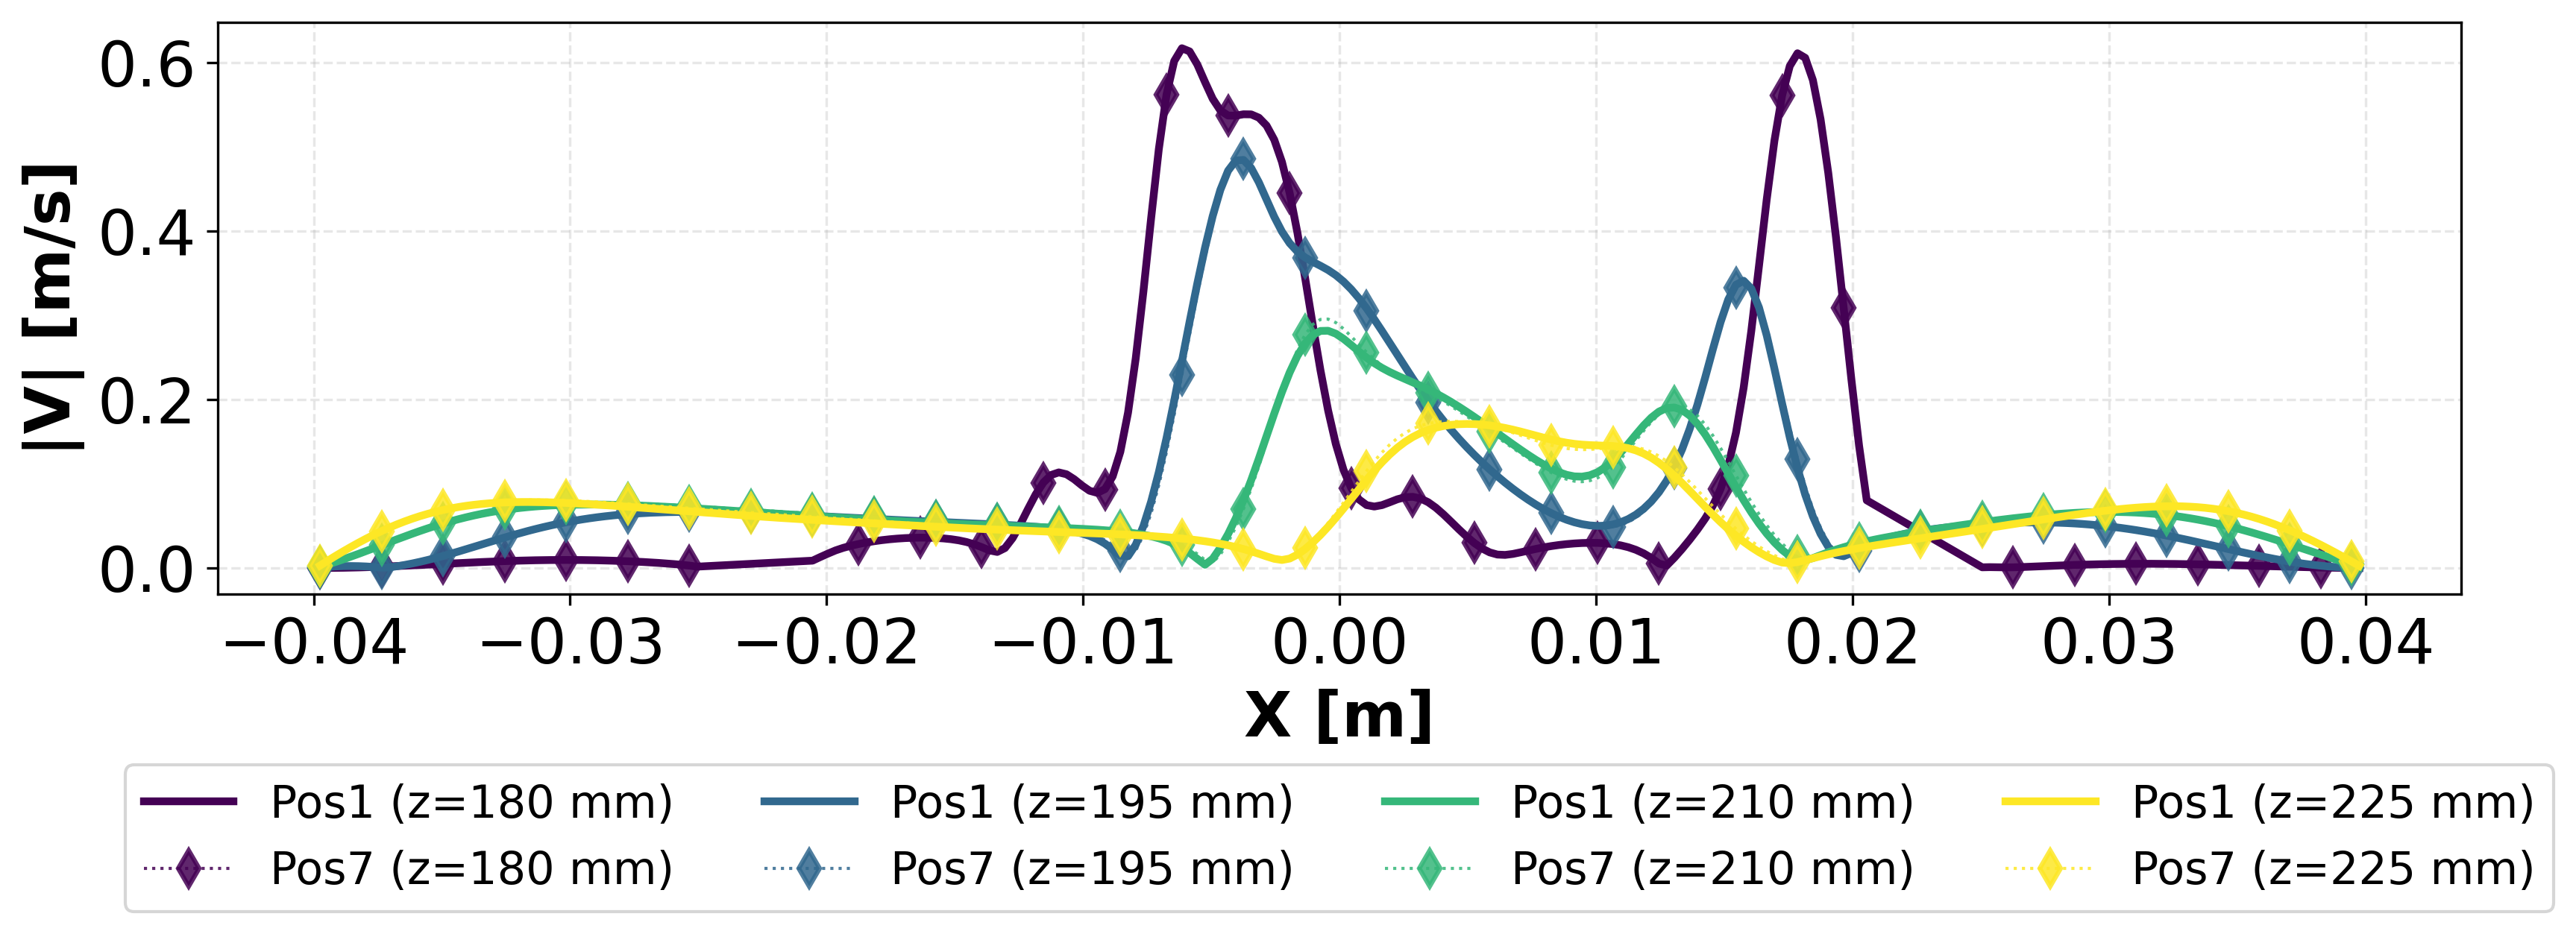
\includegraphics[width=0.7\linewidth]{symmetry/Combined_Line_Profiles_Pos1.png}}
\caption{Symmetry verification for the $30^\circ$ packing at Re$_p = 100$ (continued from the previous page).}
\end{figure}

\subsection{Validation against PIV Measurements}\label{sec:validation}
The accuracy of the numerical solver is then assessed by validating the predicted flow behaviour within the packing against experimental measurements.
The simulation results for the two periodic packing topologies are compared with the published PIV data of~\cite{velten2026,velten2026b}. The work on the irregular packing is still in progress, and its PIV data are not yet published. This validation section is organised into three stages. First, the comparison methodology and error metrics are introduced; second, the time-averaged fields of velocity magnitude on the measurement planes at the freeboard, just after leaving the packing, are assessed for validation; and finally, the layer-resolved development of the flow in the gaps within the packing is examined.

\subsubsection{Comparison Procedure and Error Metrics}
\label{sec:validation:procedure}

Velocity data are reported in the same in-plane coordinate system as used by~\cite{velten2026} consisting of the horizontal in-plane direction $x'$ and the vertical streamwise direction $z$. Simulation planes are extracted at the physical positions corresponding to Pos1 and Pos3 ($a_{\mathrm{Pos},1} = -22.5$ and $a_{\mathrm{Pos},3} = -7.5\,\mathrm{mm}$ from the reactor centre, Table~\ref{tab:pos}). Each plane extracted from the simulations is masked to show only the fluid region, interpolated onto the experimental PIV measurement grid (vector resolution $3.40$-$3.44\,\mathrm{vec/mm}$, Table~2 of \cite{velten2026}), and finally compared with the measured field point by point.

Agreement is quantified on the time-averaged velocity magnitude $|V|$ over all $M$ fluid grid points of a plane. Denoting the simulated and experimental values of velocity magnitude at point $i$ by $s_i$ and $e_i$, respectively, we report the root-mean-square error
\begin{equation}
    \mathrm{RMSE} = \sqrt{\frac{1}{M}\sum_{i=1}^{M}\left(s_i-e_i\right)^2},
\end{equation}
normalised by the experimental dynamic range ($\mathrm{NRMSE}$),
\begin{equation}
\mathrm{NRMSE} = \frac{\mathrm{RMSE}}{e_\mathrm{max}-e_\mathrm{min}},
    \label{eq:rmse}
\end{equation}
the coefficient of determination $R^2 = 1-\sum_i(s_i-e_i)^2/\sum_i(e_i-\bar{e})^2$ measures how much of the spatial variance of the measured field is reproduced. $\mathrm{NRMSE}$ is the primary headline metric, as it is insensitive to the absolute velocity level and is therefore comparable across all topologies and Reynolds numbers.

\subsubsection{Velocity Fields at the Freeboard}
\label{sec:validation:surface}

The simulation results are first validated using the time-averaged velocity fields at the freeboard, just above the packing after leaving element L18. There, large-scale flow features can be directly compared. The aim is to establish that the numerical model reproduces both the spatial organisation of the flow and the corresponding absolute velocity levels over the entire measurement plane.

Figs.~\ref{fig:validation_surface_re100} and~\ref{fig:validation_surface_re300} compare the simulated and measured fields of velocity magnitude, with superposed in-plane streamlines, for the regular packing with $\theta=30^\circ$ at Pos3 and Re$_p=100$ (Fig.~\ref{fig:validation_surface_re100}) or Re$_p=300$ (Fig.~\ref{fig:validation_surface_re300}). At both Reynolds numbers the flow organises into discrete streamwise jets issuing from the outlet slits and separated by low-velocity wakes, with a strong central jet flanked by weaker side jets. The simulation accurately reproduces the number, location, width, and peak magnitude of these jets, as well as the streamline topology of the intervening recirculation zones. Notably, the agreement remains strong for both Re$_p=100$ and Re$_p=300$, showing that the model retains its predictive capability as the flow intensity increases. This agreement is further quantified by the line profiles in panel~(b) of each figure, which overlay the simulated and measured profiles of velocity magnitude at four streamwise heights for Pos3. The blue band marks $\pm1\sigma$ of the velocity fluctuations in the PIV data, i.e., the standard deviation $\sigma$ of the instantaneous fields about the time average, propagated to the velocity magnitude as $\sigma_{|V|}=\sqrt{(v_{x'}\sigma_{v_{x'}})^2+(v_z\sigma_{v_z})^2}/|V|$. It thus reflects mostly the flow unsteadiness, becoming more intense when increasing Re$_p$, as discussed in~\cite{velten2026b}. Despite minor deviations from the experimental data, the simulated profiles demonstrate good agreement with the measurements and reproduce all main flow features (jet peaks and positions, inter-jet minima), while remaining within or very close to the experimental range when taking into account fluctuations in time (blue band).

This level of agreement is preserved for both regular packings and Reynolds numbers. For $\theta=30^\circ$, the analysis delivers $\mathrm{NRMSE}=6\%$ and $R^2=0.92$ for Re$_p=100$, $\mathrm{NRMSE}=5\%$ and $R^2=0.95$ for Re$_p=300$. Note that the remaining discrepancies between simulations and measurements are not distributed uniformly. A detailed comparison shows that they are found mainly in the thin, high-gradient shear layers bordering the jets. This is also the location where the fluctuations are observed to be the highest in PIV. The largest visible differences are found for Re$_p=100$ at increasing distance after leaving the packing (in particular at $z=213$ mm, bottom right subfigure in Fig.~\ref{fig:validation_surface_re100}). This corresponds to the conditions where any perturbations coming from the surroundings of the experimental setup near the outlet would most strongly impact the features of this low-speed flow. It would also explain why the agreement is even better at Re$_p=300$.

Some of the remaining differences may also come from the numerical method itself. The solver ALBORZ is second-order accurate in space, which is consistent with the observed convergence order $p\approx2.1$ found in the grid study. \deleted{A scheme of this order acts like a small amount of extra viscosity. It hardly matters where the flow is smooth, but it smooths out features that vary over only a few grid cells, such as the thin shear layers next to the jets and the narrow jet peaks. A peak is then slightly lowered, and some of its momentum spreads into the slower fluid around it. This may be why some simulated peaks in the line profiles are a little lower and wider than the measured ones. The grid study shows that this effect is small at Re$_p=100$, where the peak velocity changes by only $0.5\%$ between the medium and fine grids. It matters more at Re$_p=300$, where the shear layers are thinner. Finer grids or a higher-order scheme, if needed, would be expected to bring the simulated peaks closer to the PIV results.}\added{The grid study shows, however, that the effect of the discretisation error on the jet peaks is small: at Re$_p=100$, the peak velocity changes by only $0.5\%$ between the medium and fine grids, and the coarse grid even yields a higher, not a lower, peak (Table~\ref{tab:grid}). At Re$_p=300$, the grid spacing was halved, whereas the shear-layer thickness decreases only by a factor of about $1/\sqrt{3}$; the shear layers are thus relatively better resolved there, in line with the better agreement at the freeboard. Discretisation errors are therefore unlikely to be the main origin of the remaining differences in peak velocities.}\remark{14}{The previous argument (numerical dissipation lowering the peaks, more so at Re$_p=300$) is contradicted by our own grid study and by the finer grid used at Re$_p=300$. The corresponding sentences in Sec.~\ref{sec:validation:layers} and in the Conclusions were adapted as well.}

\begin{figure}[tbp]
\centering
\subfloat[Time-averaged fields of velocity magnitude: Left, PIV; Right, simulation]{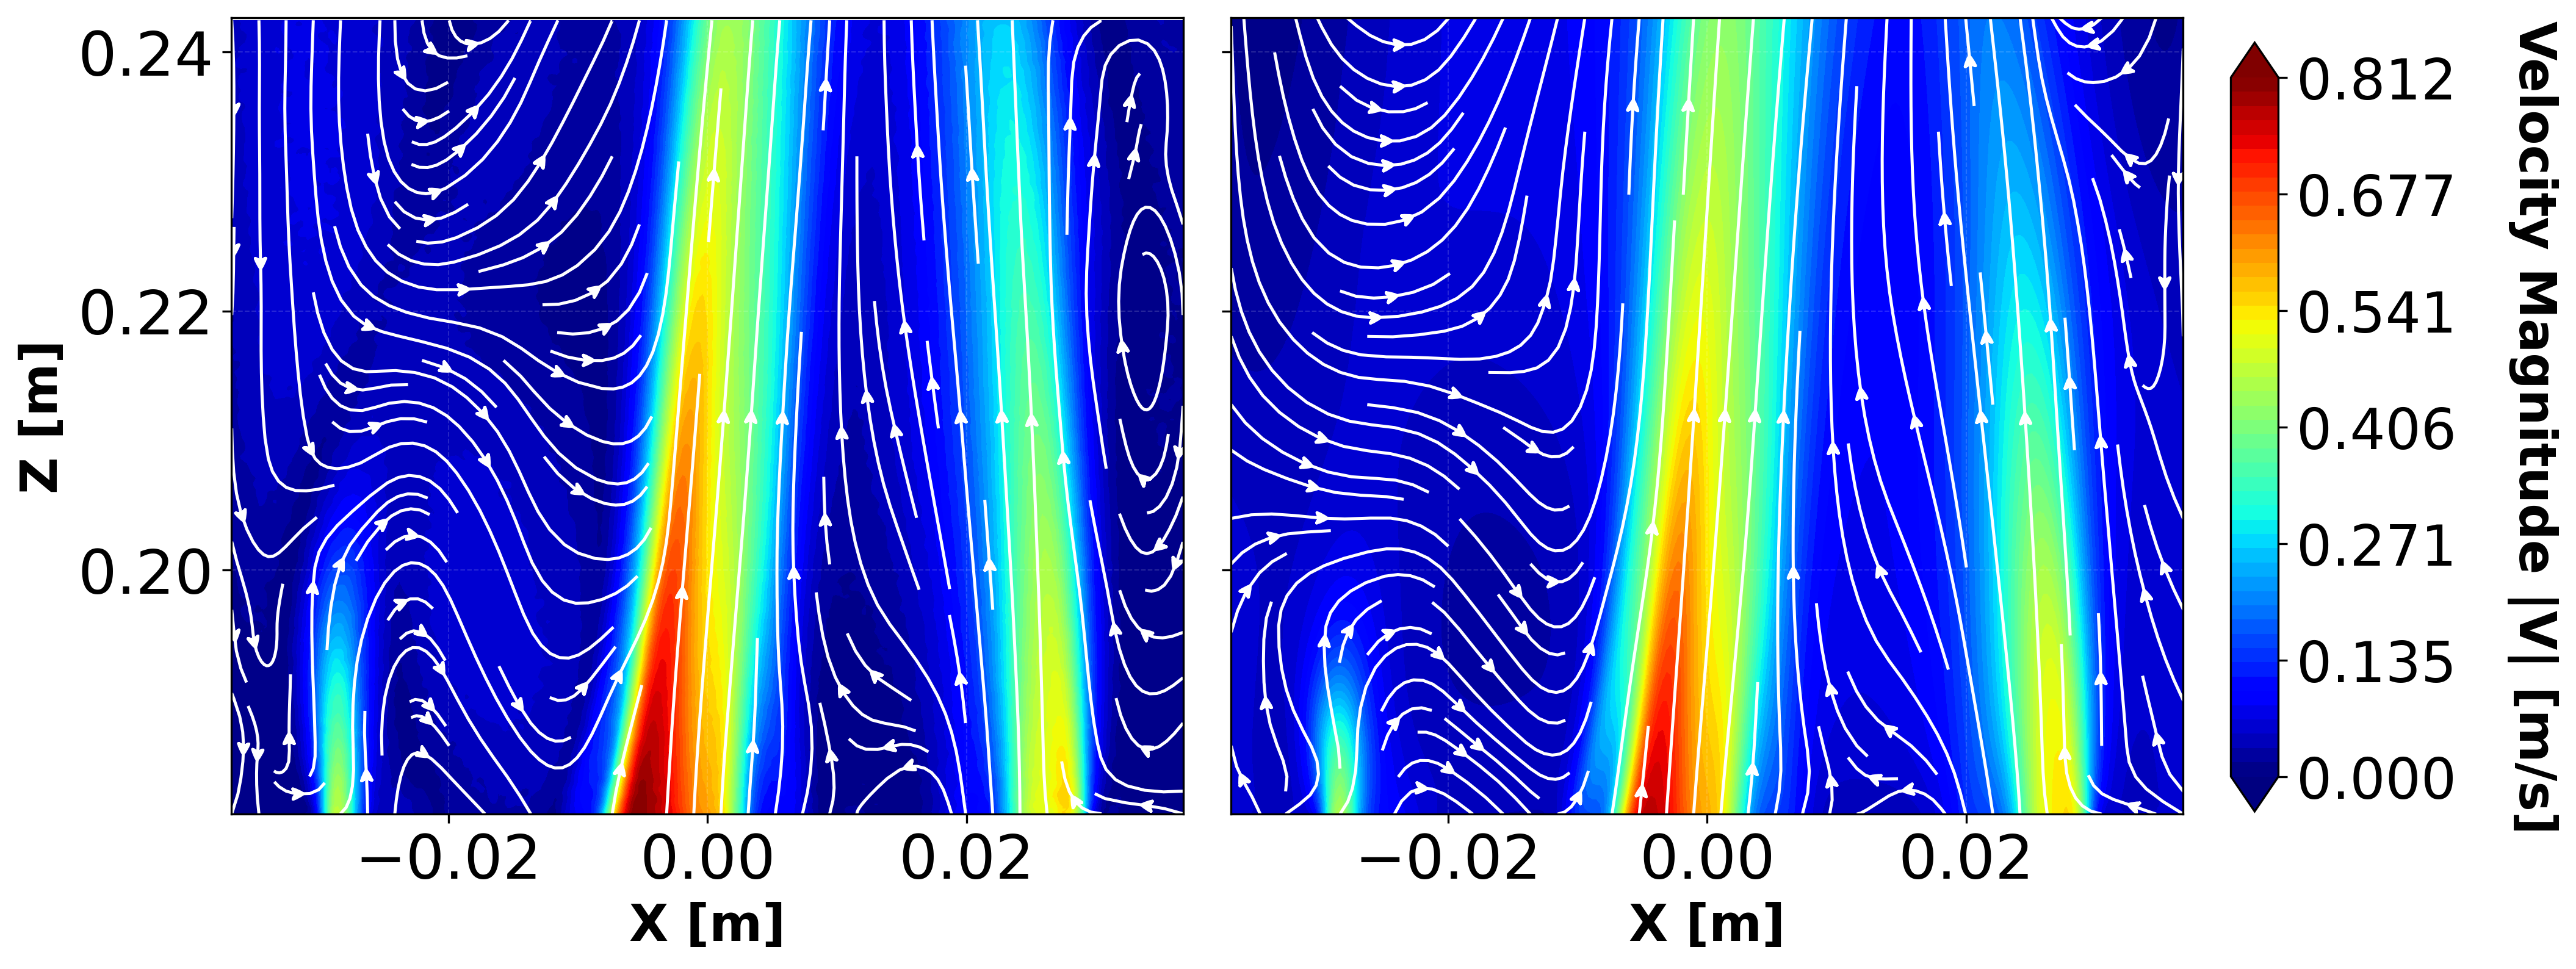
\includegraphics[width=0.95\linewidth]{30_Re_100/surface/pos3_Surface_plot.png}}\\
\subfloat[Profiles of velocity magnitude along horizontal lines]{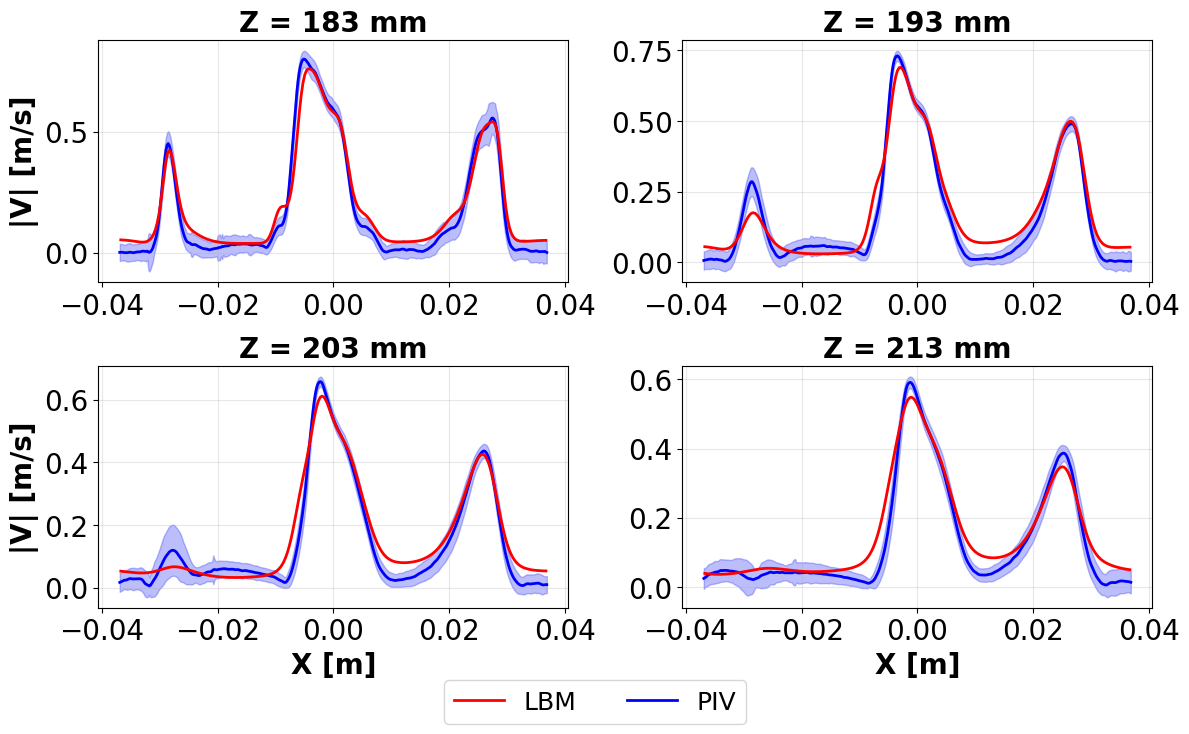
\includegraphics[width=0.95\linewidth]{30_Re_100/surface/Summary_Line_Profiles_Pos3.png}}
\caption{Validation at the freeboard for the packing with $\theta=30^\circ$ at Pos3 for Re$_p=100$: (a)~time-averaged fields of velocity magnitude with in-plane streamlines, experiment (left) vs. simulation (right); (b)~profiles of velocity magnitude across the plane at four streamwise heights, simulation (red) vs. PIV (blue) with the blue band showing $\pm1\sigma$ of the shot-to-shot velocity fluctuations in the PIV data.}
\label{fig:validation_surface_re100}
\end{figure}

\begin{figure}[tbp]
\centering
\subfloat[Time-averaged fields of velocity magnitude: Left, PIV; Right, simulation]{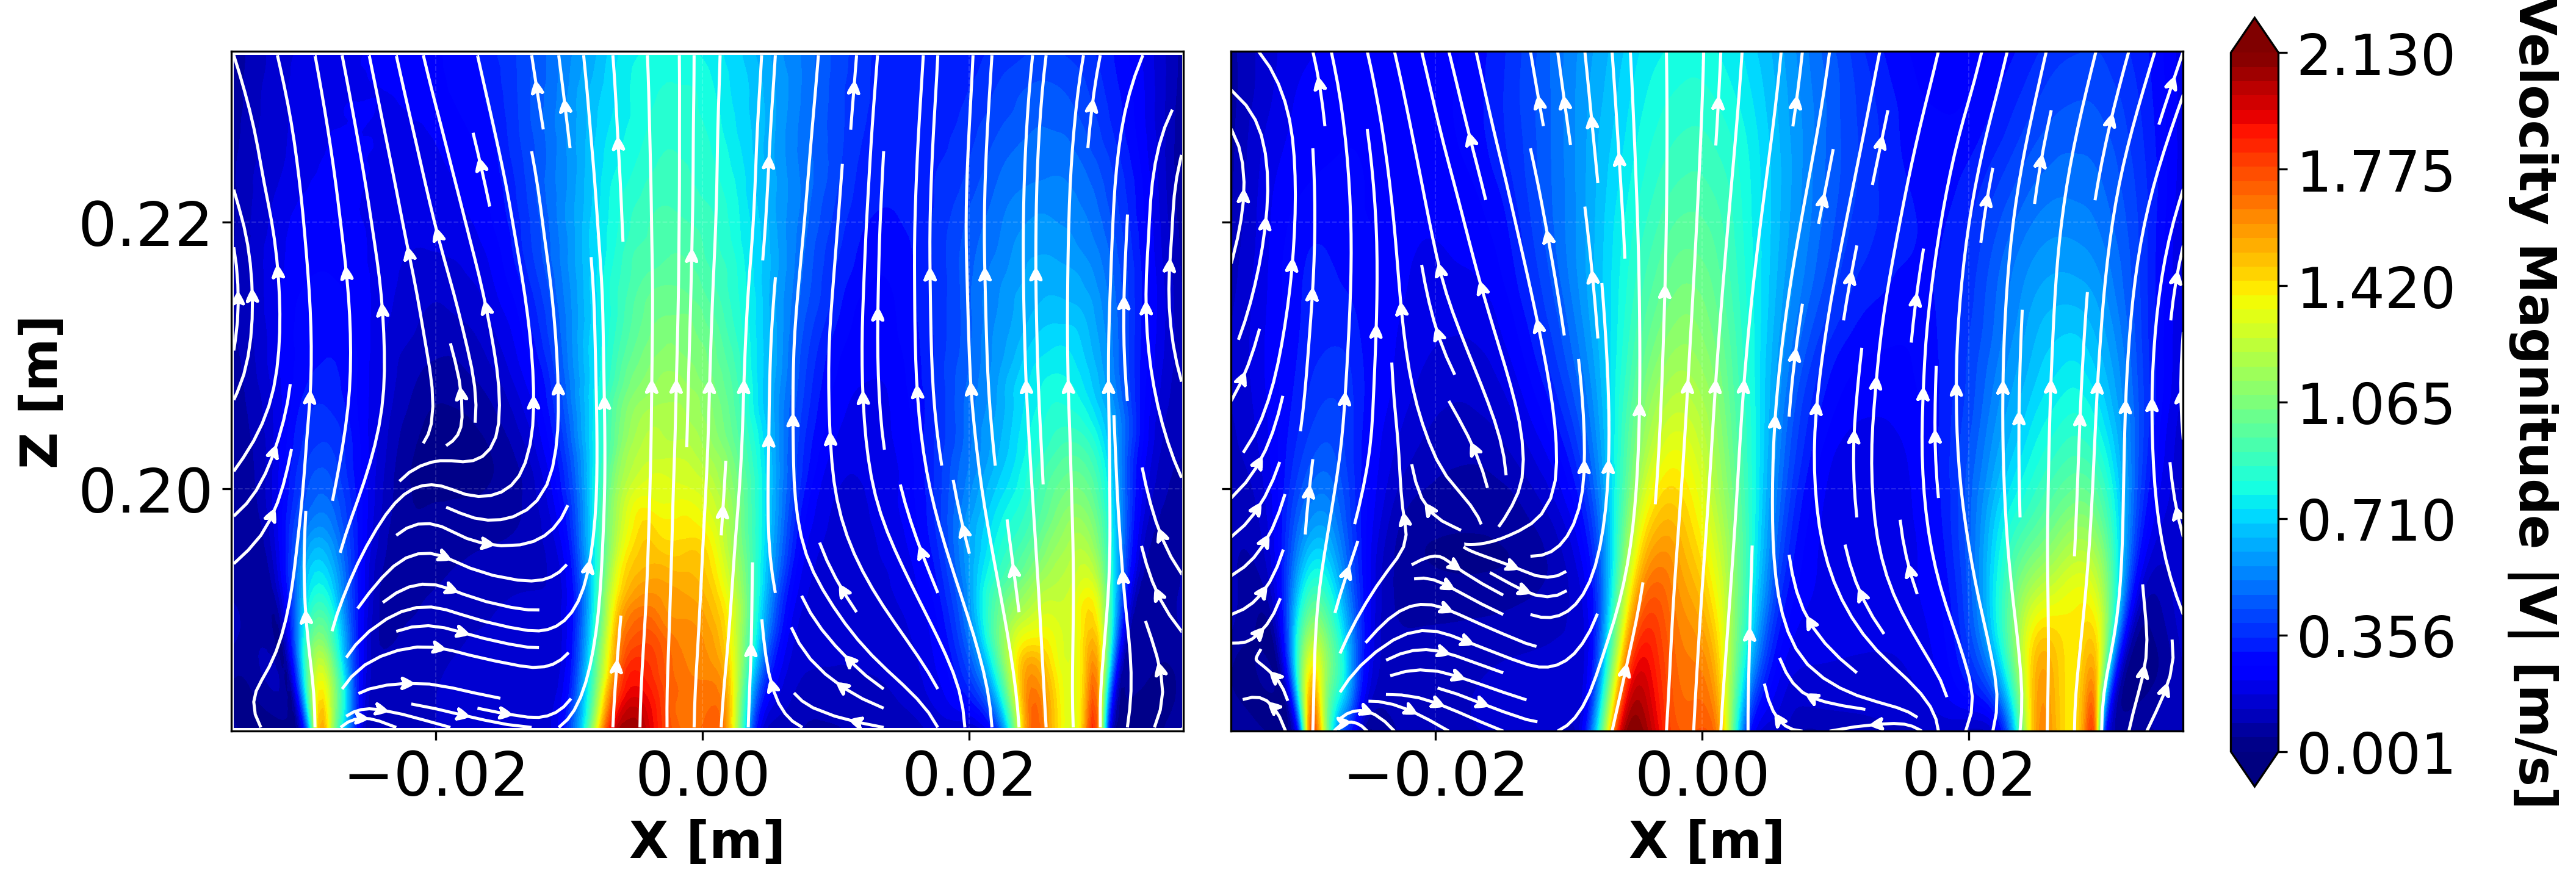
\includegraphics[width=0.95\linewidth]{30_Re_300/surface/pos3_Surface_plot.png}}\\
\subfloat[Profiles of velocity magnitude along horizontal lines]{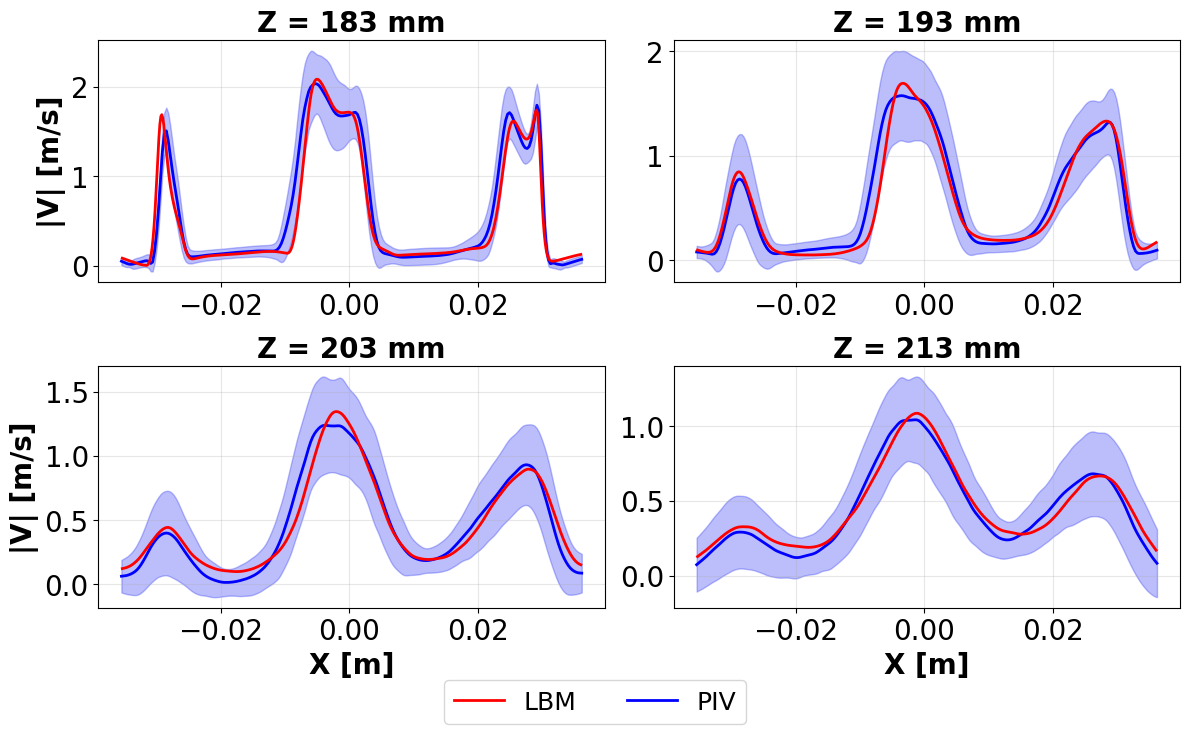
\includegraphics[width=0.95\linewidth]{30_Re_300/surface/Summary_Line_Profiles_Pos3.png}}
\caption{Validation at the freeboard for the packing with $\theta=30^\circ$ at Pos3 for Re$_p=300$: (a)~time-averaged fields of velocity magnitude with in-plane streamlines, experiment (left) vs. simulation (right); (b)~profiles of velocity magnitude across the plane at four streamwise heights, simulation (red) vs. PIV (blue) with the blue band showing $\pm1\sigma$ of the shot-to-shot velocity fluctuations in the PIV data.}
\label{fig:validation_surface_re300}
\end{figure}

\subsubsection{Comparisons Within the Packing}
\label{sec:validation:layers}

By replacing individual bars of one module by an identical but optically transparent alternative made of quartz glass bars (see~\cite{velten2026} for details), the PIV measurements also resolve the flow within the individual layers of the packing, allowing the simulation to be validated layer by layer. The complete dataset includes in-slit velocity fields and profiles for each measured layer, packing topology, Reynolds number and measurement position. To avoid redundancy and maintain focus, only representative results are presented here. Since the packing with $\theta=30^\circ$ was retained for comparisons at the freeboard, the comparisons within the packing focus now on the case $\theta=40^\circ$, for both Re$_p=100$ and $300$. Additionally, results are shown for the irregular configuration at Re$_p=100$. These choices demonstrate both the accuracy of the numerical method across different topologies and Reynolds numbers, and the distinctly different flow development associated with periodic versus irregular packing arrangements.

For the regular $40^\circ$ packing at Re$_p=100$ (Fig.~\ref{fig:validation_layers_40re100}), a good agreement is again observed between the simulated and measured fields of velocity magnitude. The velocity contours and corresponding in-plane streamlines (Fig.~\ref{fig:validation_layers_40re100}a) reproduce well the jet-recirculation structures observed in each layer. To demonstrate quantitative agreement, profiles of velocity magnitude have been extracted at different vertical positions (Fig.~\ref{fig:validation_layers_40re100}b). The simulation results of the individual layers are shown as thin coloured lines, while the experimental reference (PIV) of a single layer (L14) is shown as a thick blue line with the standard deviation band \added{(layer-to-layer spread)}\deleted{ representing velocity fluctuations} (shaded region).\remark{15}{The text names L14 as the experimental reference, while the caption of Fig.~\ref{fig:validation_layers_40re100} says ``within element L15''. Also ``thick blue line'' here vs.\ ``blue lines'' in the caption. Please make consistent.} As the experimental reference is a single layer, the simulated layers are not expected to match it exactly, and the comparison is best judged against the shaded band. The simulation accurately captures the central jet, the flanking secondary jets, and the inter-jet minima across the entire layer height. Slight remaining discrepancies are primarily confined to thin shear layers at the jet boundaries, where large velocity gradients exist and fluctuations are experimentally observed to be most intense. This is particularly visible in Fig.~\ref{fig:validation_layers_40re100}a in L16, for which one \added{of }the two jets observed close to the right wall is visibly more intense in the experiment. Looking now at Fig.~\ref{fig:validation_layers_40re100}b, this region $0<x'<0.02$\added{\,m} corresponds to very large fluctuations in time, particularly so when approaching the next element, L17; this is precisely the region where the difference between simulation and PIV is particularly large.

\begin{figure}[tbp]
\centering
\subfloat[Experimental\ (left) vs.\ simulation\ (right) contours of velocity magnitude and corresponding 2D-streamlines]{%
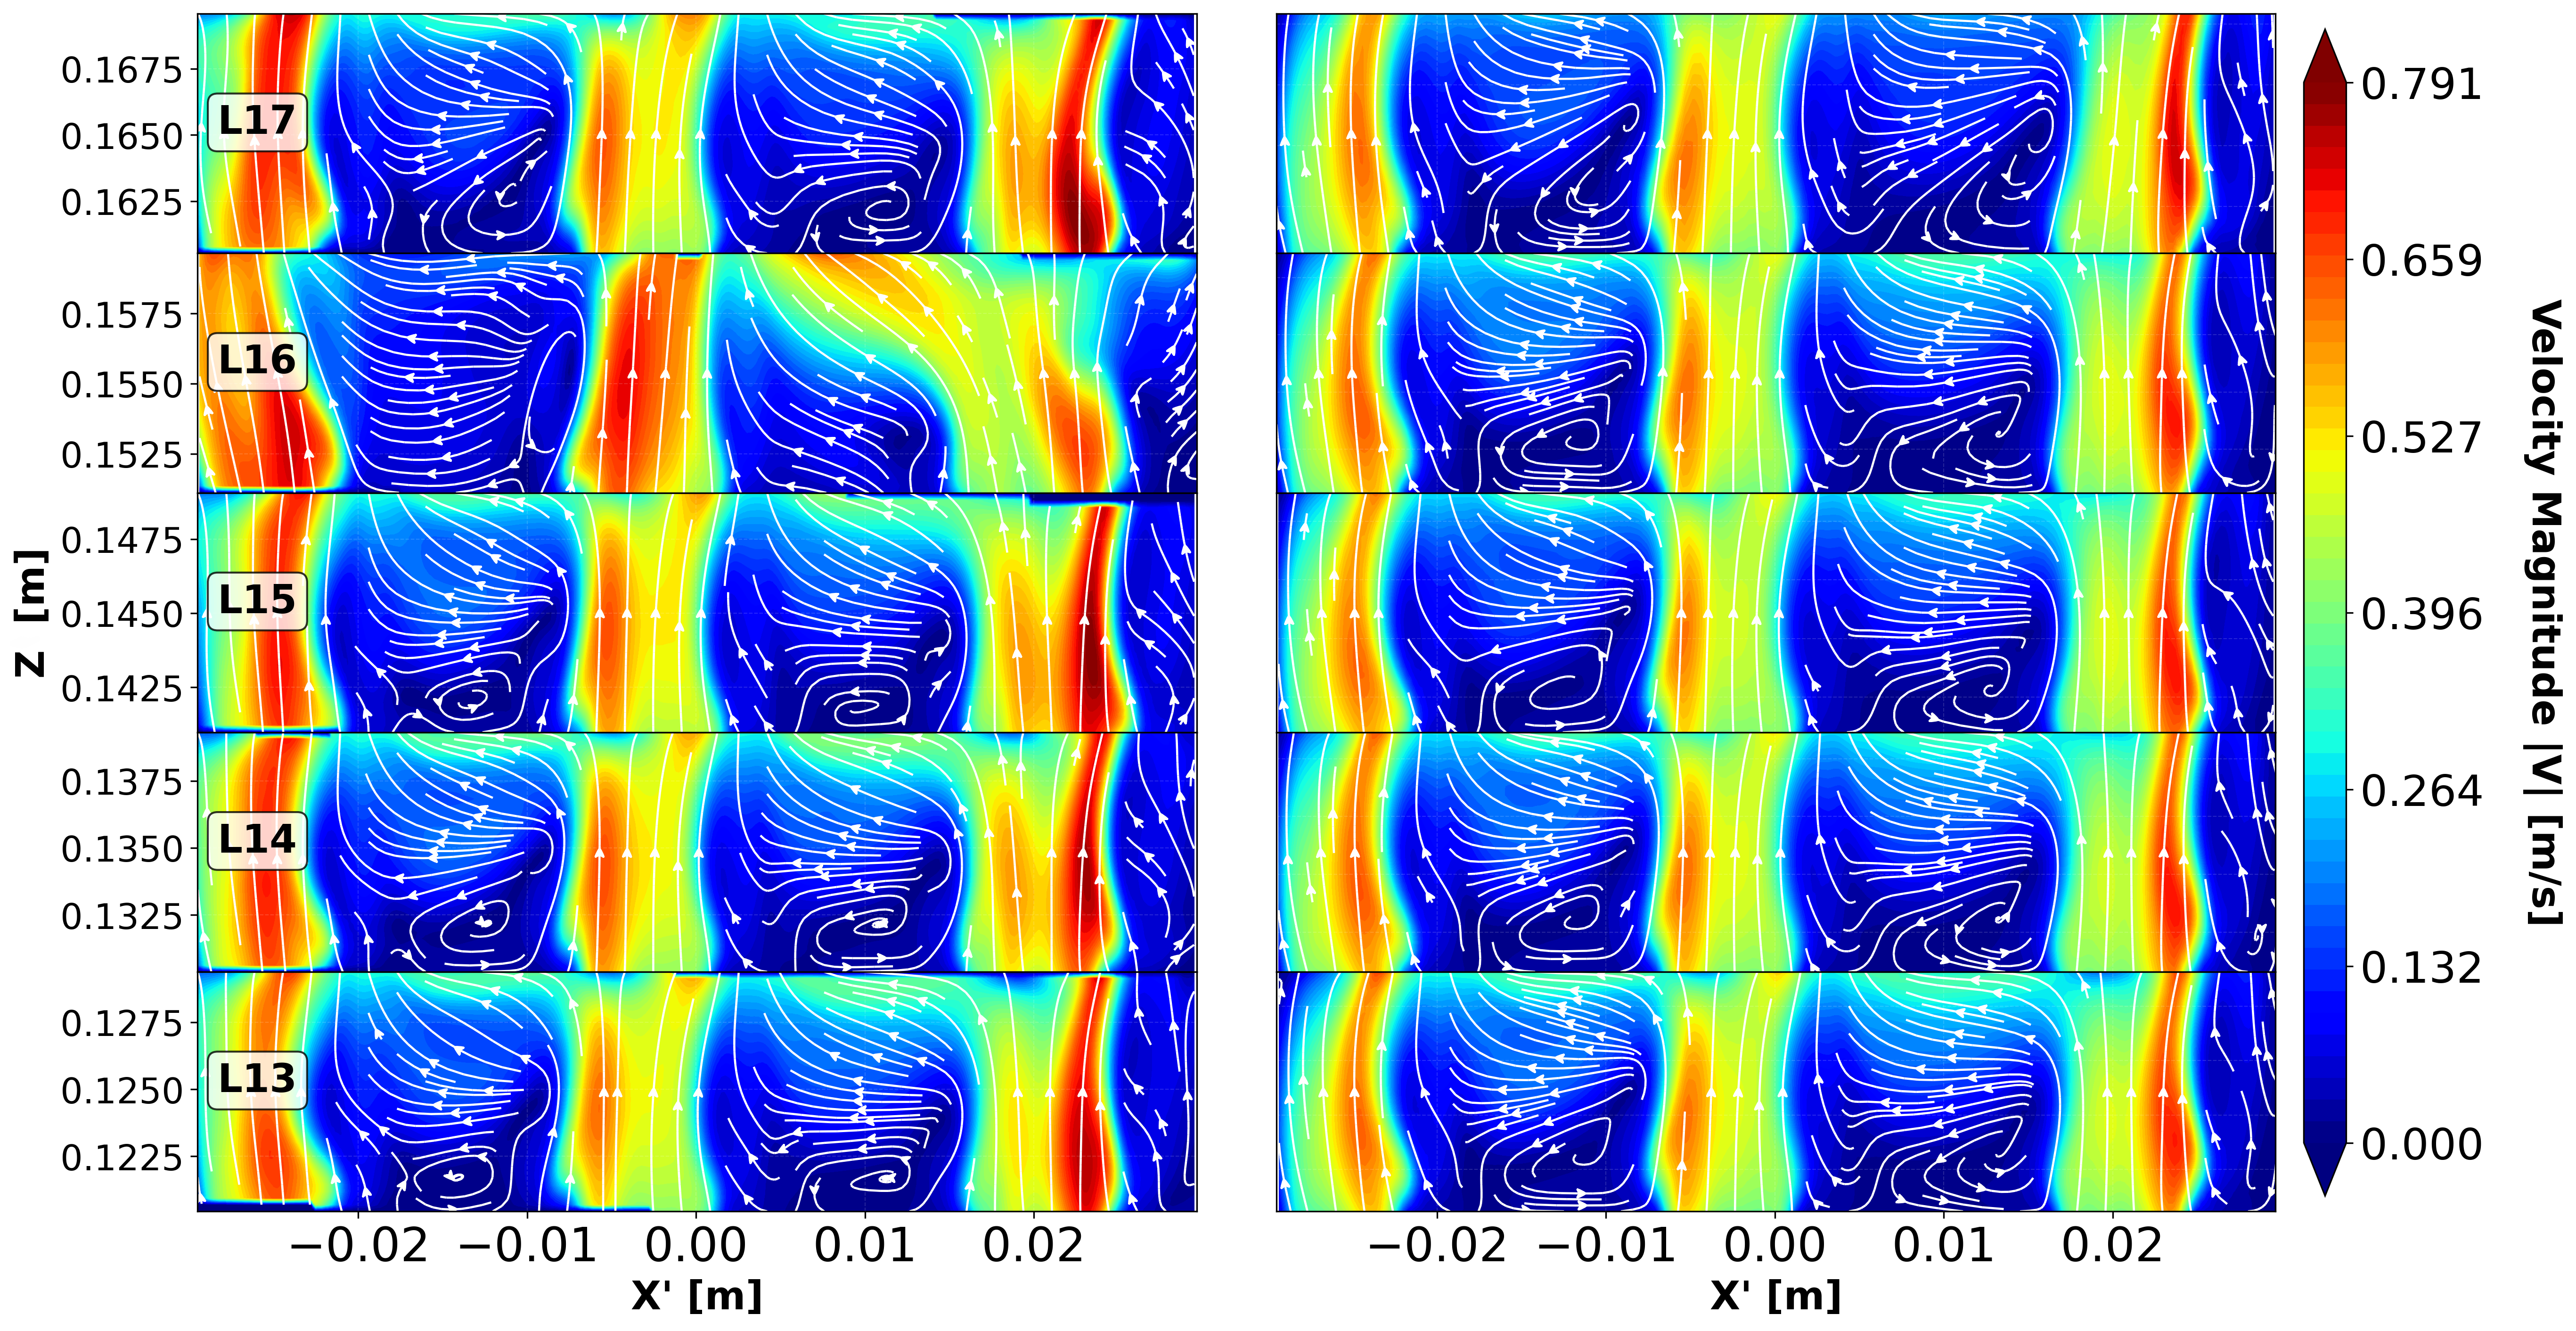
\includegraphics[width=0.78\linewidth]{40_Re_100/layers/Combined_Exp_Sim_Pos3_Re100.png}}\\
\subfloat[Profiles of velocity magnitude at different vertical positions]{%
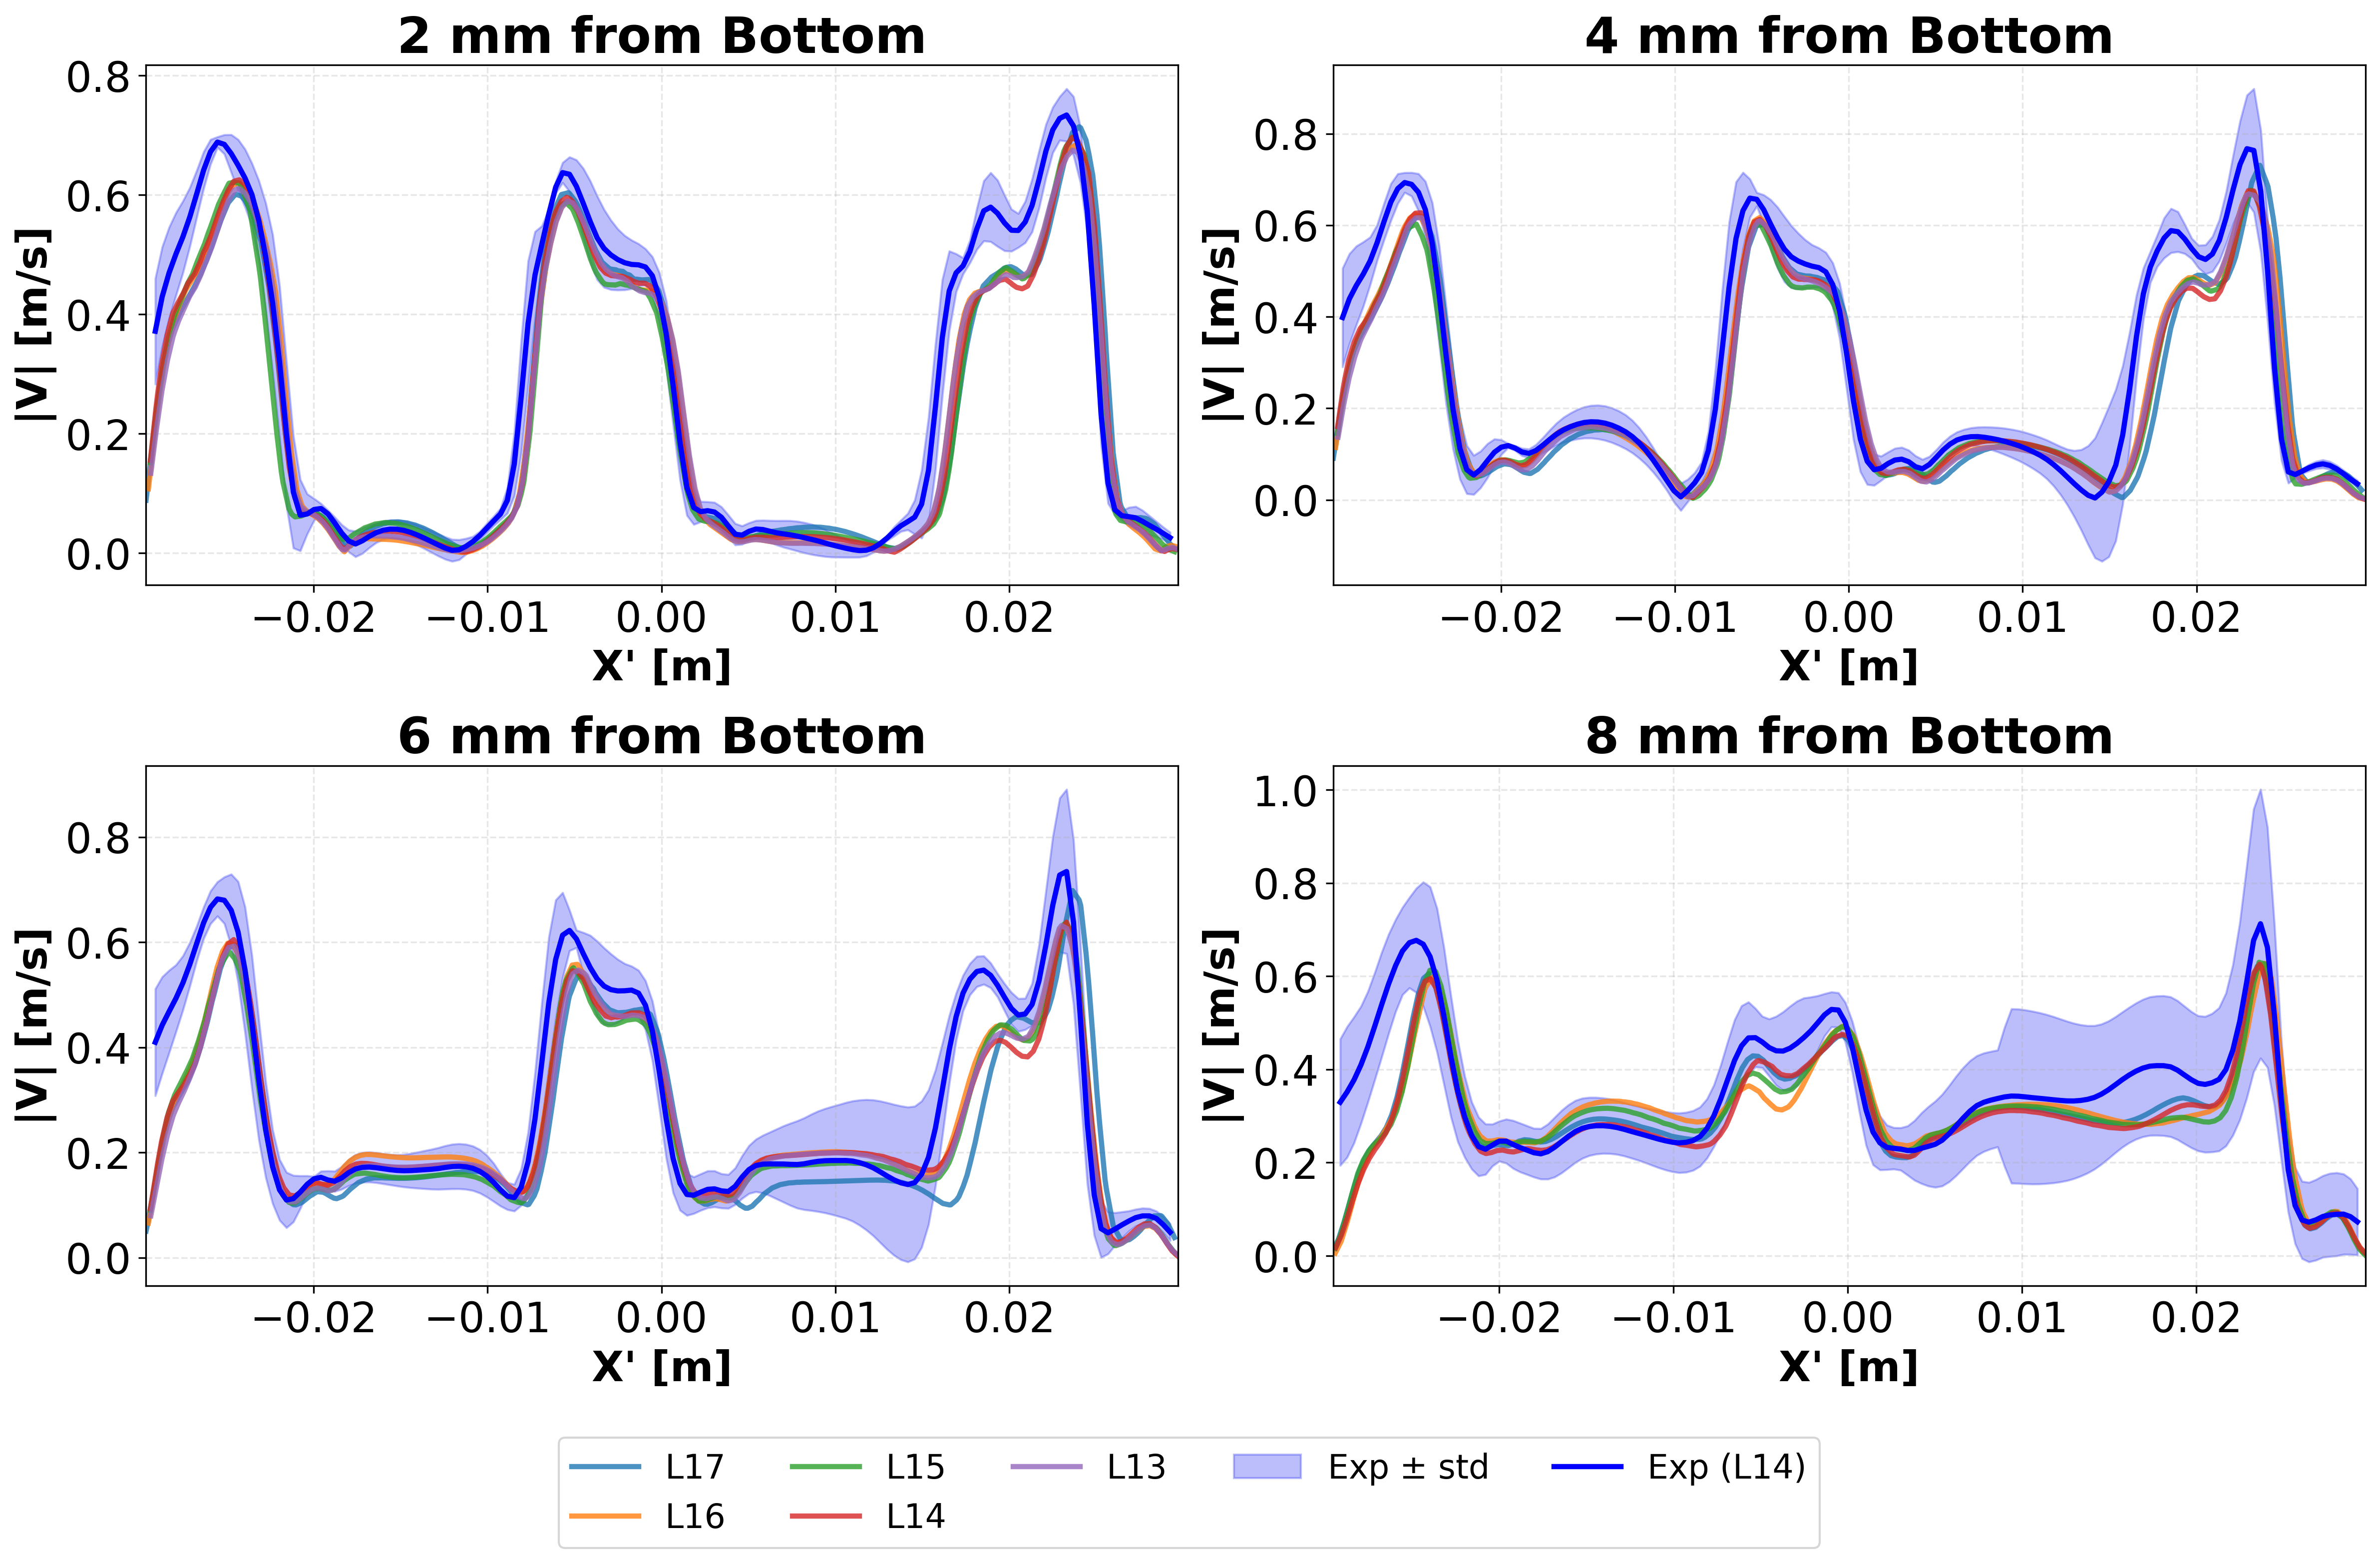
\includegraphics[width=0.8\linewidth]{40_Re_100/layers/Line_Profiles_from_Bottom_Pos3_Re100.png}}
\caption{Comparisons for the packing at $\theta=40^\circ$ and Re$_p = 100$ for Pos3 (layers L13-L17). (a)~Time-averaged contours of velocity magnitude with in-plane streamlines, experiment (left) vs.\ simulation (right). (b)~Profiles of velocity magnitude profile at different vertical positions within element L15. Simulation results are shown as thin coloured lines, experimental data as blue lines together with the layer-to-layer standard deviation (blue shaded area).}
\label{fig:validation_layers_40re100}
\end{figure}

At the higher Reynolds number Re$_p=300$ (Fig.~\ref{fig:validation_layers_40re300}), the $40^\circ$ packing leads again to a good qualitative agreement between experimental measurements and simulations across all layers. Still, it must be noticed that larger variations are observed here between different layers, both experimentally and numerically, as well as larger differences between simulation results and experiments. The contours of velocity magnitude and corresponding in-plane streamlines (Fig.~\ref{fig:validation_layers_40re300}a) reproduce the jet-recirculation structure observed in each layer. The line profiles extracted at different vertical positions (Fig.~\ref{fig:validation_layers_40re300}b) show the simulated profiles of all layers together with the experimental profile of a single layer (L14) and the standard deviation over all experimental layers. They confirm that the simulation captures the essential flow features at this higher Reynolds number, although some offsets are also visible in the peak jet velocities. Because the experimental reference is a single layer, and because layer-to-layer variations are already significant at this Reynolds number, local differences between a given simulated layer and this reference curve are expected; the comparison should therefore be judged against the spread between layers rather than against the single experimental curve. The remaining discrepancies arise possibly from the limited resolution employed in time and space. Additionally, at this higher Reynolds number, strong flow oscillations are observed also within the packing (note the very different vertical scales used in Figs.~\ref{fig:validation_layers_40re100}b and~\ref{fig:validation_layers_40re300}b), impacting the comparisons. An even longer averaging time might be needed to get fully converged data regarding mean velocity fields. Still, a large part of the numerical profiles lies within the experimental observations and the qualitative agreement is good.


\begin{figure}[tbp]
\centering
\subfloat[Experimental\ (left) vs.\ simulation\ (right) contours of velocity magnitude and corresponding 2D-streamlines]{%
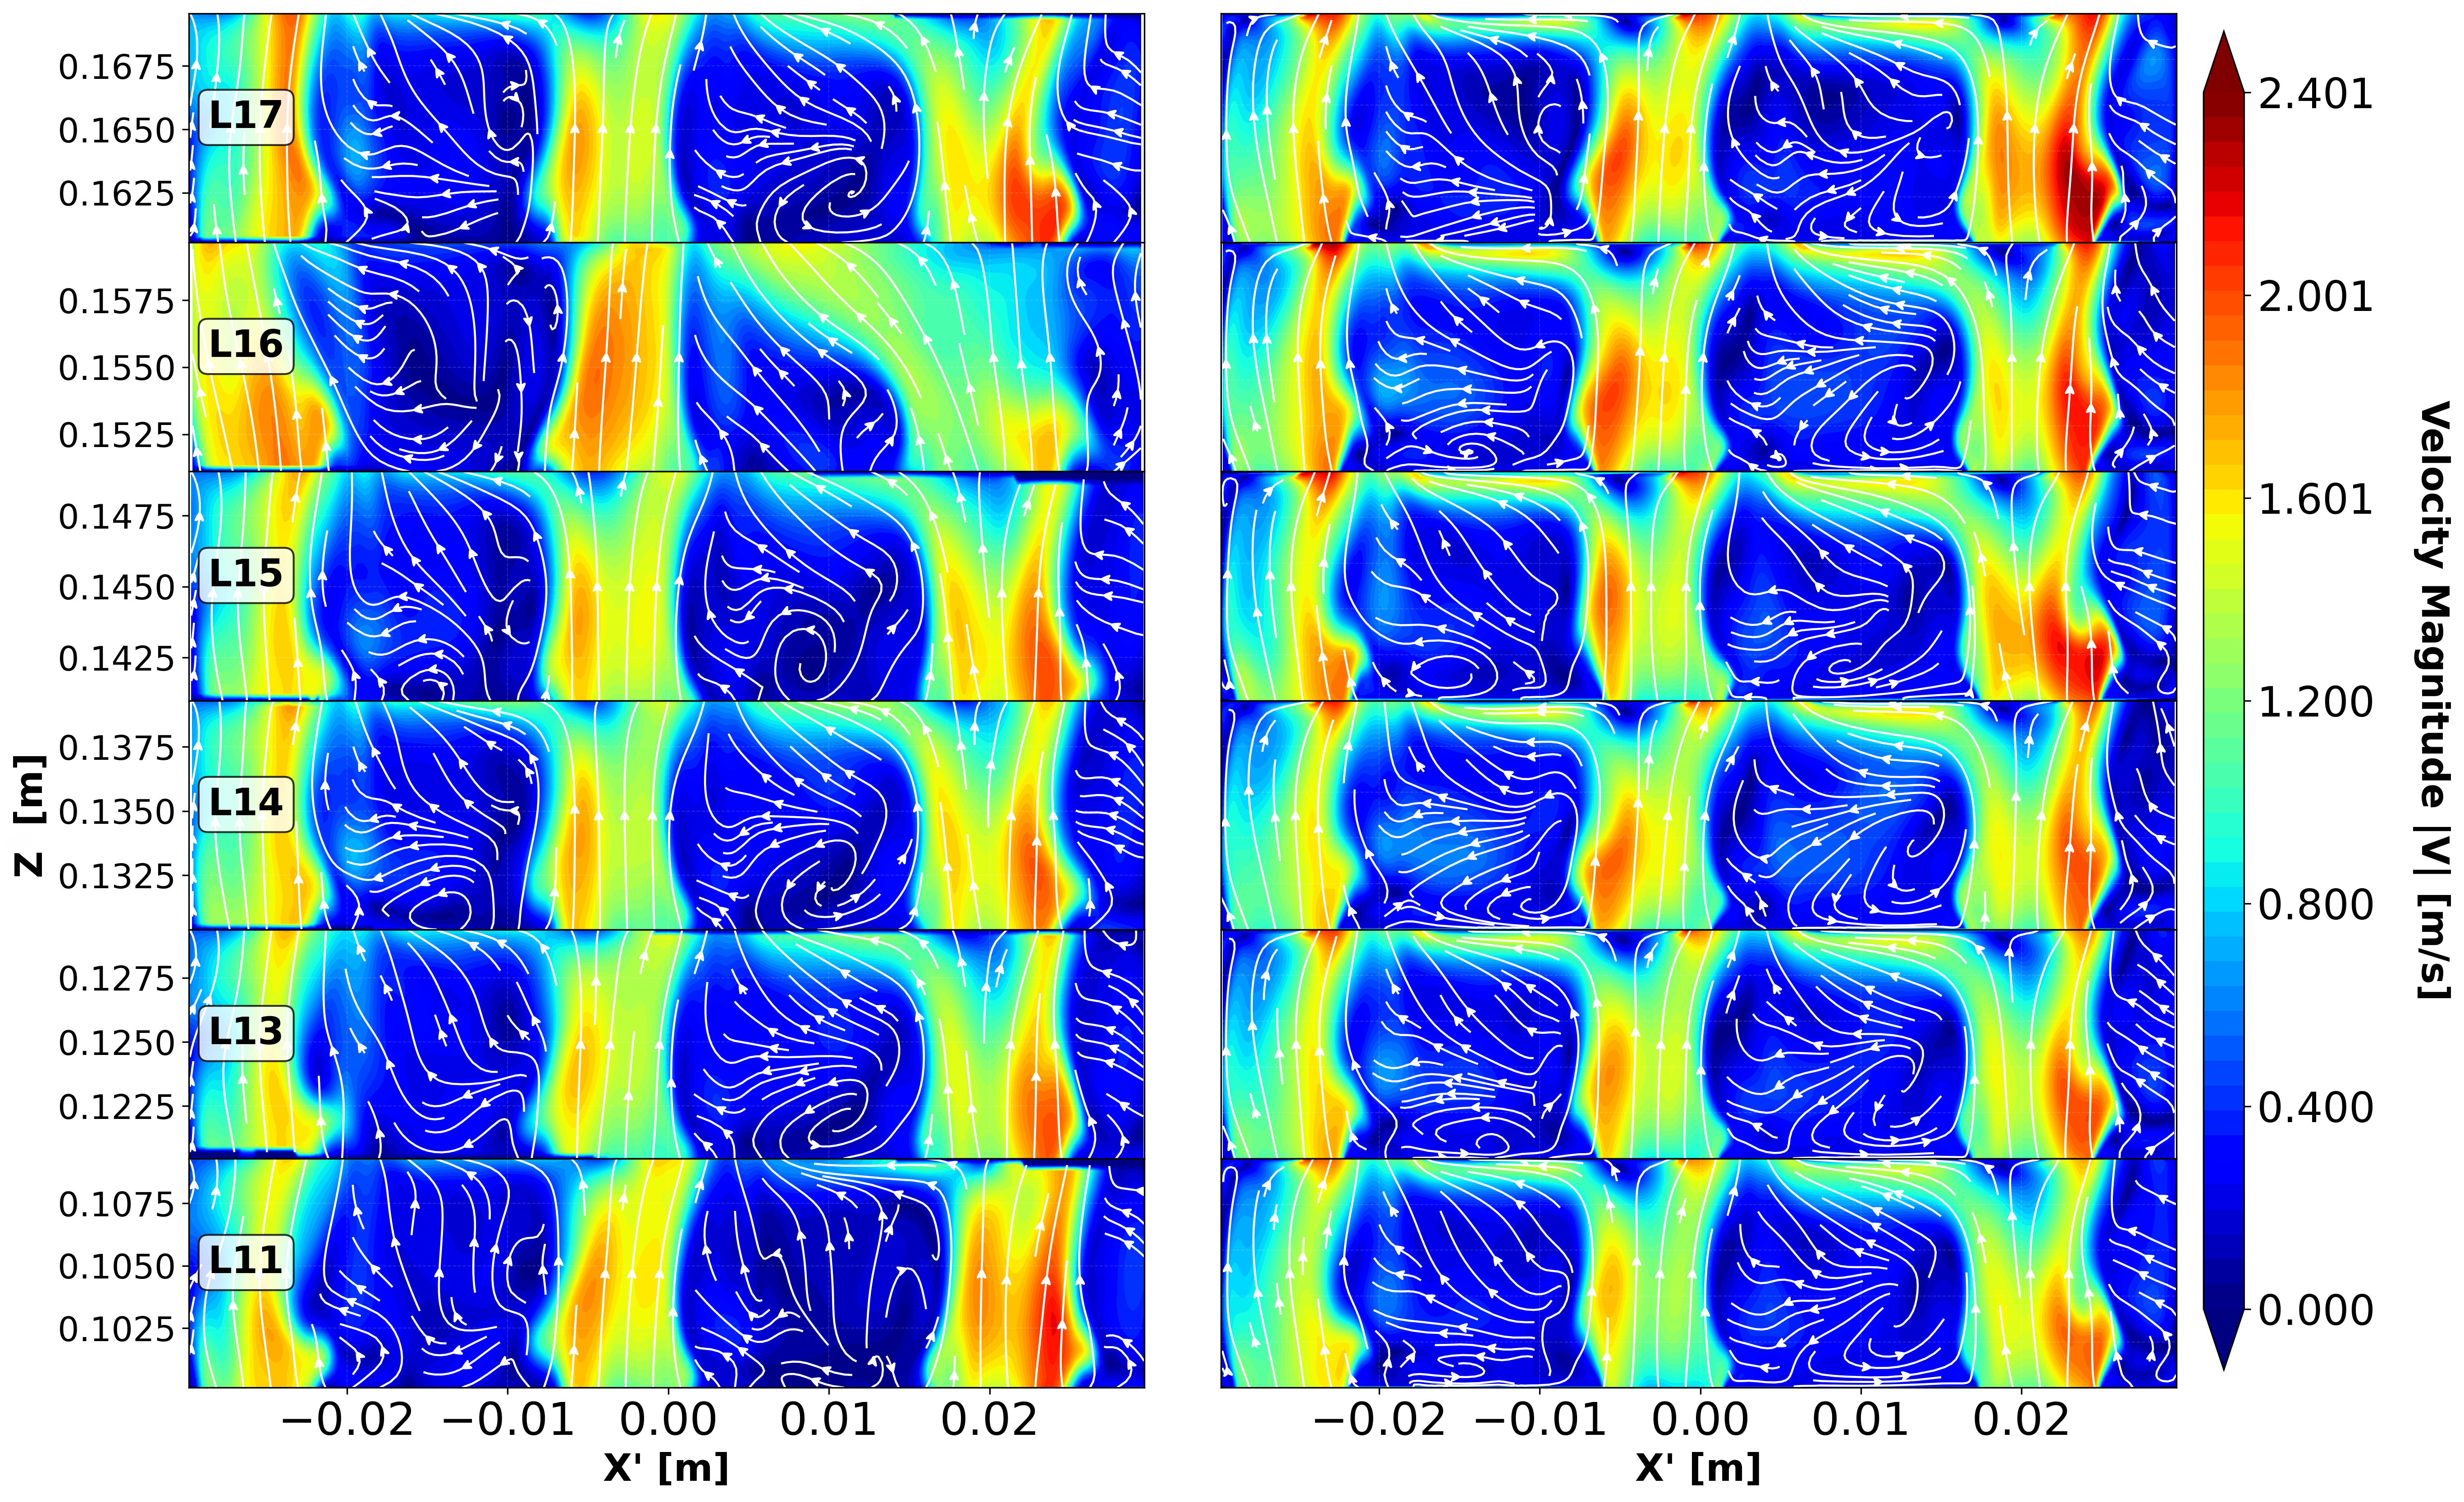
\includegraphics[width=0.78\linewidth]{40_Re_300/layers/Combined_Exp_Sim_Pos3_Re300.png}}\\
\subfloat[Profiles of velocity magnitude at different vertical positions]{%
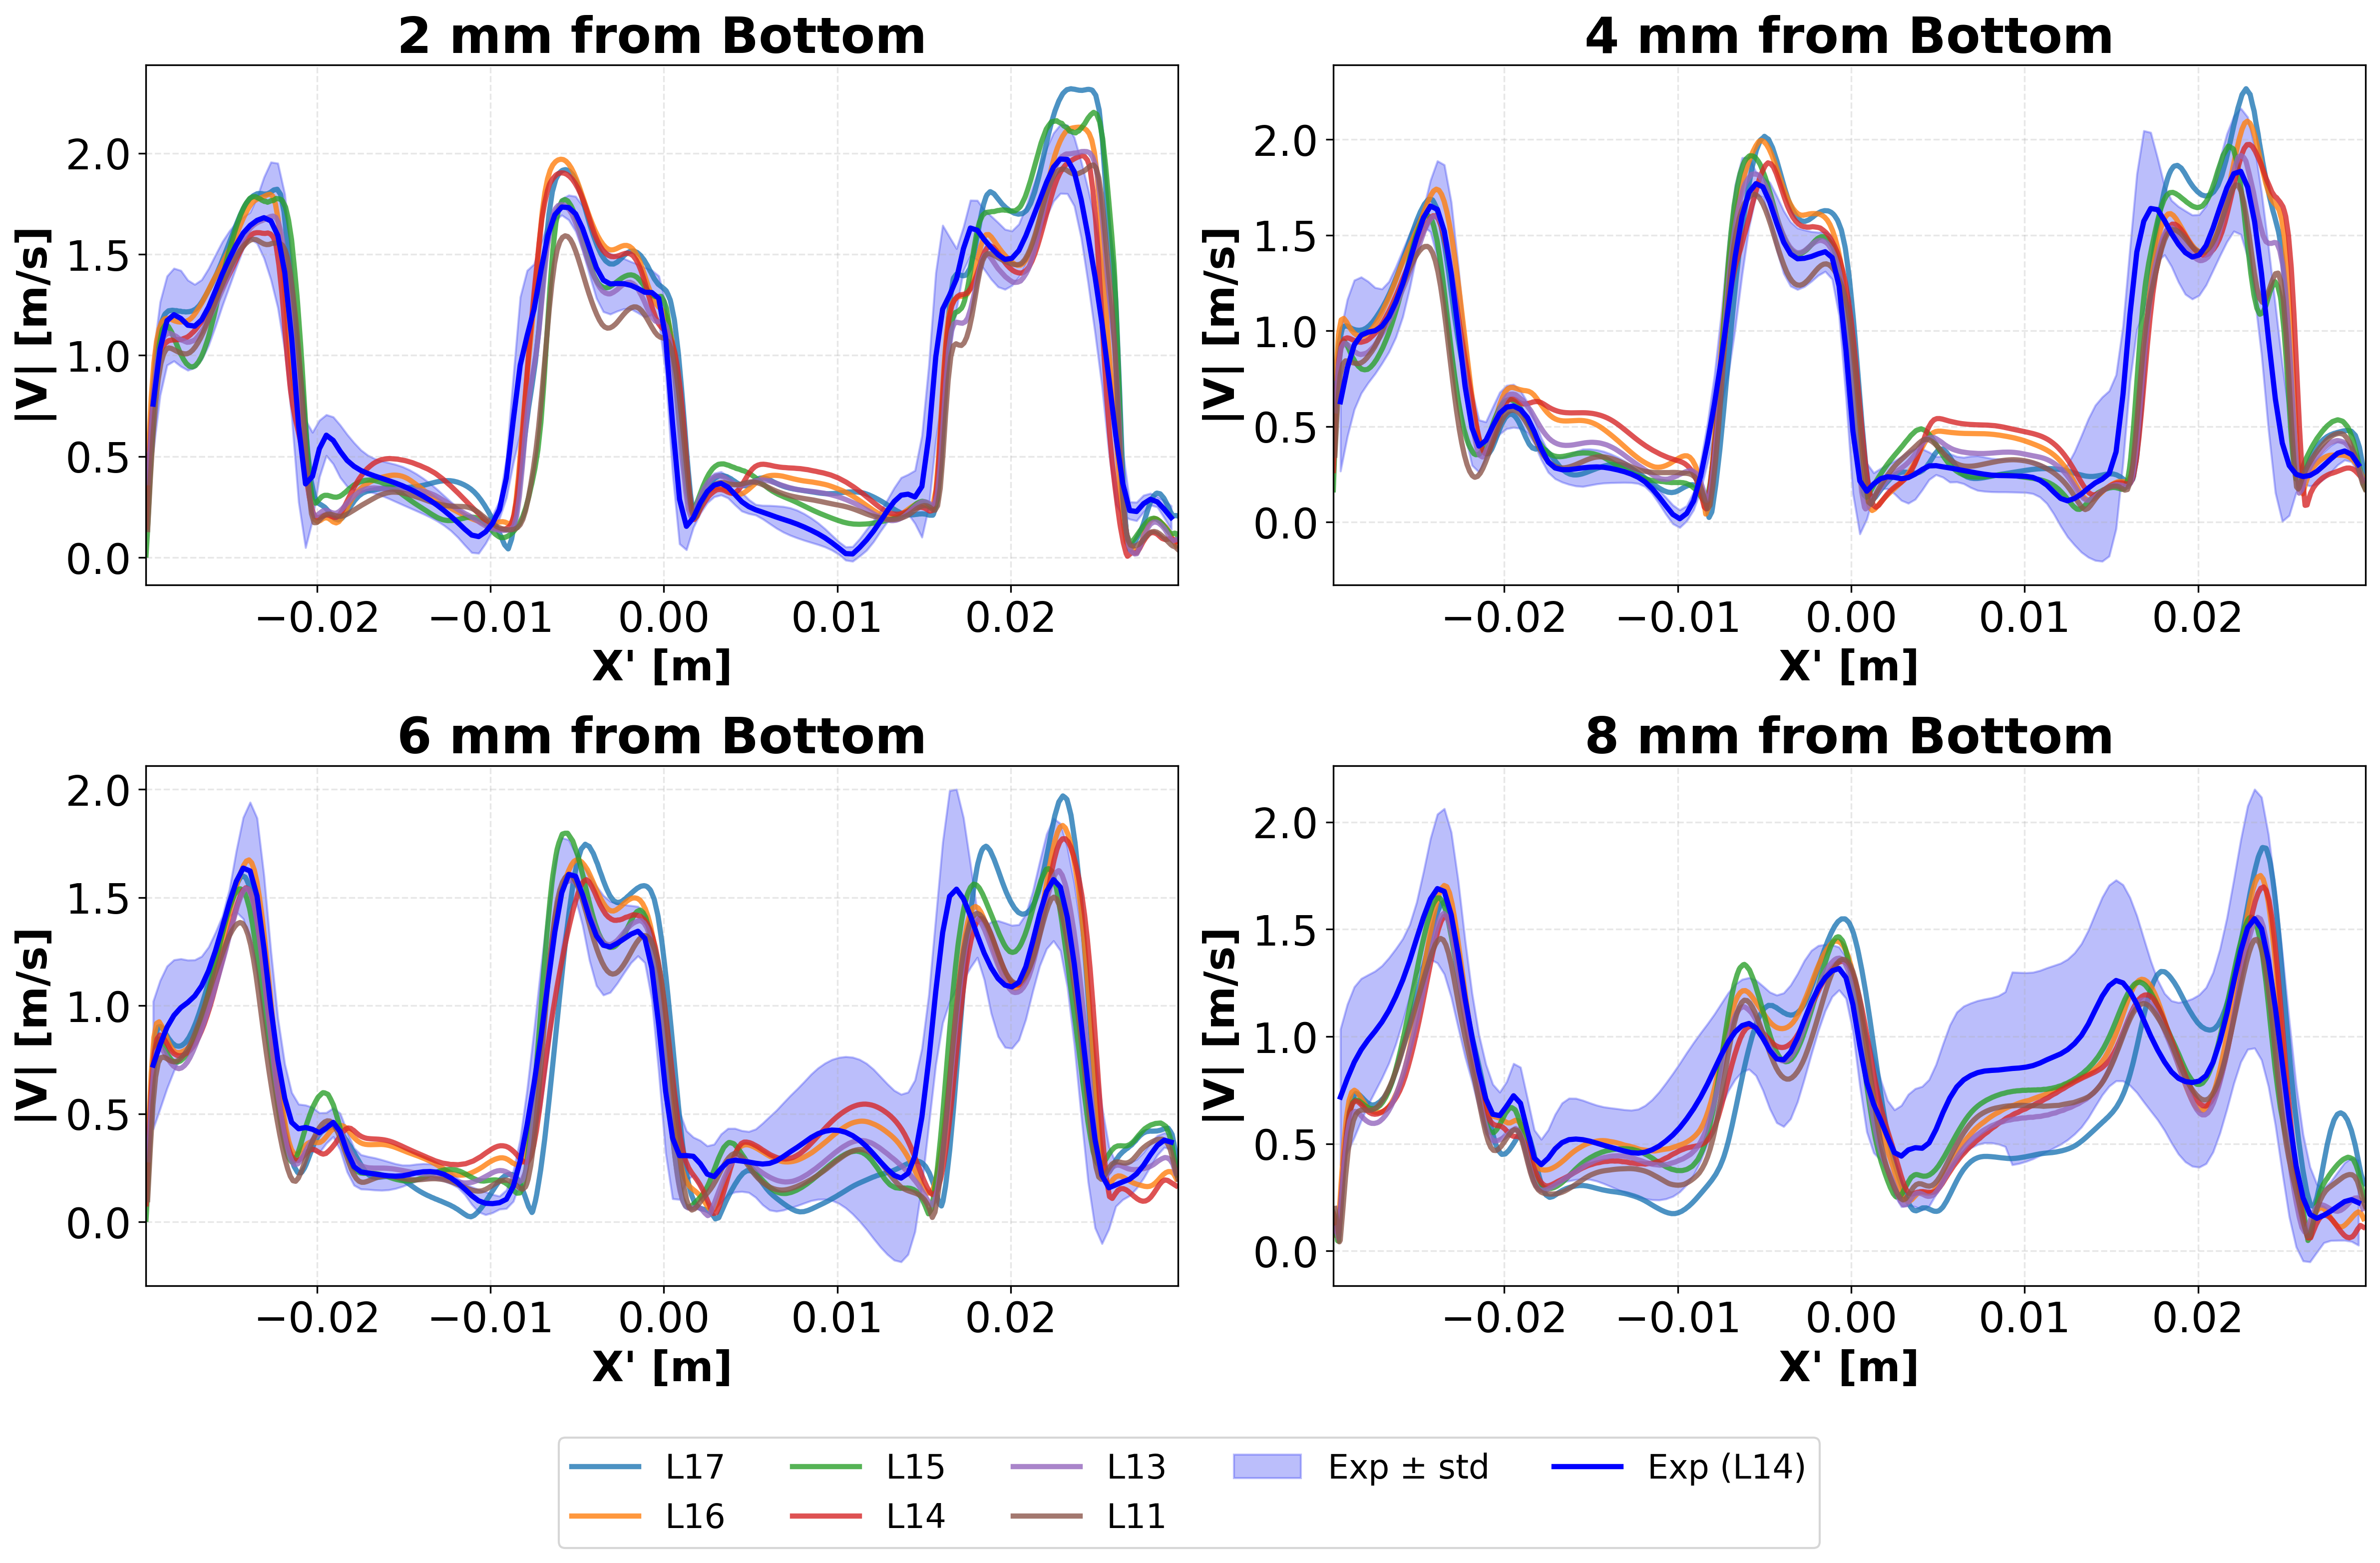
\includegraphics[width=0.8\linewidth]{40_Re_300/layers/Line_Profiles_from_Bottom_Pos3_Re300.png}}
\caption{Comparisons for the packing at $\theta=40^\circ$ and Re$_p = 300$ for Pos3 (layers L11-L17; L11 and L12 are shown in addition to L13-L17). (a)~Time-averaged contours of velocity magnitude with in-plane streamlines, experiment (left) vs.\ simulation (right); (b)~profiles of velocity magnitude at different vertical positions within the elements. Simulation results of the individual layers are shown as thin coloured lines, experimental data of layer L14 as a thick blue line, together with the standard deviation over all experimental layers (shaded area).}

\label{fig:validation_layers_40re300}
\end{figure}

Fig.~\ref{fig:validation_layers_irreg} shows the corresponding comparisons for the irregular packing, using exactly the same geometry in simulations and experiments. As expected, a fundamentally different flow behaviour is now observed. Because each layer has a unique local geometrical arrangement compared to the previous and to the following element, the corresponding jet and wake structures are also unique. For this reason, each layer is compared individually against its corresponding PIV measurements (Fig.~\ref{fig:validation_layers_irreg}b) transformed into the in-plane system with its own, layer-specific rotation angle.

The numerical model reproduces the measured flow features in every layer. The simulations mostly capture the layer-specific jet locations, jet widths, and associated recirculation regions, demonstrating that the layer-specific flow is correctly described. However, the agreement is less precise in some layers, with noticeable differences in peak velocities visible in the line profiles (Fig.~\ref{fig:validation_layers_irreg}b). We believe the origin of these discrepancies is mostly geometric. \deleted{In all periodic configurations, the repeating topology causes any small manufacturing or assembly imperfections to remain zero in the mean, disappearing statistically after a sufficient number of layers.} \added{In the irregular packing,} \deleted{Every}\added{every} layer\deleted{, however,} possesses a distinct neighbourhood which, depending on the local rotation angle, is more sensitive to assembling imperfections.\remark{16}{Each PIV comparison concerns one physical layer, whose imperfections enter directly, irrespective of the topology; the ``zero in the mean'' argument was therefore removed.} Possible geometric differences manifest most strongly in the peak jet velocities, where small differences in cross-sectional area can shift noticeably the peak magnitude, even if the overall flow pattern, jet locations, and recirculation zones remain well-captured.\deleted{ The numerical dissipation of the second-order scheme discussed above may add a small contribution by slightly lowering narrow jet peaks.} Additionally, long meandering channels occur in some layers, whereas much more frequent and stronger flow re-directions between elements occur in others. Such structures are more sensitive to minute geometric differences between simulations and experiments, so larger discrepancies are expected there.

Note that the shaded bands in Fig.~\ref{fig:validation_layers_irreg}b show the shot-to-shot standard deviation of the PIV velocity components, projected onto the velocity magnitude, for each individual layer. They are barely visible because this fluctuation level is only about $1$-$2\%$ of $|V|$ ($\approx 0.004\,\mathrm{m/s}$), and increases noticeably only in the thin shear layers bordering the jets. This level is similar to that of the periodic $40^\circ$ packing at the same Reynolds number. It must not be compared with the bands in Figs.~\ref{fig:validation_layers_40re100}b and~\ref{fig:validation_layers_40re300}b, which show the layer-to-layer spread of the time-averaged profiles, a different quantity that is not meaningful for the irregular packing, in which each layer is expected to differ.

The pronounced differences now observed between the velocity profiles in the different layers from L13 to L17 shown in Fig.~\ref{fig:validation_layers_irreg}b provide direct evidence that flow locking is absent in the irregular topology, as discussed in more detail in the next section.

\begin{figure}[tbp]
\centering
\subfloat[Experimental\ (left) vs.\ simulation\ (right) contours of velocity magnitude and corresponding 2D-streamlines]{%
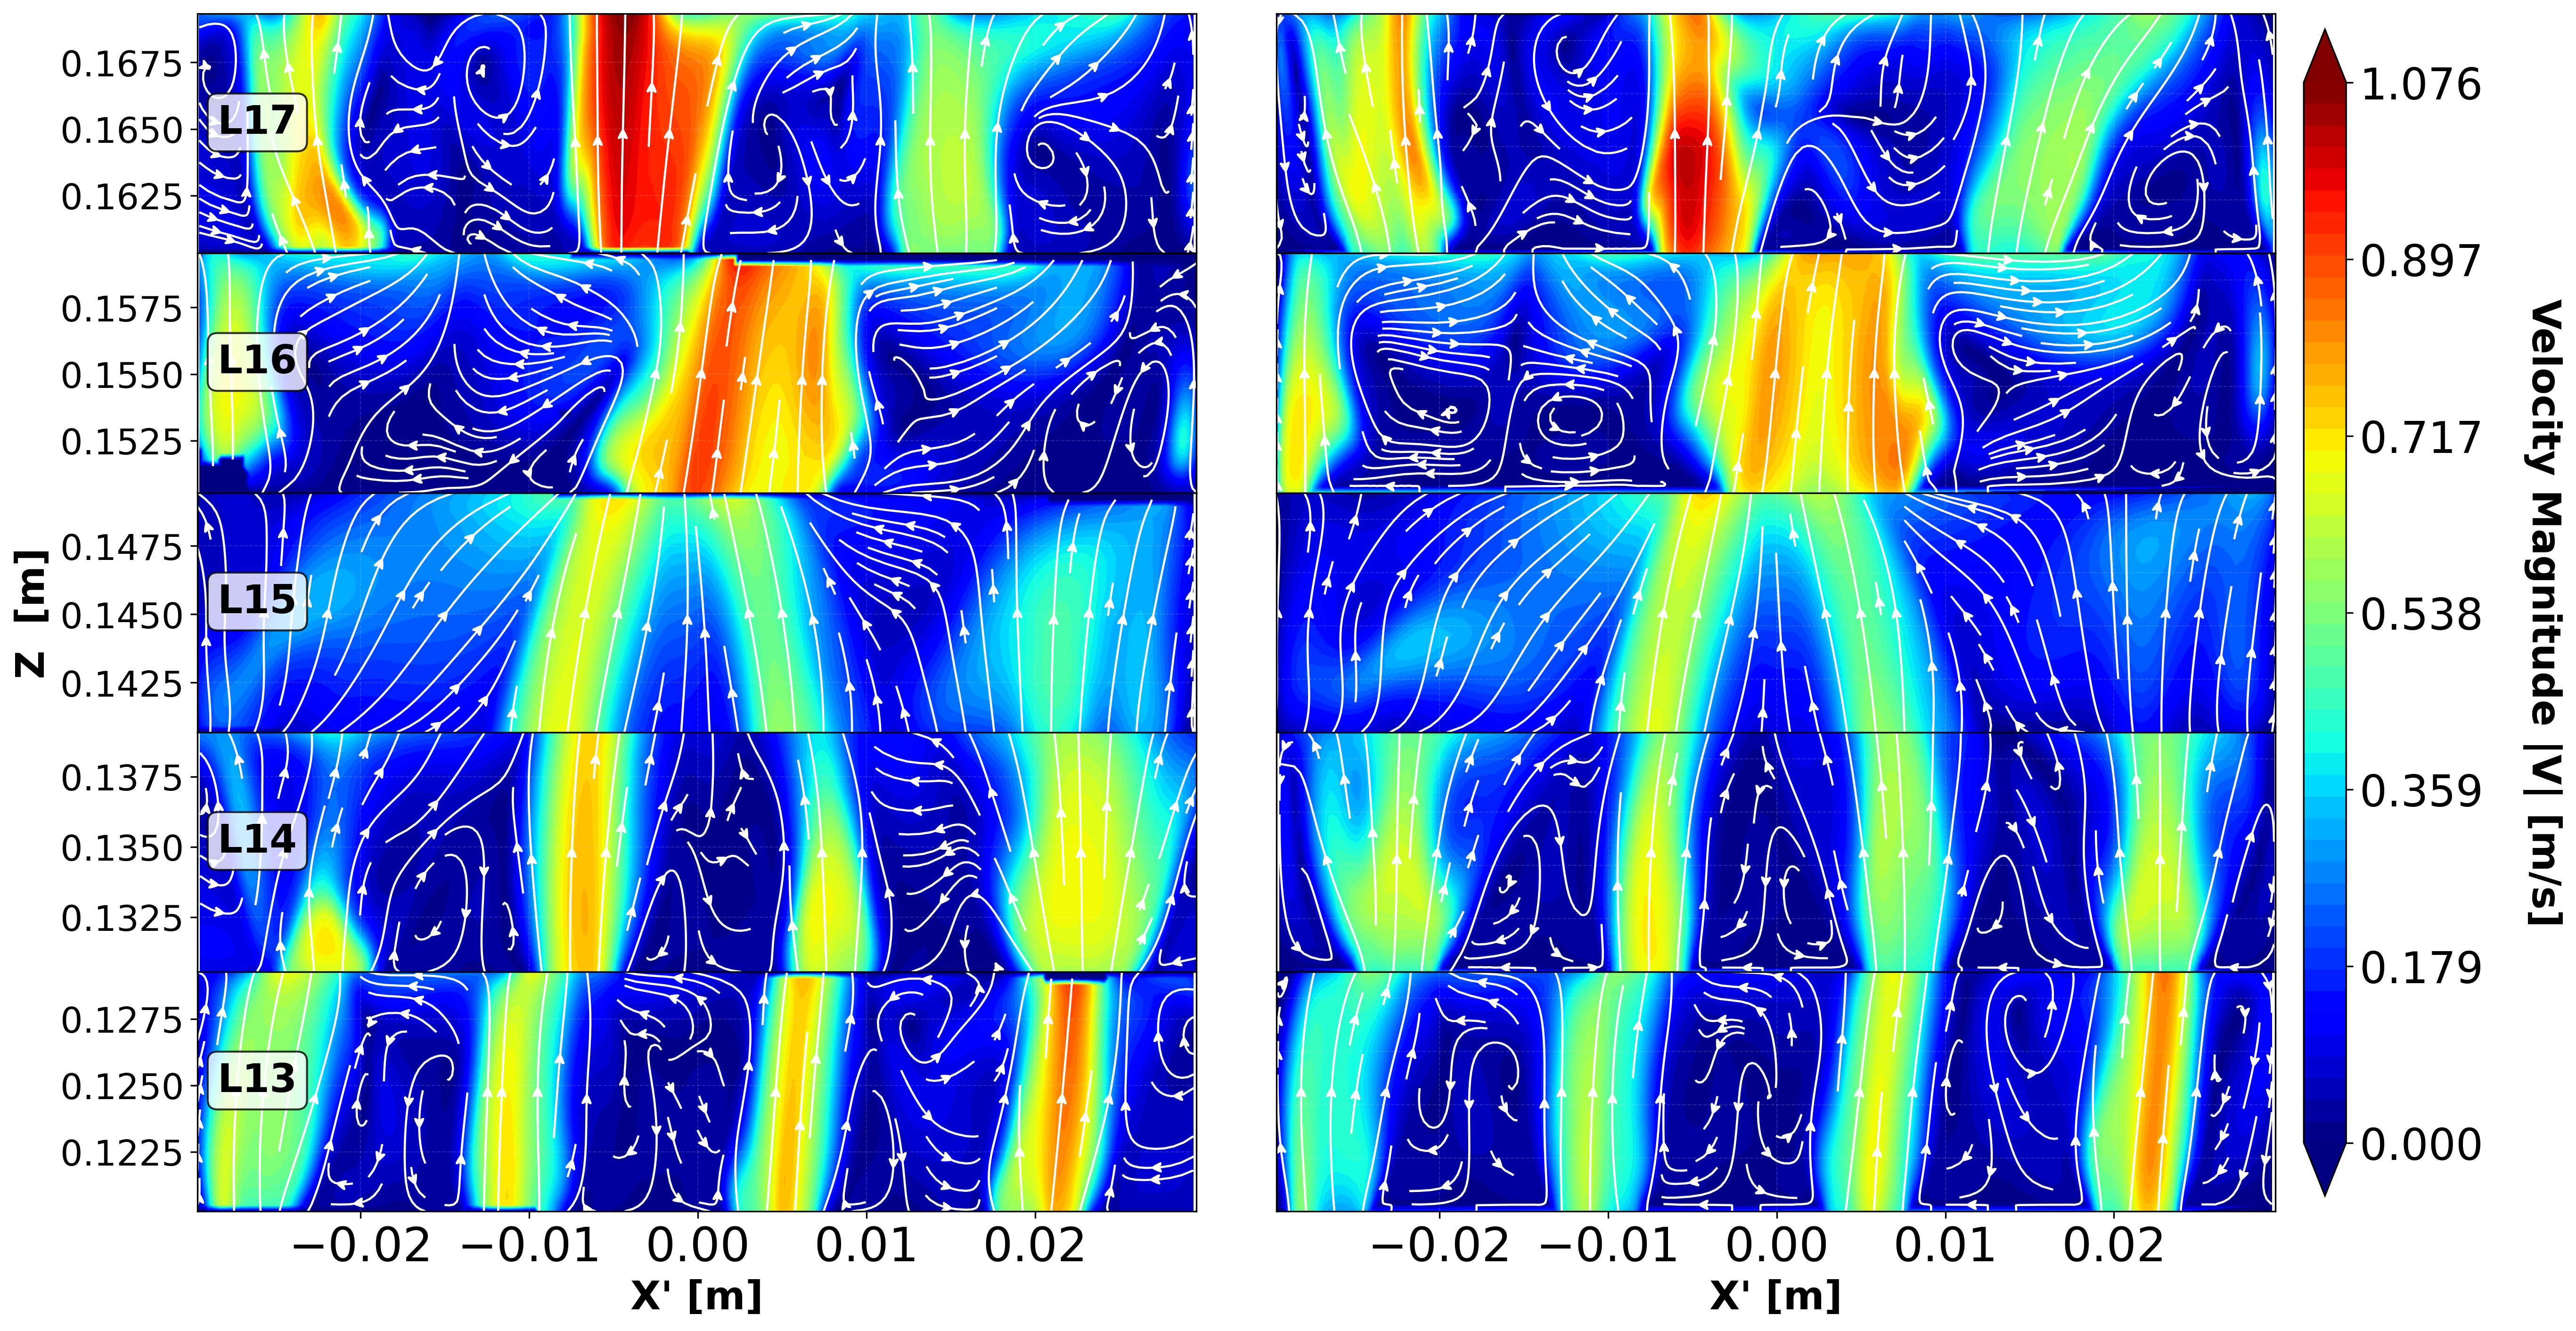
\includegraphics[width=0.9\linewidth]{irregular_Re_100/layers/Combined_Exp_Sim_Pos3_Re100.png}}\\
\subfloat[Horizontal profiles at a height of $2\,\mathrm{mm}$ within each element, simulation (red) vs.\ PIV (blue)]{%
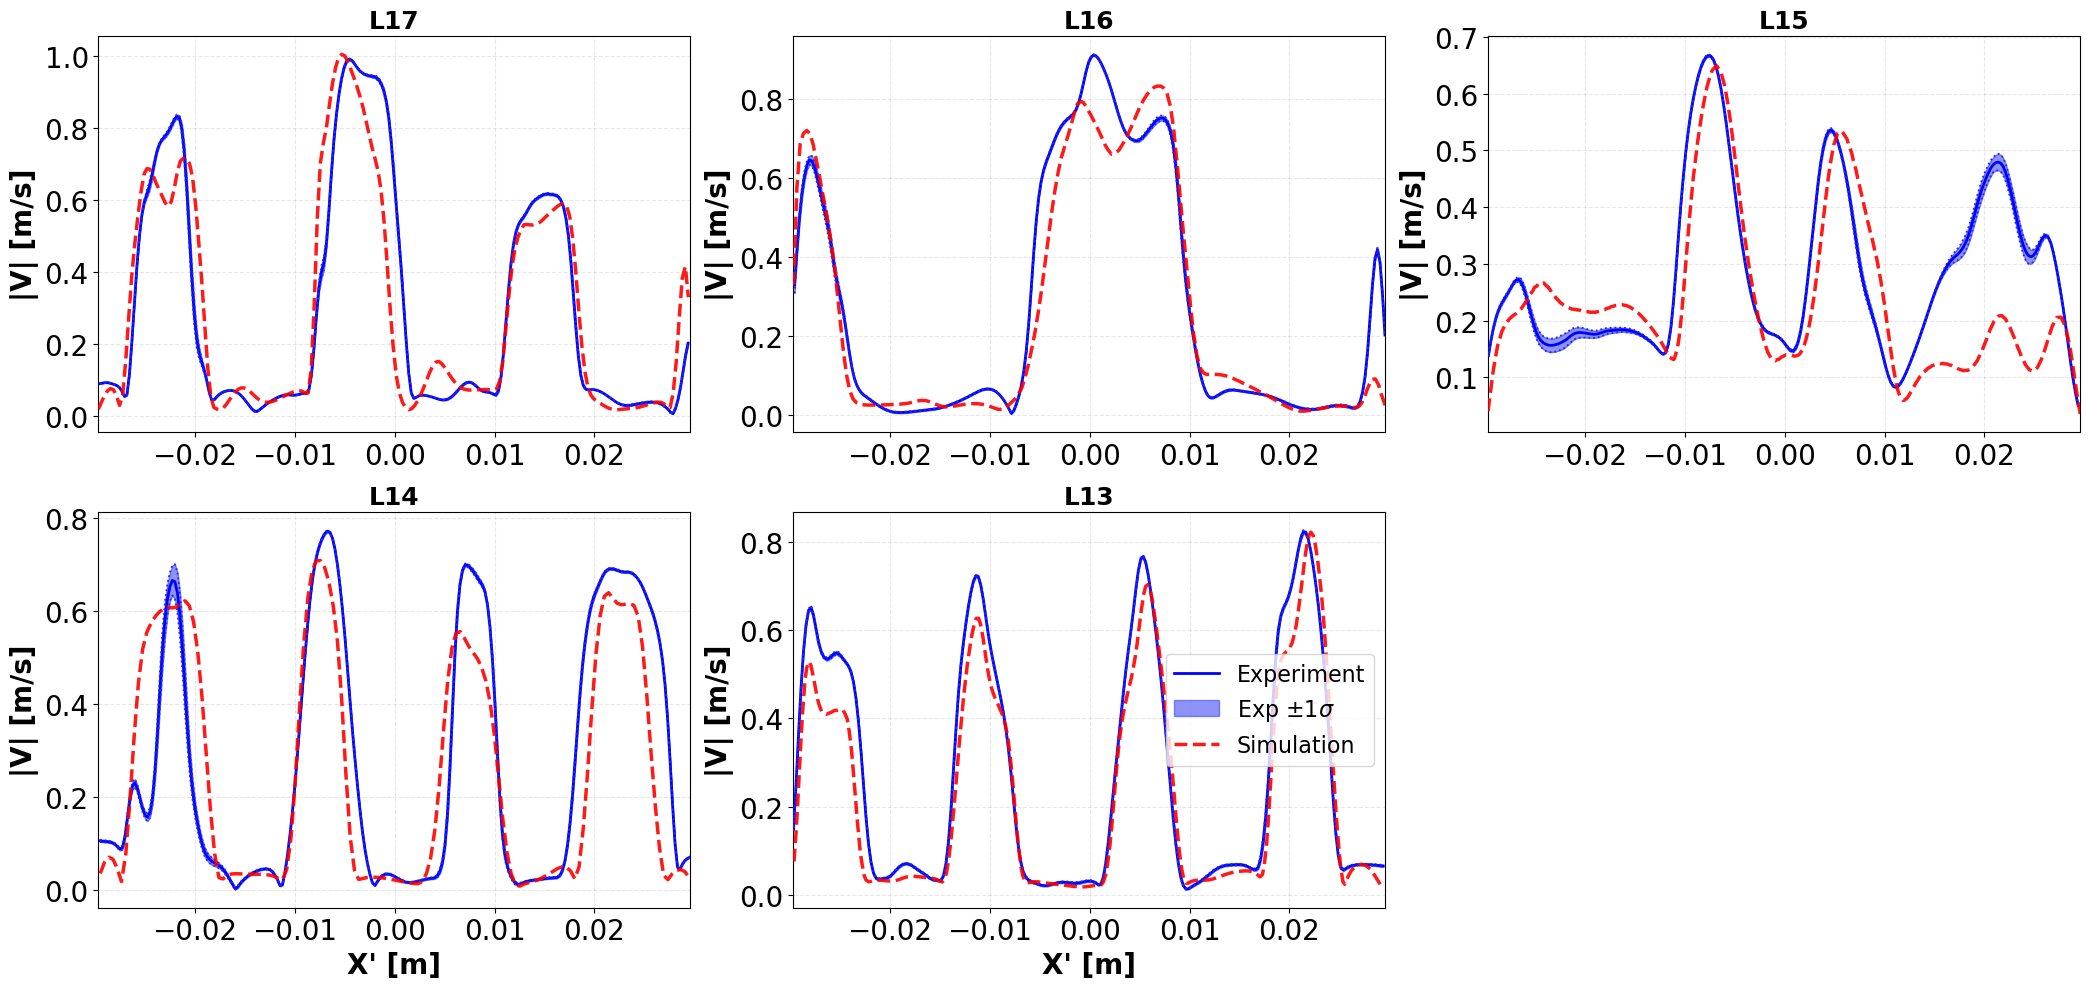
\includegraphics[width=0.9\linewidth]{irregular_Re_100/layers/Layer_Comparison_2mm_Pos3_Re100.png}}
\caption{Comparisons for the irregular packing at Re$_p = 100$ for Pos3 (layers L13-L17). (a)~Time-averaged contours of velocity magnitude with in-plane streamlines, experiment (left) vs.\ simulation (right); (b)~profiles of velocity magnitude at a height of $2\,\mathrm{mm}$ within each element, simulation (red, dashed) vs.\ PIV, (blue line for the time average, light-blue band for $\pm1\sigma$ of the shot-to-shot velocity fluctuations) for each individual layer. All results are shown in the in-plane coordinate system.}
\label{fig:validation_layers_irreg}
\end{figure}

\subsection{Flow Locking Framework}
\label{sec:locking}

This final section quantifies flow locking, which previous work~\cite{velten2026} had only observed qualitatively for $\theta=$const., without quantification or any study of the dependence on topology. Its practical relevance is that, if the developed flow repeats over each geometric period, the complete bed could be represented in numerical simulations by one or a few periodic modules as a representative elementary volume~\cite{ou2024parameter,patankar1977periodic}, which would allow reduced-order modelling in space, similar to the recurrence CFD approach introduced in time~\cite{lichtenegger2016recurrence}. \added{For a constant rotation angle, the screw symmetry discussed in Sec.~\ref{sec:geometry} even suggests that a single layer with rotate-and-shift periodic boundary conditions could suffice.}

A perfectly locked flow collapses onto a single repeating pattern, identical in each element, whereas the irregular packing, whose angles $\theta_i$ are chosen randomly, serves as a control without any expected periodicity. Figs.~\ref{fig:velocity_fields_30} and~\ref{fig:line_profiles_topology} illustrate this qualitatively. For $\theta=30^\circ$ the developed layers become nearly indistinguishable, each showing the same central jet and symmetric slit jets; only L03 differs slightly, since the flow is not yet fully established at this early level. Layer-to-layer variability increases for Re$_p=300$ (not shown in the interest of space) owing to the onset of stronger flow instabilities. In the irregular packing (Fig. ~\ref{fig:line_profiles_topology} c), no collapse is observed. The locking order parameter is now used to quantify these observations.

\begin{figure}[tbp]
\centering
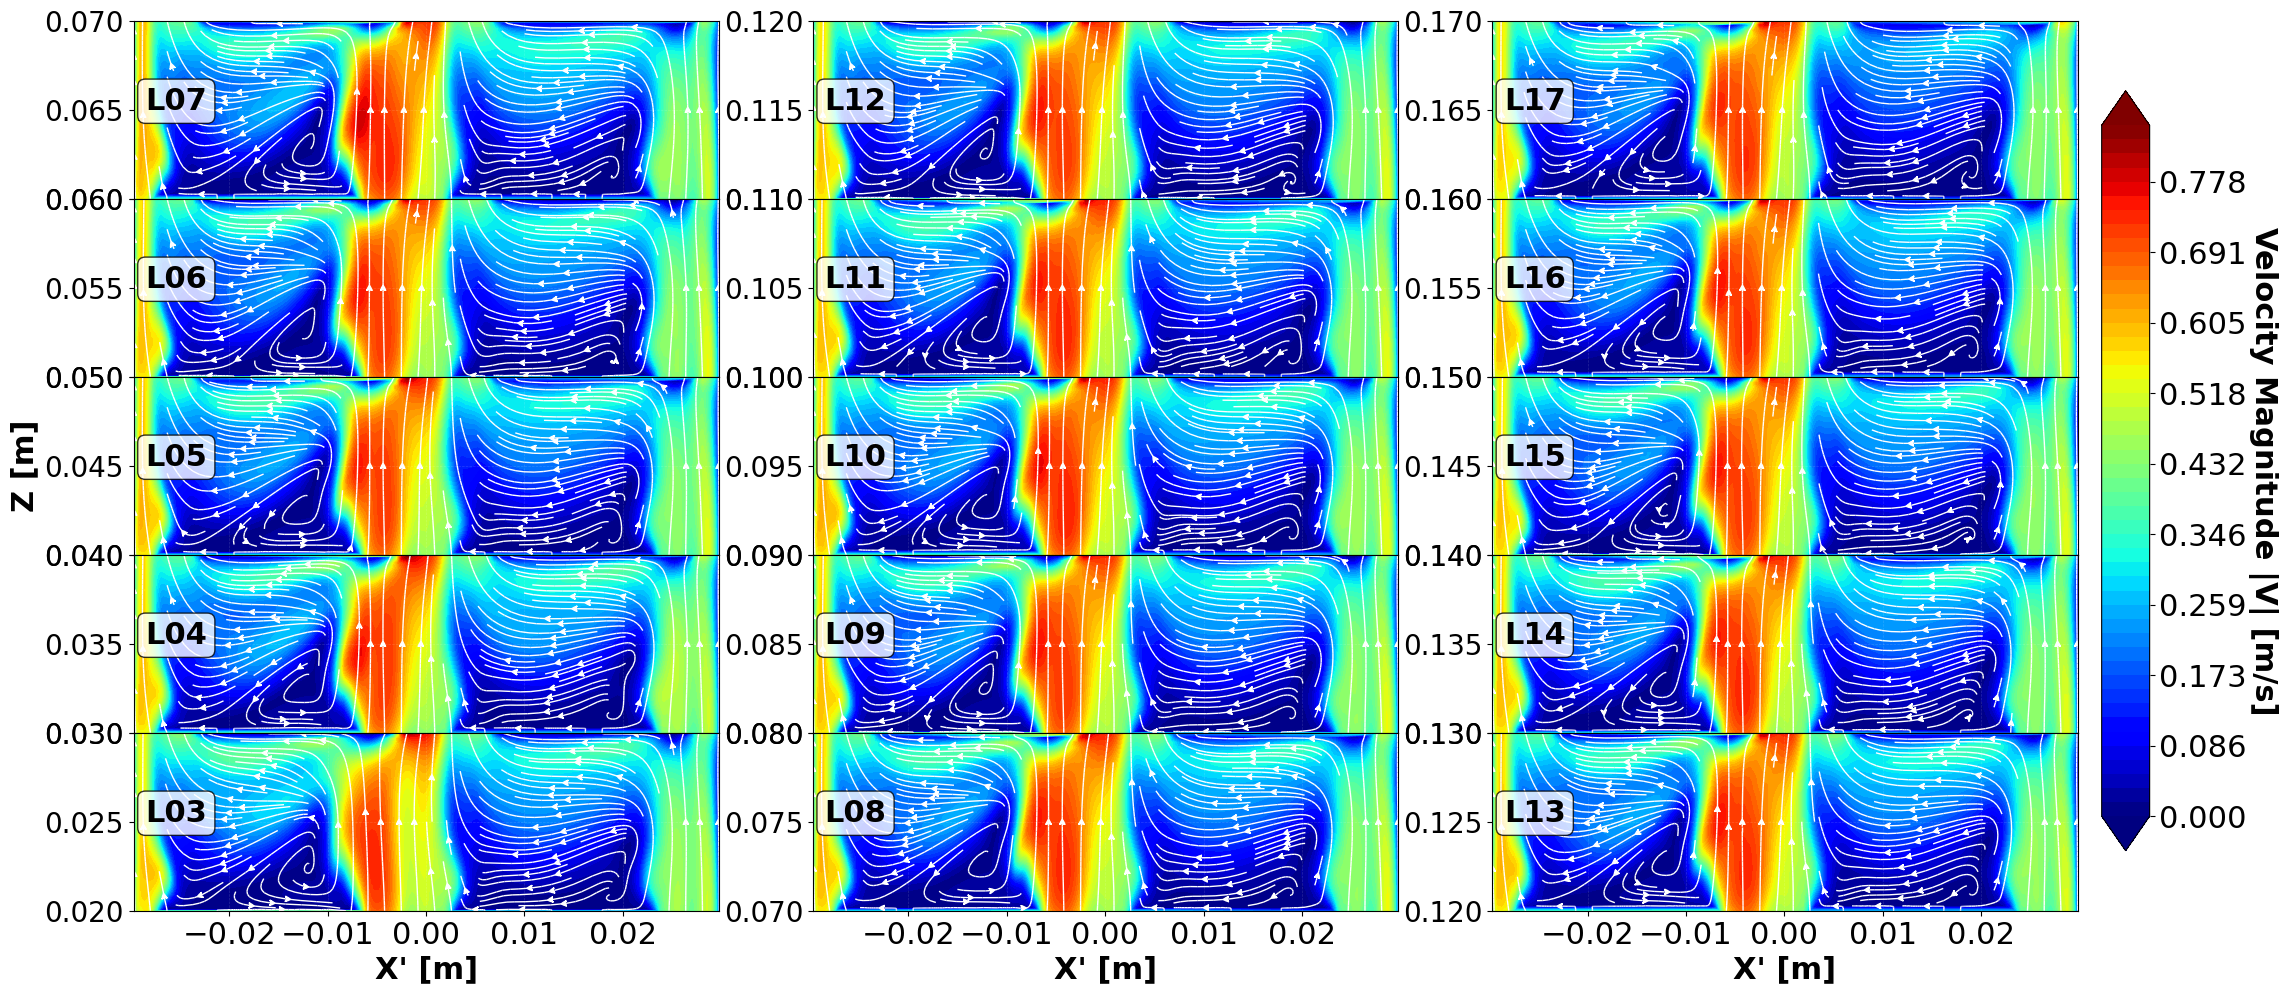
\includegraphics[width=0.78\linewidth]{30_Re_100/all_layers/Parallel_Sim_Velocity_Fields_Pos3_Re100_2col.png}
\caption{Results in the in-plane system for the time-averaged velocity magnitude obtained by LBM together with in-plane streamlines for all layers L03 to L17 of the packing with $\theta=30^\circ$ at Re$_p=100$. The periodic geometry produces a single repeating flow pattern across all developed layers, with noticeable differences observed only for L03, still impacted by the inflow condition.}
\label{fig:velocity_fields_30}
\end{figure}\begin{figure}[tbp]
\centering
\subfloat[$30^\circ$]{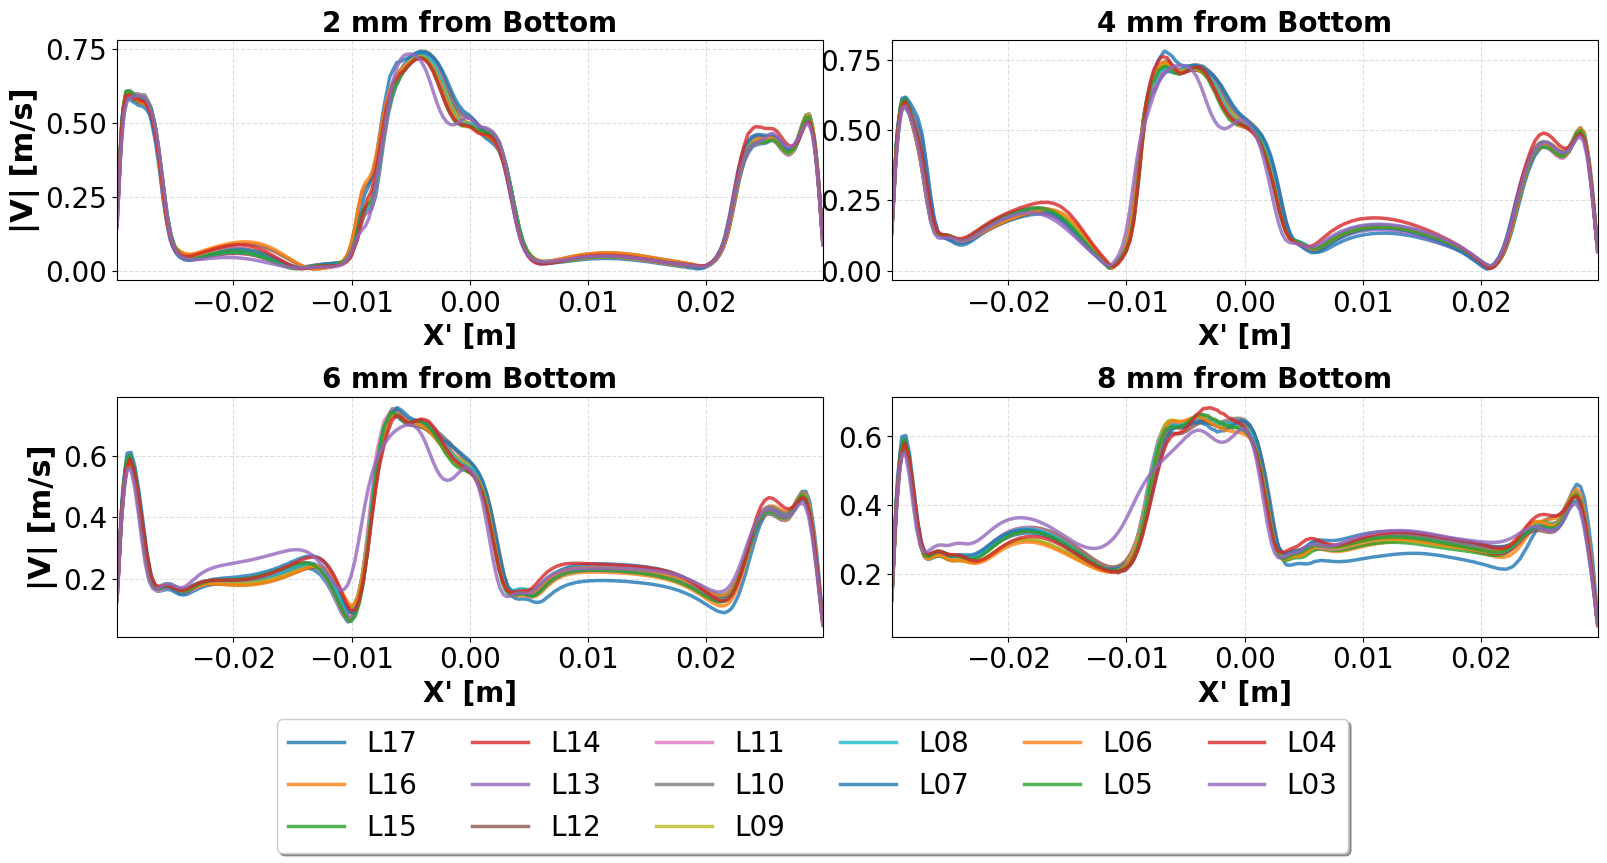
\includegraphics[width=0.72\linewidth]{images/30_Re_100/all_layers/Sim_Line_Profiles_from_Bottom_Pos3_Re100.png}}\\
\subfloat[$40^\circ$]{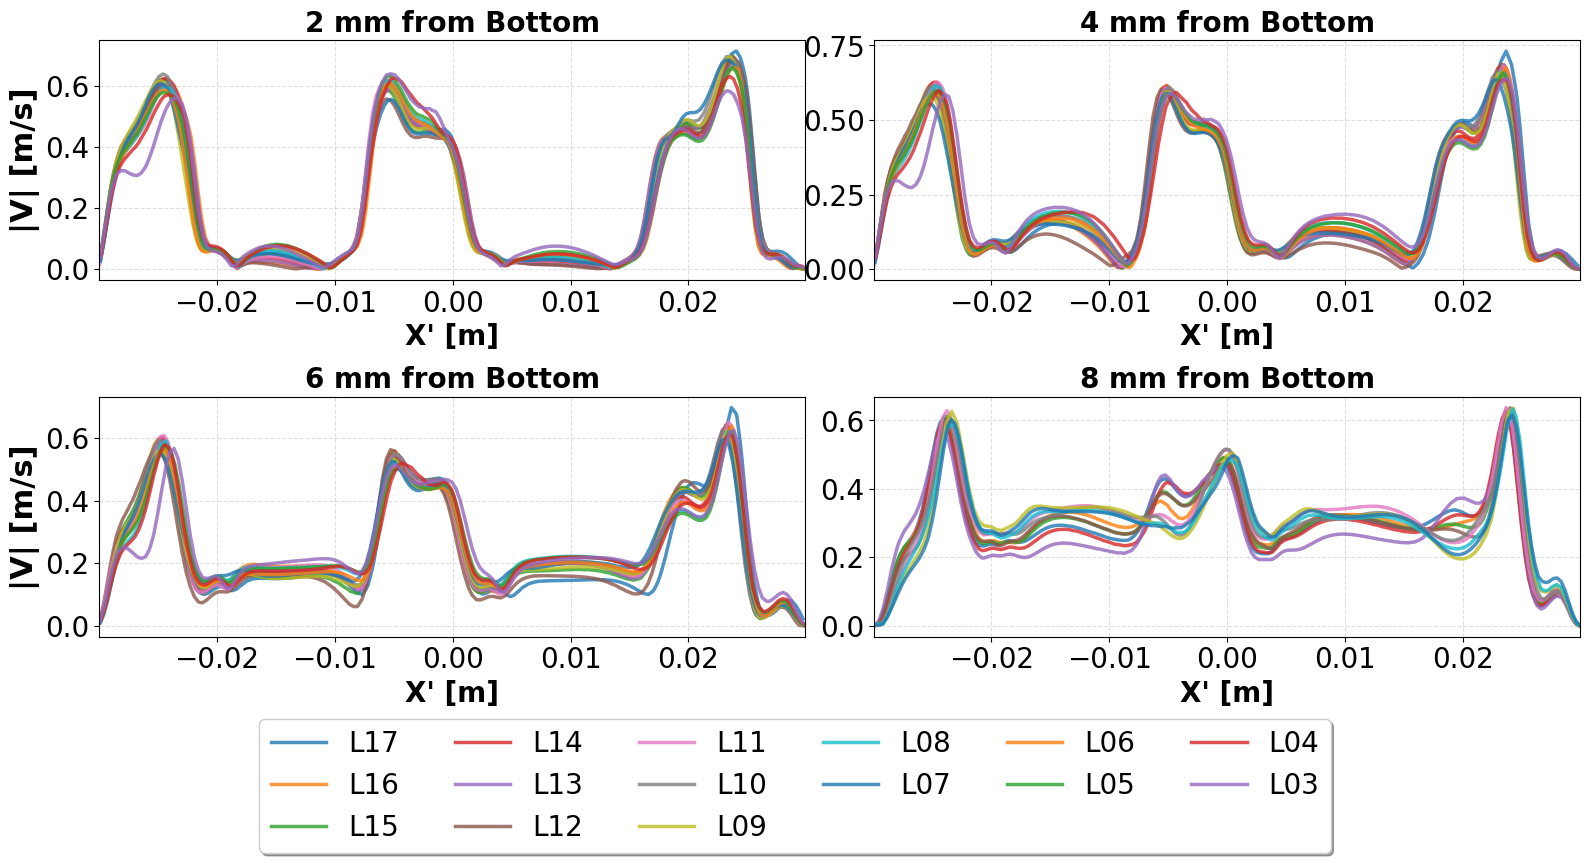
\includegraphics[width=0.72\linewidth]{images/40_Re_100/all_layers/Sim_Line_Profiles_from_Bottom_Pos3_Re100.png}}\\
\subfloat[Irregular]{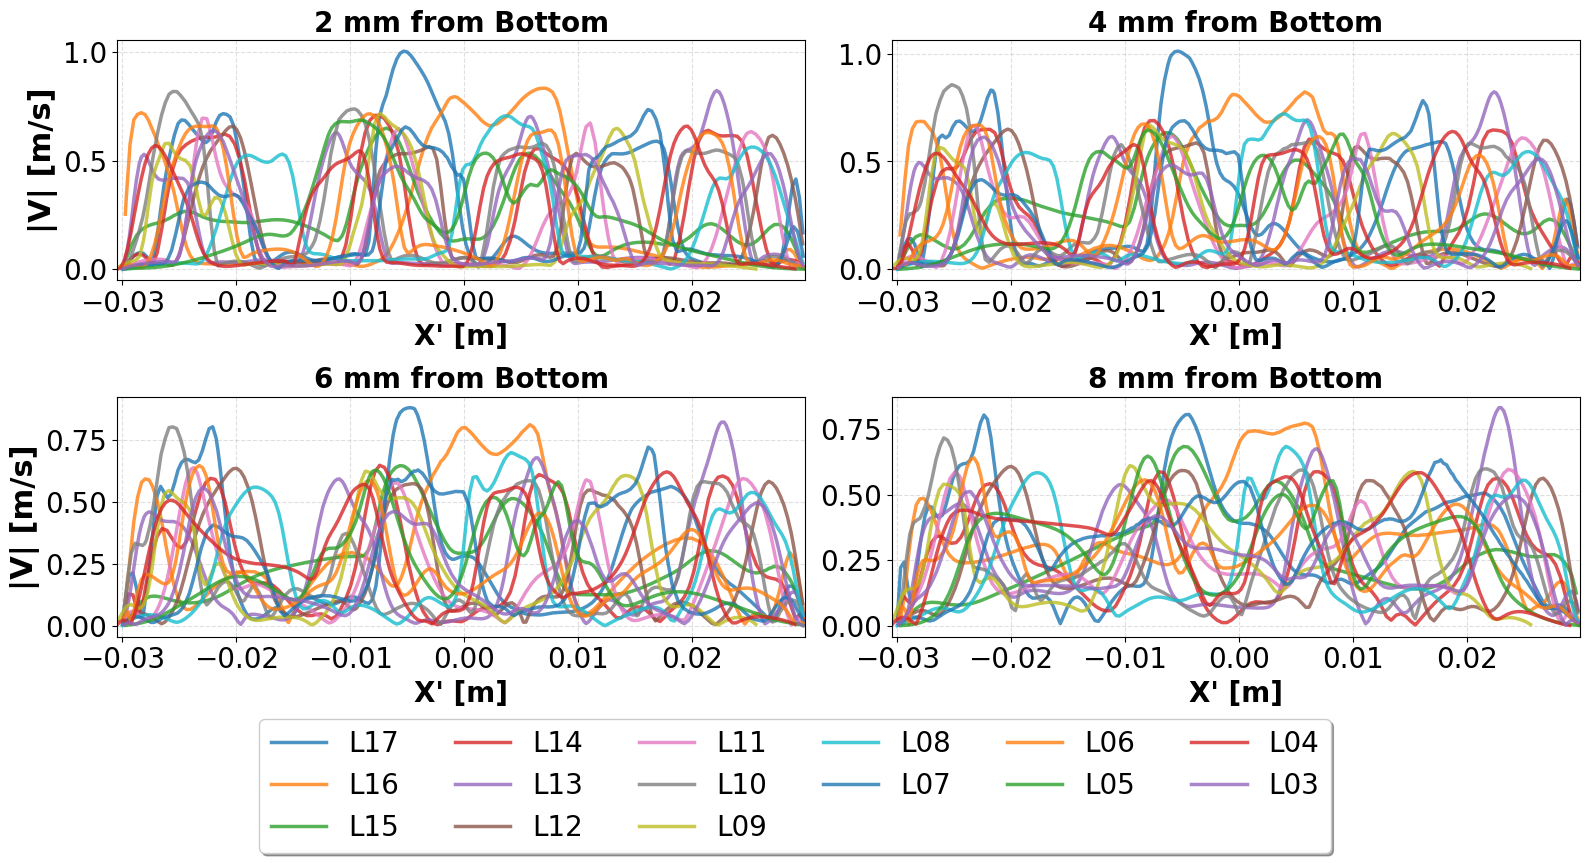
\includegraphics[width=0.72\linewidth]{images/irregular_Re_100/all_layers/Sim_Line_Profiles_from_Bottom_Pos3_Re100.png}}

\caption{Profiles of time-averaged velocity magnitude obtained by LBM at different heights within a module in each layer L03 to L17 at Pos3 for Re$_p=100$ in the topology (a)~$\theta=30^\circ$, (b)~$\theta=40^\circ$, and (c)~irregular packing. The periodic packings collapse mostly onto a common profile (though the first layer, L03, is still strongly impacted by the inflow condition), whereas the irregular packing exhibits very strong layer-to-layer variability throughout the whole bed.}
\label{fig:line_profiles_topology}
\end{figure}


\subsubsection{Flow Locking in Periodic and Irregular Packings}
\label{sec:locking:topologies}

Fig.~\ref{fig:Ln} shows the locking order parameter introduced in Section~\ref{sec:locking:Ln} for the periodic topologies at Re$_p = 100$ and for the irregular topology at Re$_p = 300$ in order to cover the extreme cases.\remark{17}{Since all six cases were simulated, I suggest showing the irregular case at Re$_p=100$ as the reference in Fig.~\ref{fig:Ln}(c), so that topology and Reynolds number are not confounded.} Supporting the discussion of Fig.~\ref{fig:velocity_fields_30}, in the in-plane system, the locking metric remains nearly constant across all fully developed layer pairs in the $30^\circ$ packing, with values approaching unity ($\overline{L}=0.998$). The negligible variation in the locking metric indicates that successive elements exhibit nearly identical pore-scale flow fields. This observation suggests that the time-averaged flow converges to a geometrically repeating state despite the relative complexity of the pore structure. The $40^\circ$ packing exhibits a similarly strong locking ($\overline{L}=0.993$) at this Reynolds number, demonstrating that this behaviour is a general consequence of \deleted{rotational periodicity}\added{a constant rotation angle} rather than a unique feature of a single topology. \added{Values close to unity are indeed expected from the screw symmetry of such stacks (Sec.~\ref{sec:geometry}) as long as the mean flow shares this symmetry; the informative content of the metric therefore lies mainly in the deviations from unity, caused, e.g., by the inlet region or by flow unsteadiness.}

The near-unity similarity values indicate that the rotational geometry repeatedly reorganises the flow into the same arrangement of jets and recirculation zones in each layer. Although individual jets accelerate, decelerate, and interact with bar wakes within a layer, the overall pore-scale transport pattern is reconstructed from one \deleted{geometrical period}\added{layer} to the next.

To verify that the observed locking originates from the packing topology rather than the comparison procedure, the same analysis was applied to the irregular configuration at Re$_p=300$. In contrast to the periodic packings, the layers now exhibit very little mutual similarity ($\overline{L}=0.46$), with each layer retaining distinct flow structures. The collapse observed for the periodic packings therefore arises from the \deleted{underlying rotational periodicity}\added{constant rotation angle} and not from the coordinate transformation or the similarity metric itself. The irregular packing thus provides a natural control that validates flow locking as a phenomenon genuinely induced by the \deleted{periodic geometry}\added{constant rotation angle}.

\begin{figure}[tbp]
\centering
\subfloat[$30^\circ$, Re$_p=100$]{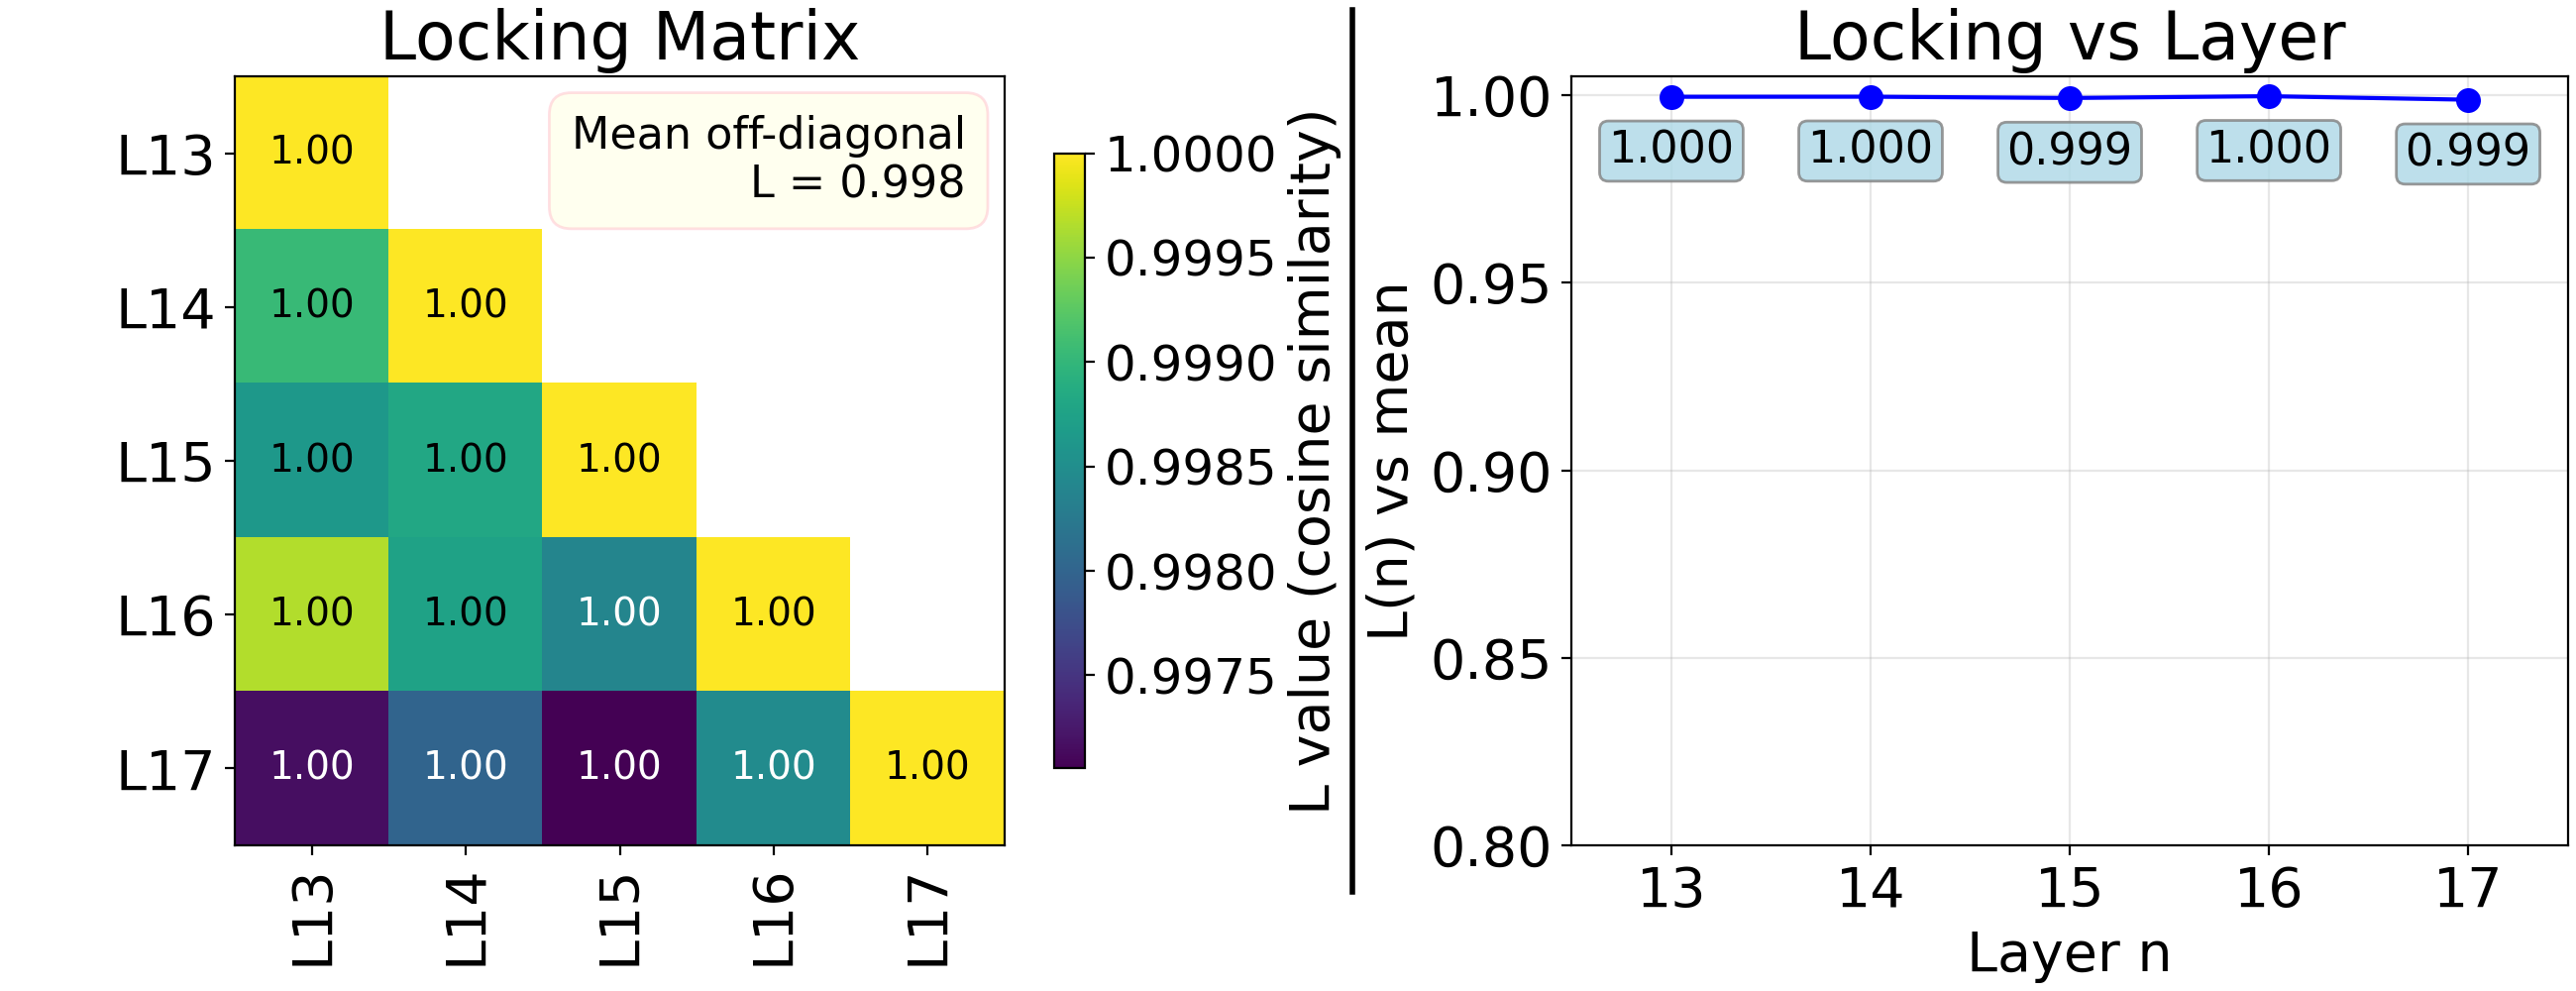
\includegraphics[width=0.85\linewidth]{Locking/Final_Ln_30_deg_Re=100_Pos3.png}}\\
\subfloat[$40^\circ$, Re$_p=100$]{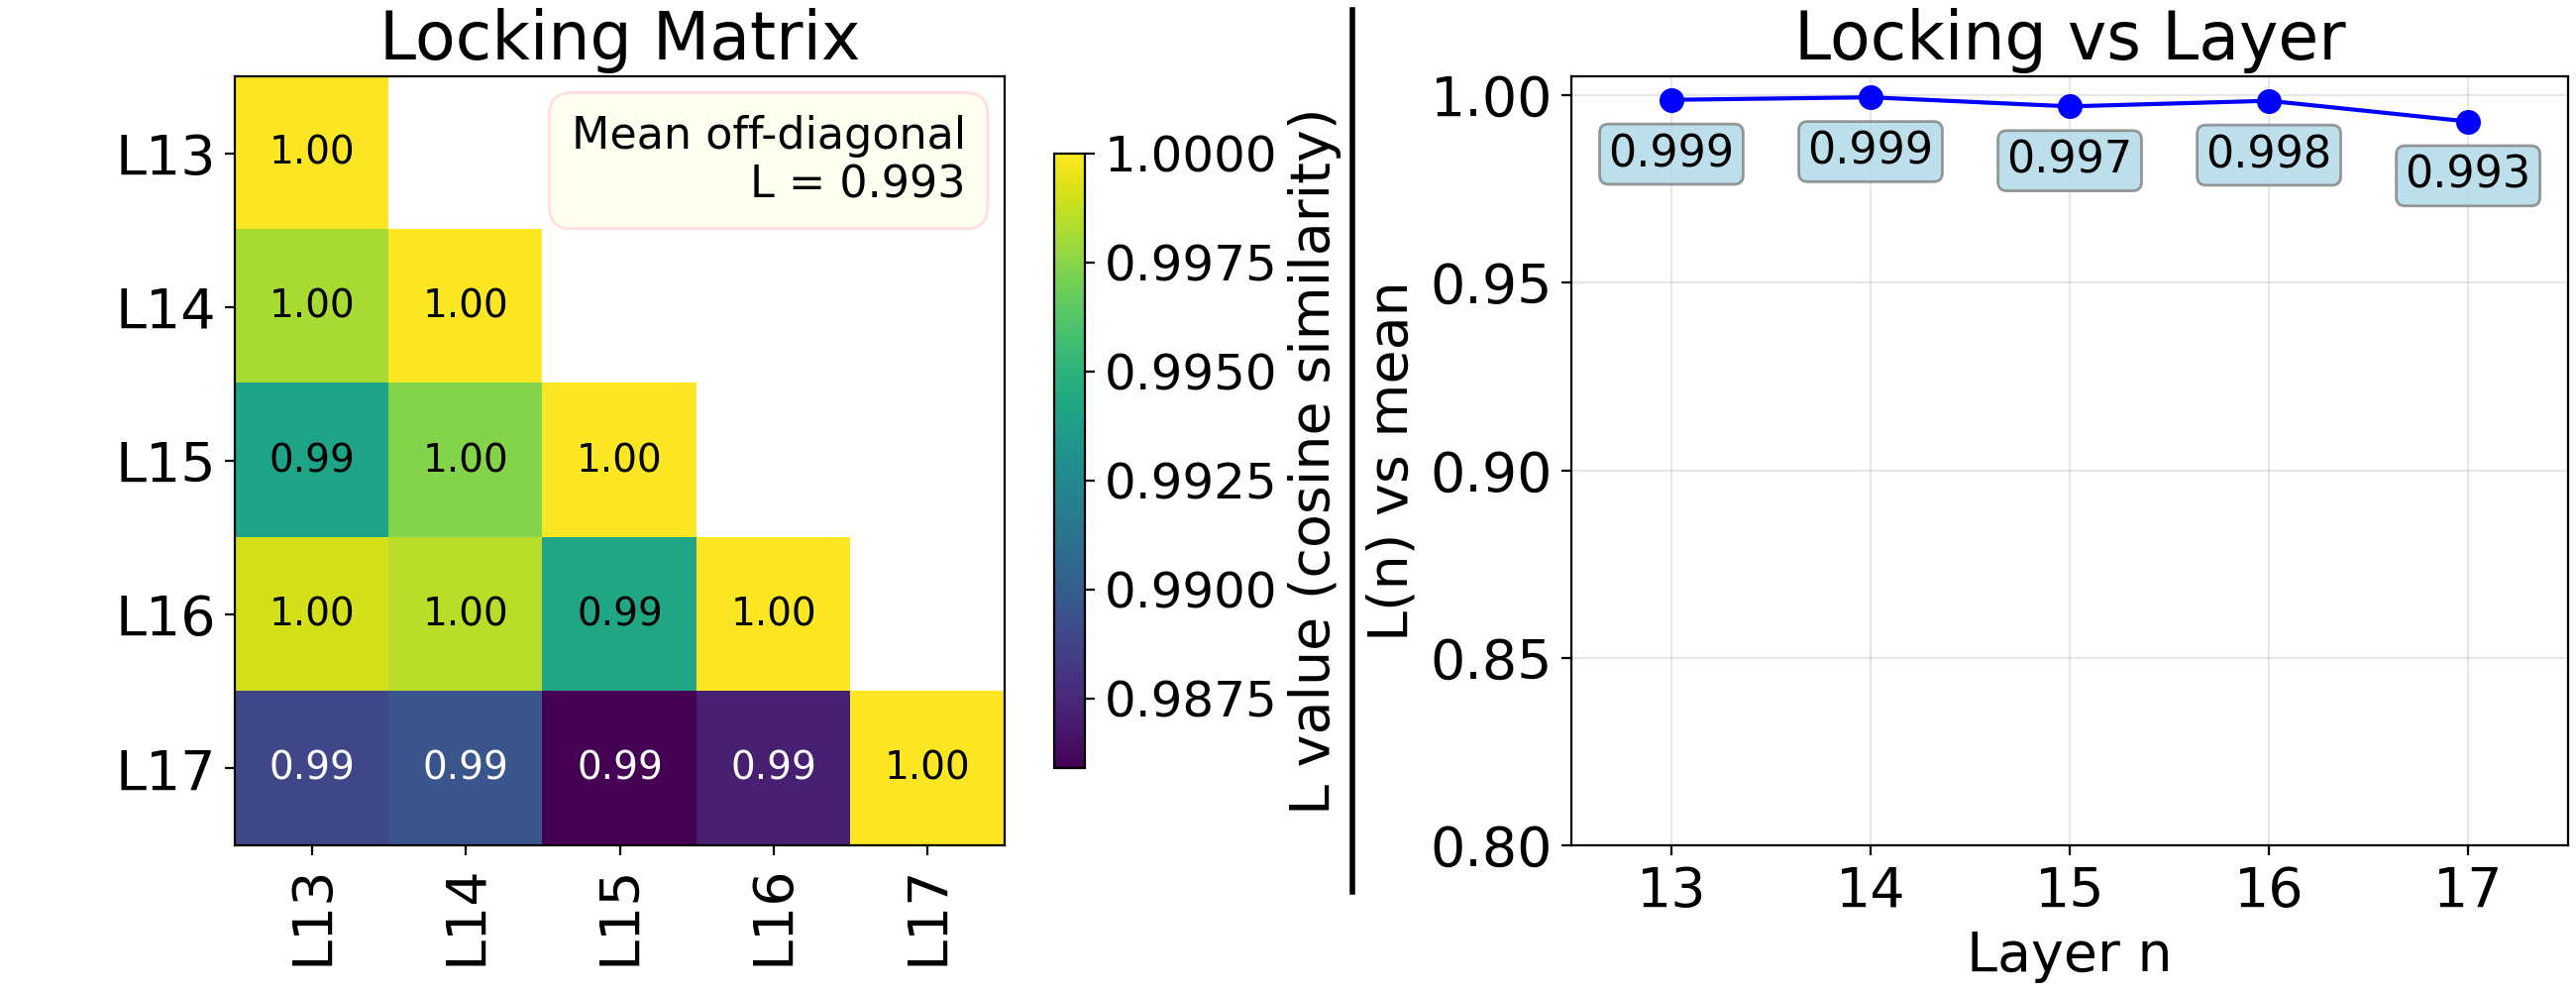
\includegraphics[width=0.85\linewidth]{Locking/Final_Ln_40_deg_Re=100_Pos3.png}}\\
\subfloat[irregular, Re$_p=300$]{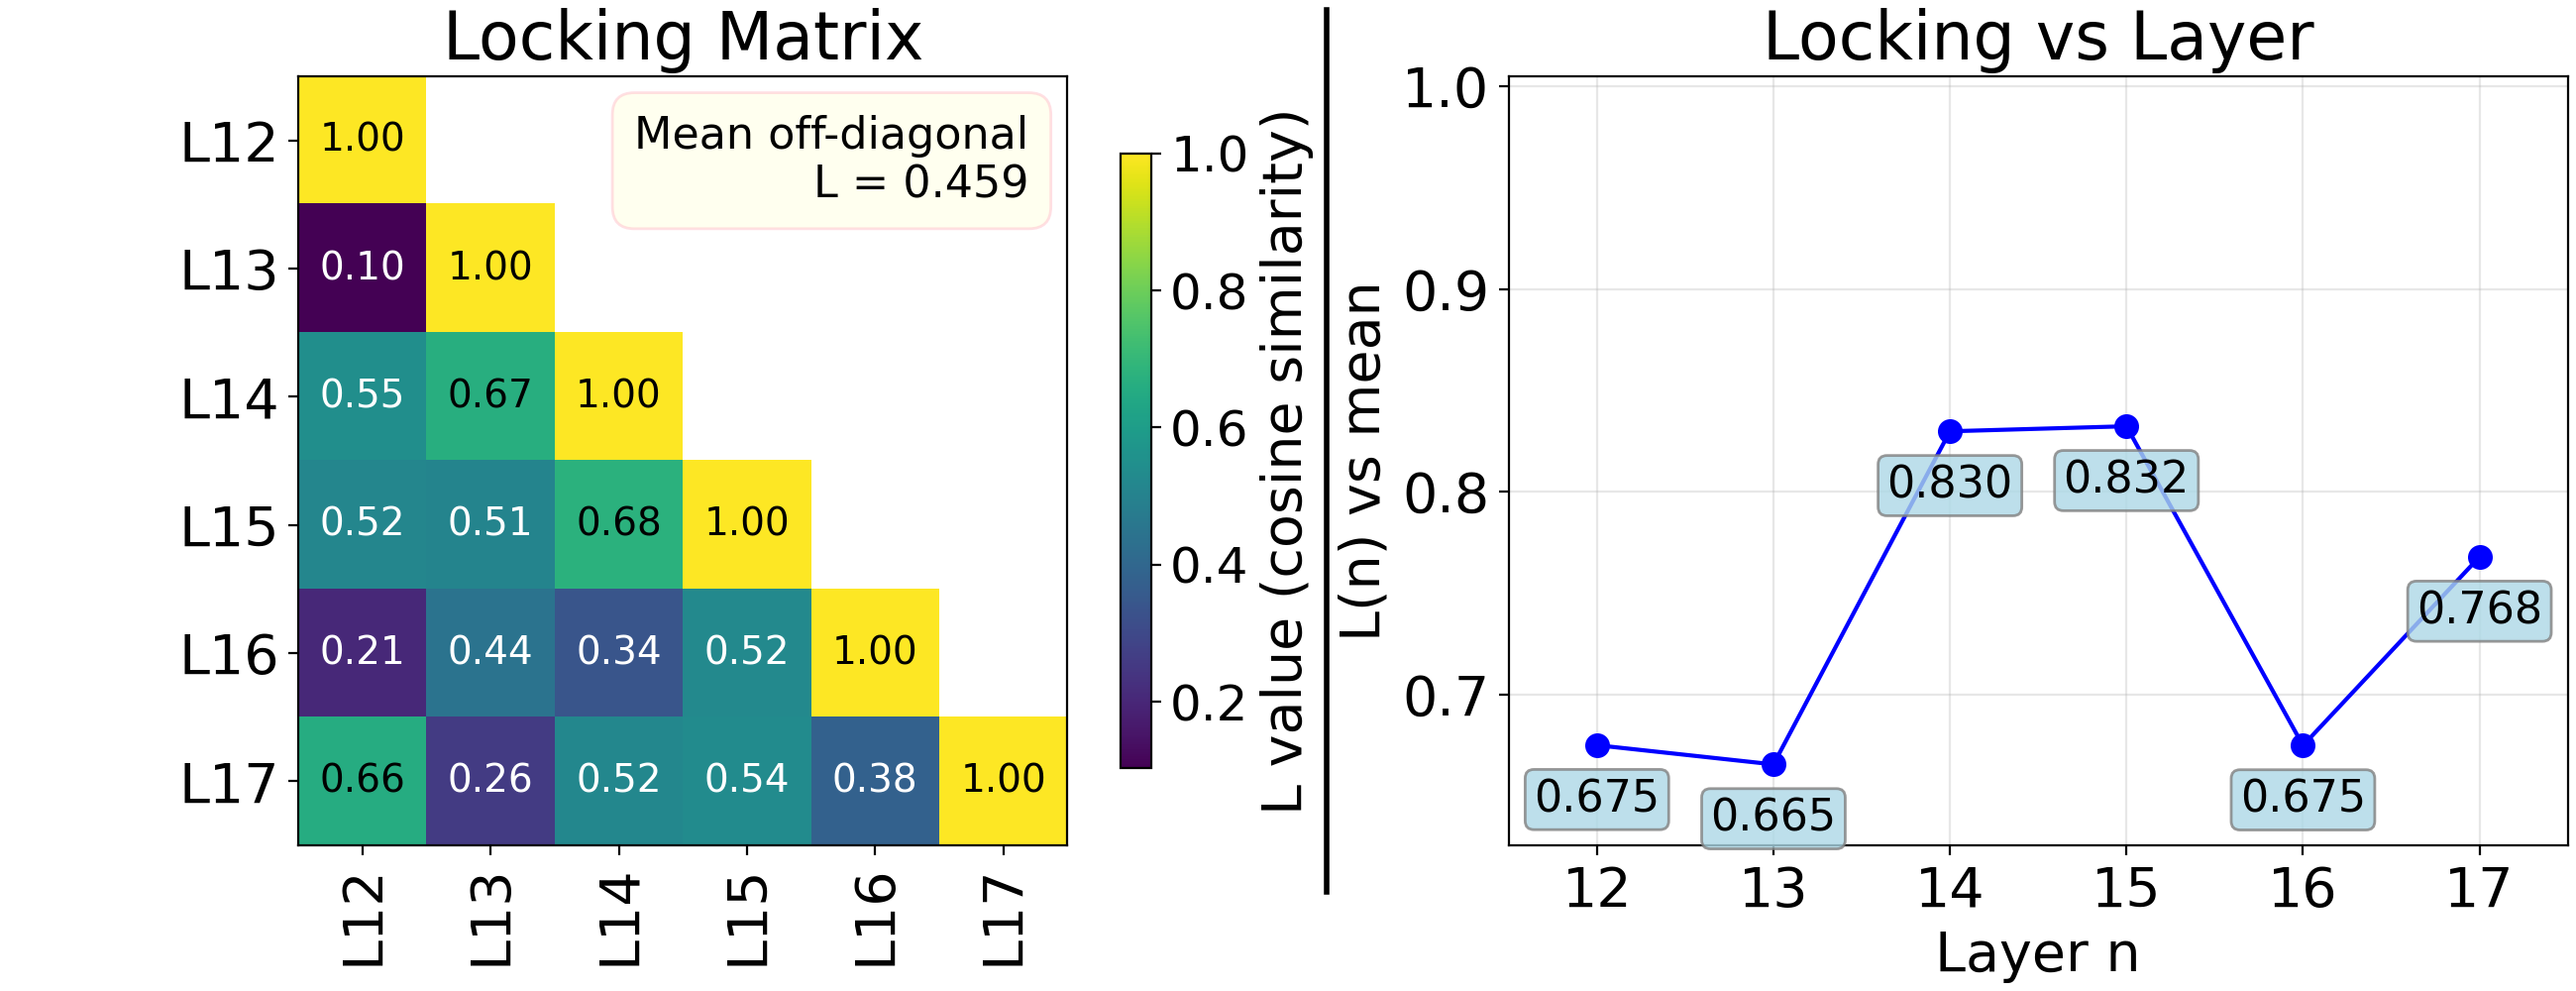
\includegraphics[width=0.85\linewidth]{Locking/Final_Ln_IR_deg_Re300_Pos3.png}}
\caption{Locking order parameter at Pos3 for the $30^\circ$ and $40^\circ$ packings at Re$_p = 100$ and for the irregular packing at Re$_p = 300$. Left: layer-to-layer matrix $L$ (Eq.~\ref{eq:Ln});
Right: per-layer locking $L(n)$ against the mean field involving all layers. The
(a)~$30^\circ$ and (b)~$40^\circ$ packings remain constant at $L \approx 1.00$ and $0.99$
respectively, whereas (c)~the irregular packing is much lower ($\overline{L}=0.46$, individual layer-pair values between $0.10$ and $0.68$,
$L(n)$ between $0.67$ and $0.83$), confirming that \deleted{the geometric period}\added{a constant rotation angle} is required for locking.}
\label{fig:Ln}
\end{figure}

\subsubsection{Flow Organisation}
\label{sec:organisation}

Having established the existence of flow locking, we now examine the details of the pore-scale flow structures responsible for this behaviour. In the in-plane system, the mean velocity fields collapse onto a repeating pattern consisting of high-velocity jets passing through the slit openings and recirculation zones in the wakes of the bars. These structures follow the layer-by-layer rotation of the packing and therefore trace spiral transport pathways through the bed. Specifically at Pos3, the flow is characterised by a dominant central jet flanked by two symmetric slit jets on both sides (Fig.~\ref{fig:velocity_fields_30}), a pattern that is reproduced throughout the developed region.

The two periodic packings organise the flow in slightly different ways. The $30^\circ$ packing exhibits \deleted{the most}\added{a highly} coherent structure, with well-defined slit jets and stable recirculation zones. Increasing the rotation angle to $40^\circ$ produces more inclined jets (see again Fig.~\ref{fig:validation_layers_40re100}) and enhanced transverse transport while preserving the overall periodic organisation. In contrast, the irregular packing loses this coherent structure: from one layer to the next, the number, position, width, and peak velocity of the jets as well as the size and location of the recirculation zones change (Fig.~\ref{fig:validation_layers_irreg}a; see also Fig.~\ref{fig:line_profiles_topology}c). This loss of coherent flow organisation explains the reduction in flow locking.

The two periodic topologies differ in the angle through which the flow must be redirected between successive layers. As the packing rotates by $\theta$, a jet leaving one slit must align with a differently oriented slit in the layer above. \deleted{For the $30^\circ$ packing, this redirection is relatively small, which helps to preserve the jet structure from layer to layer ($\overline{L}=0.998$). Increasing the rotation to $40^\circ$ requires stronger transverse momentum redistribution, producing stronger inter-layer shear layers.} At Re$_p=100$, the flow \deleted{nevertheless remains}\added{remains} highly organised \added{in both cases} ($\overline{L}=0.998$ \added{and $0.993$}), and the small difference with respect to the $30^\circ$ packing ($0.005$) is too small for any ranking of the two angles to be inferred.\remark{18}{The mechanistic explanation for a higher coherence at $30^\circ$ was removed, since the difference is declared too small for a ranking and the order reverses at Re$_p=300$.}

These findings show that flow locking is a consequence of \deleted{rotational periodicity}\added{a constant rotation angle}, whereas the exact value of the rotation angle plays only a minor role between the two periodic angles considered. A strongly locked flow preserves coherent transport pathways through successive layers, leading to predictable local residence times and interstitial transport. In the irregular packing, by contrast, no such layer-to-layer repeatability can be expected.

\subsubsection{Impact of Reynolds Number}
\label{sec:locking:reynolds}

To investigate the influence of the Reynolds number, the analysis is repeated at Re$_p=300$ for the two periodic topologies (Fig.~\ref{fig:Ln_re300}). Both periodic packings remain strongly locked, with $\overline{L}=0.973$ for $30^\circ$ and $\overline{L}=0.981$ for $40^\circ$, compared with $0.998$ and $0.993$ at Re$_p=100$. Increasing the Reynolds number therefore weakens flow locking only slightly (by $0.025$ and $0.012$, respectively). A likely reason is that the flow inside the packing becomes slightly unsteady at Re$_p=300$ (Section~\ref{sec:validation:layers}). These slow oscillations do not average out completely, so the mean field of each layer keeps a small imprint that differs from one layer to the next. In addition, the jets and wakes carry more inertia at higher Reynolds numbers and follow the local slit geometry a little less strictly, so each layer is somewhat more affected by its neighbours. The difference between the two angles at Re$_p=300$ is about as large as the layer-to-layer scatter, so we do not rank the two topologies here.

\begin{figure}[tbp]
\centering
\subfloat[$30^\circ$, Re$_p=300$]{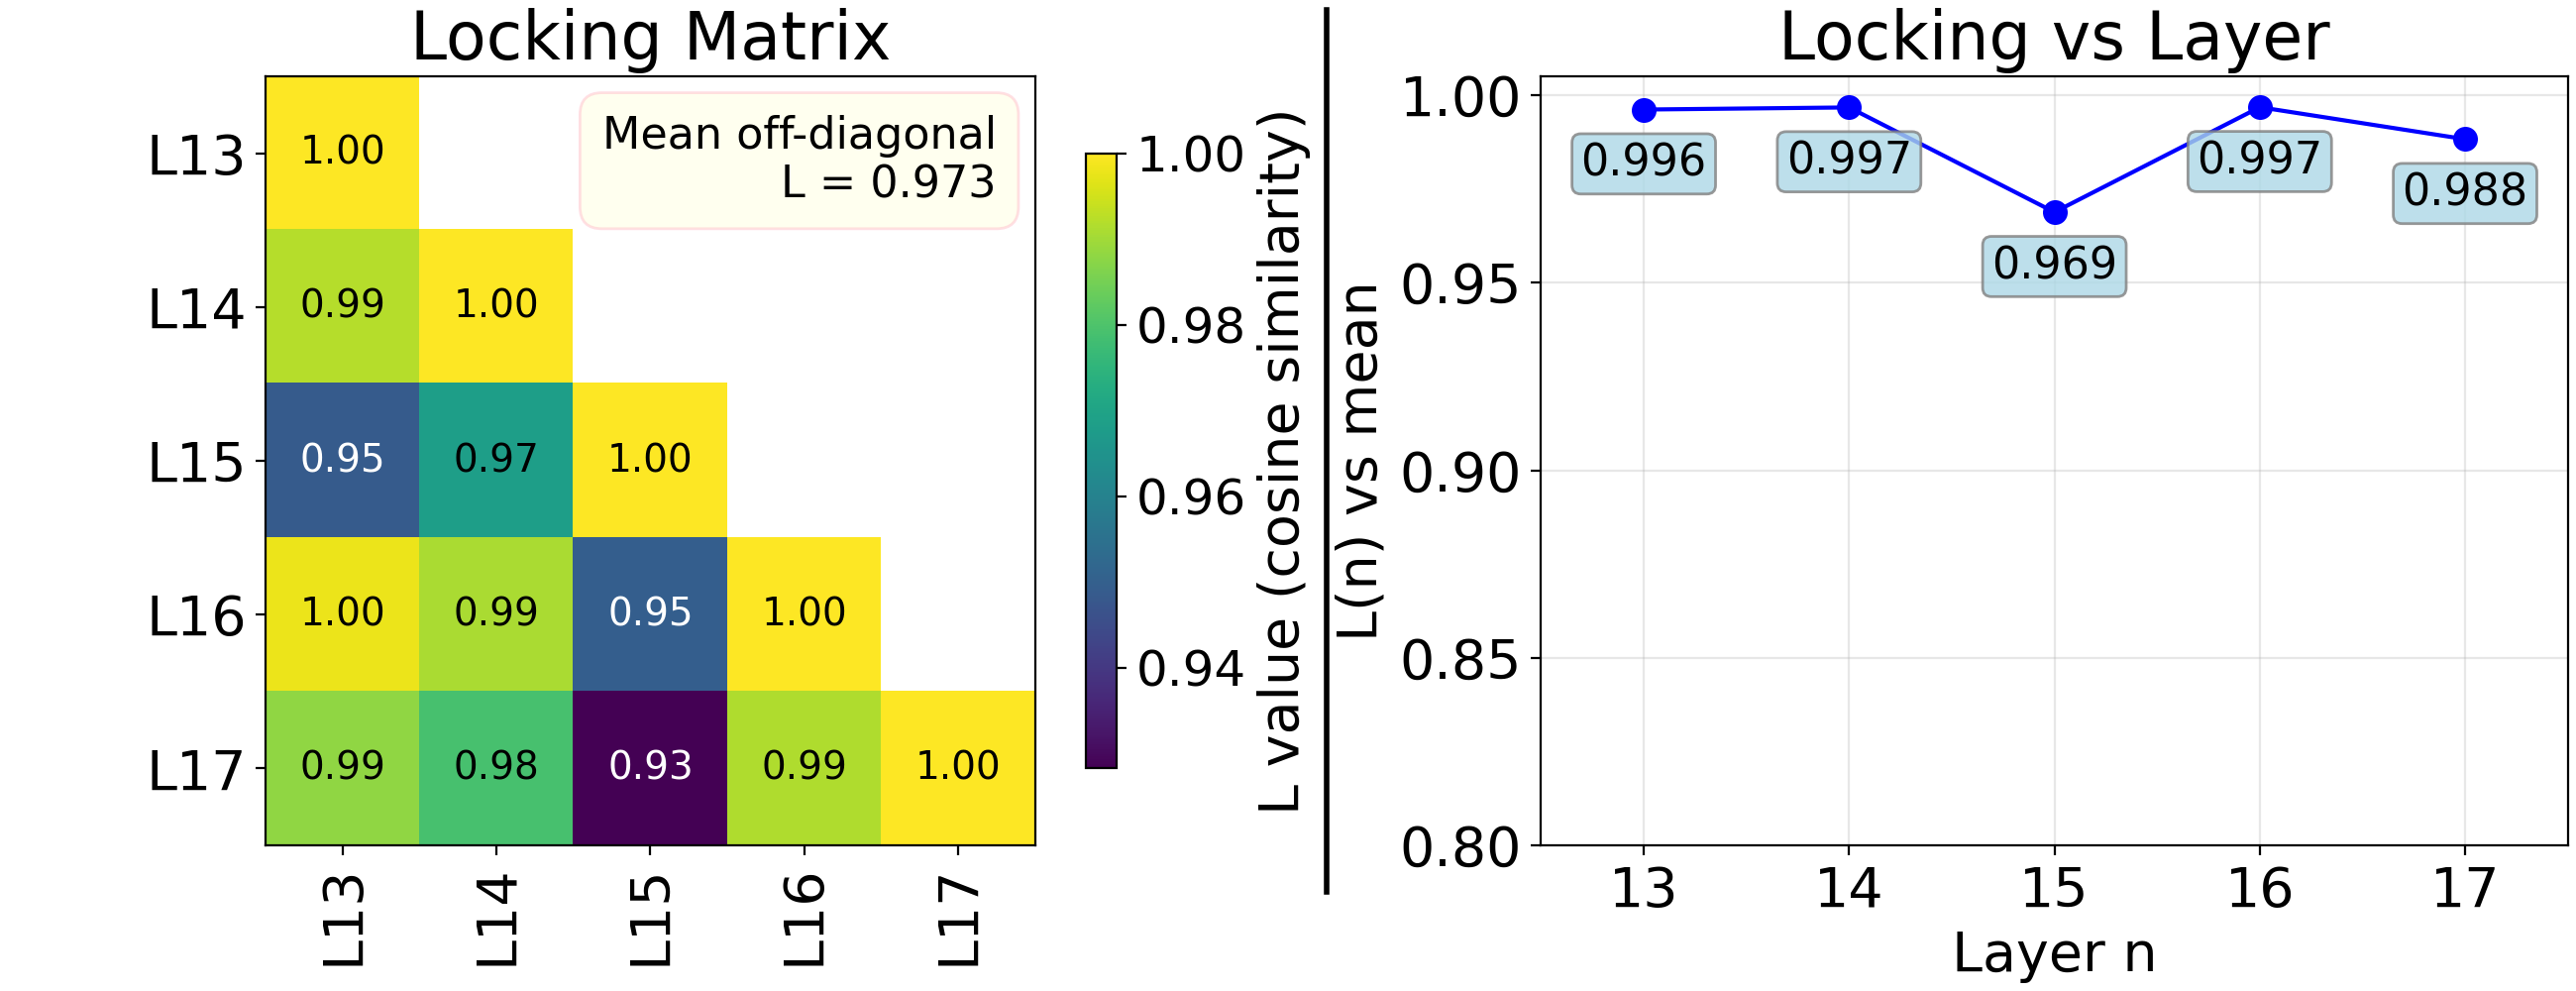
\includegraphics[width=0.85\linewidth]{Locking/Final_Ln_30_deg_Re300_Pos3.png}}\\
\subfloat[$40^\circ$, Re$_p=300$]{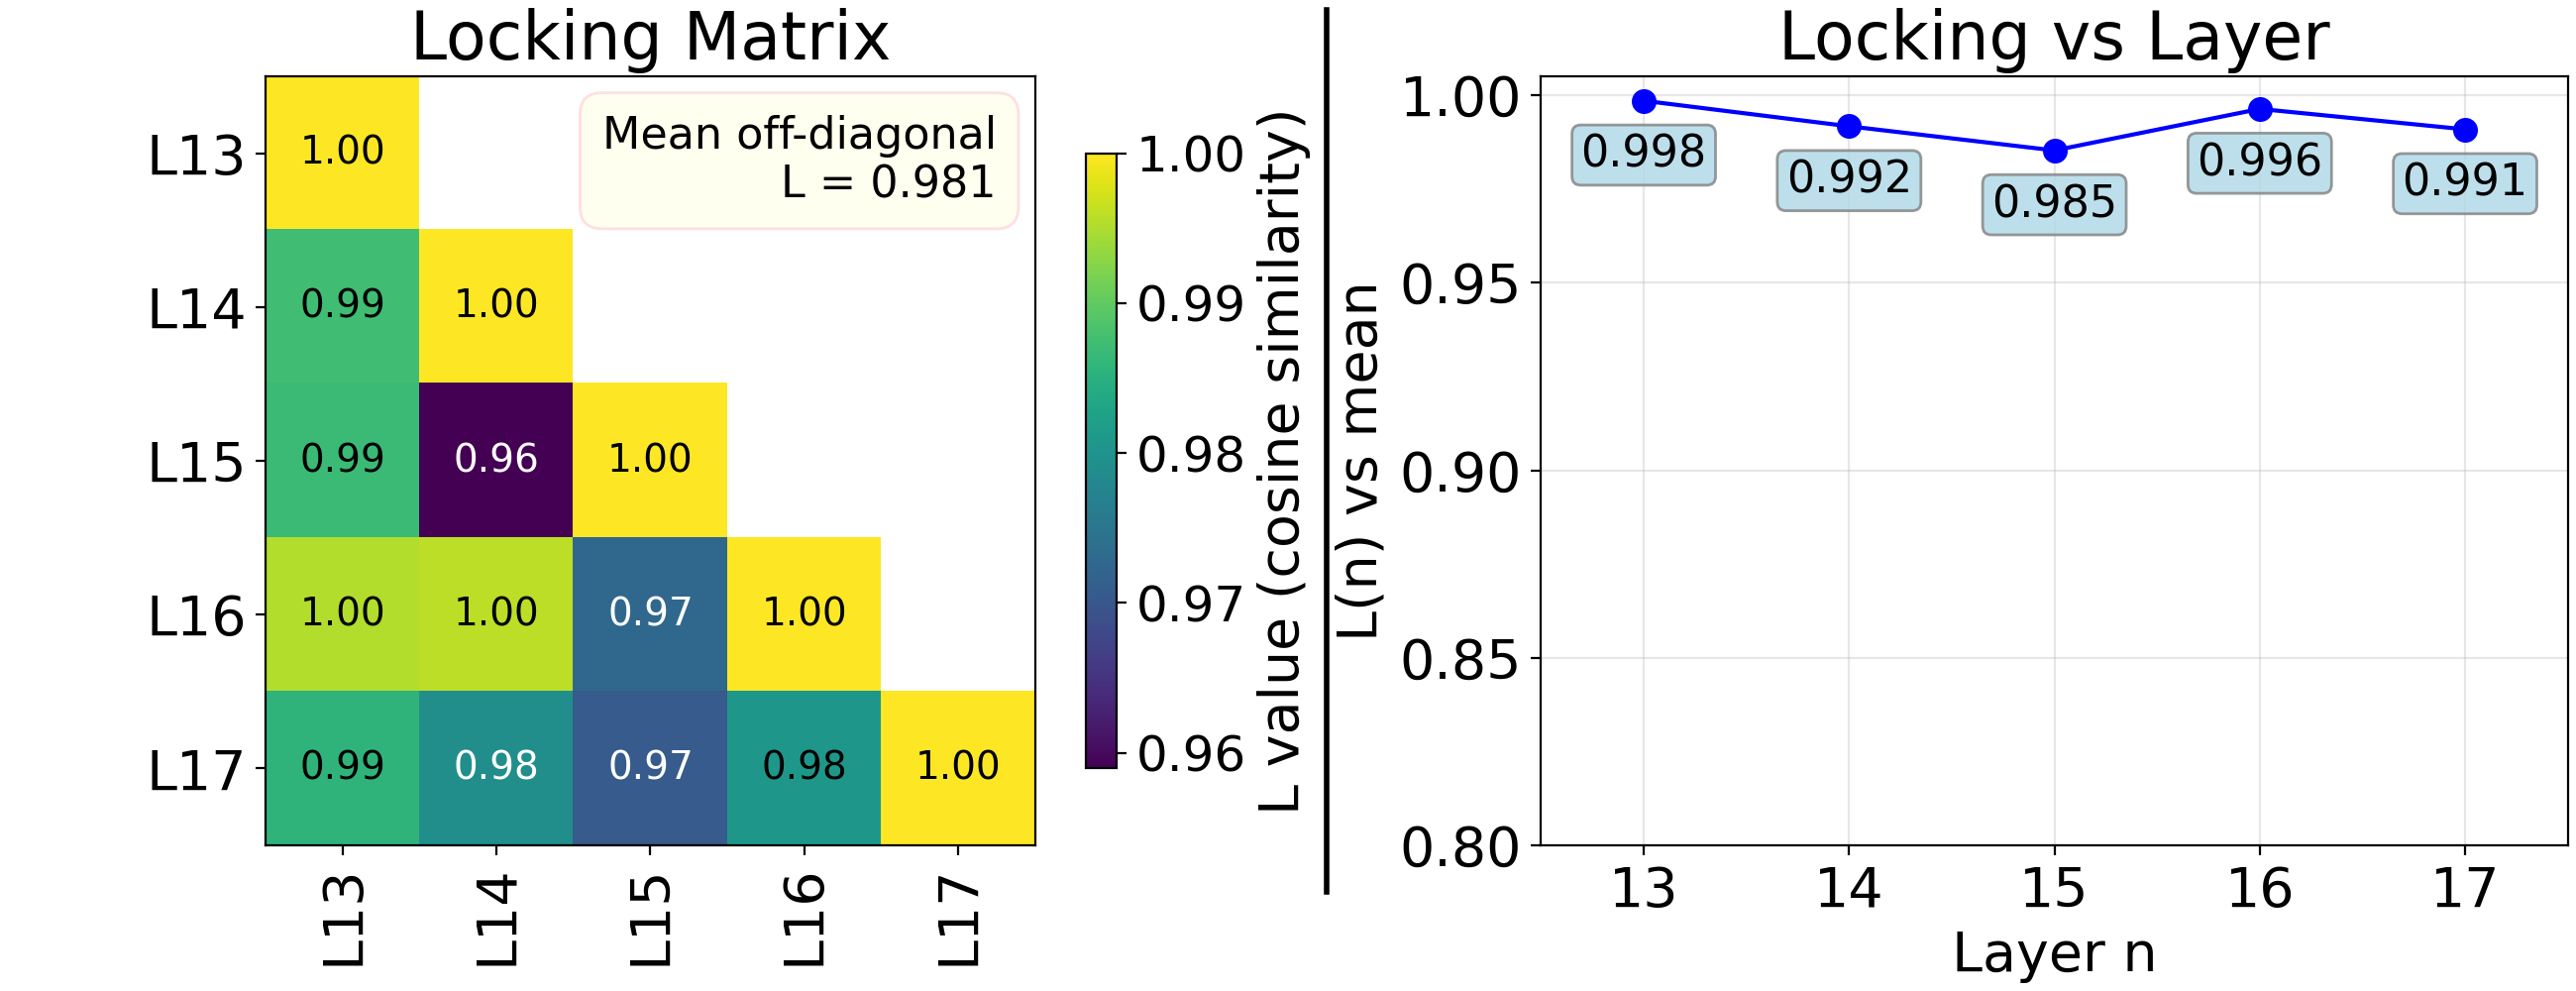
\includegraphics[width=0.85\linewidth]{Locking/Final_Ln_40_deg_Re300_Pos3.png}}
\caption{Locking metric at Re$_p=300$ for the (a) $30^\circ$ and (b) $40^\circ$ periodic packings. Both packings remain strongly locked ($\overline{L}=0.973$ at $30^\circ$, $\overline{L}=0.981$ at $40^\circ$), but at a slightly lower level than at Re$_p=100$ ($\overline{L}=0.998$ and $0.993$).}

\label{fig:Ln_re300}
\end{figure}

Part of the decrease may also come from the finite averaging time at Re$_p=300$. This is only a tentative interpretation, and longer averaging would be needed to confirm it.

Over the range of Reynolds numbers considered here, the periodic packings thus remain strongly locked. Higher Reynolds numbers have not been numerically investigated yet.

\section{Conclusions}

A central-moment lattice Boltzmann solver was used to study the gas flow in a model packed bed made of identical elements stacked with a prescribed rotation between successive layers. Three topologies were considered: two rotationally periodic packings ($\theta=30^\circ$ and $40^\circ$) and one irregular packing, at particle Reynolds numbers Re$_p=100$ and $300$. After a grid-convergence analysis, %based on three resolutions showed that the medium grid is sufficient at Re$_p=100$, with a discretisation uncertainty below $1\%$ on the fine grid for the mean velocity.
the simulations were validated against planar PIV measurements, both in the freeboard above the bed and within individual layers. For the $30^\circ$ packing, the agreement in the freeboard corresponds to $\mathrm{NRMSE}=6\%$ and $R^2=0.92$ at Re$_p=100$, and $\mathrm{NRMSE}=5\%$ and $R^2=0.95$ at Re$_p=300$. Jet positions, widths and recirculation zones are also reproduced in the individual layers of the $40^\circ$ and irregular packings. The remaining differences are located mostly in the thin shear layers bordering the jets, where \deleted{the numerical dissipation of the second-order scheme may slightly smooth narrow velocity peaks; finer grids or a higher-order discretisation would be expected to reduce them}\added{the measured velocity fluctuations are also strongest}.

On this basis, the recurrence of the time-averaged pore-scale flow from layer to layer (flow locking) was quantified with a similarity metric applied to the velocity fields in the in-plane system. In both periodic packings the flow is almost identical in successive layers at Re$_p=100$ ($\overline{L}=0.998$ for $30^\circ$ and $0.993$ for $40^\circ$), whereas the irregular packing shows little similarity ($\overline{L}=0.46$ at Re$_p=300$). At Re$_p=300$, both periodic packings remain strongly locked. Because the flow repeats \deleted{over each geometric period}\added{from layer to layer for a constant rotation angle}, a single periodic module \added{(or even a single layer with rotate-and-shift periodic boundary conditions)} can represent the developed region of such a bed, and the metric offers a way to check this assumption quantitatively.

Up to now, only two rotation angles, one irregular packing and two Reynolds numbers were considered numerically, and the study concerns a model packed bed designed specifically for validation purposes. Additional angles and Reynolds numbers will be considered to establish the range over which flow locking occurs, and an extension to scalar transport will show whether the recurrence of the flow also applies to mixing and heat or mass transfer.

\begin{acknowledgments}
This work was funded by the Deutsche Forschungsgemeinschaft (DFG, German Research Foundation) - Project-ID 422037413 - TRR 287. The simulations were carried out on the Sofja cluster of the Otto von Guericke University Magdeburg.
The experimental equipment was funded by the German Research foundation Project-ID 279416000.
\end{acknowledgments}

\section*{Declarations}
\textbf{Conflict of interest} The authors declare that they have no conflict of interest.\\
\textbf{Data availability} The experimental data for the 40° configuration is available under ReSeeD Research Data Repository, (https://doi.org/10.60517/cn69m9200). The data supporting the findings of this study are available from the corresponding author upon reasonable request.

% For one-column wide figures use
%\begin{figure}
% Use the relevant command to insert your figure file.
% For example, with the graphicx package use
%  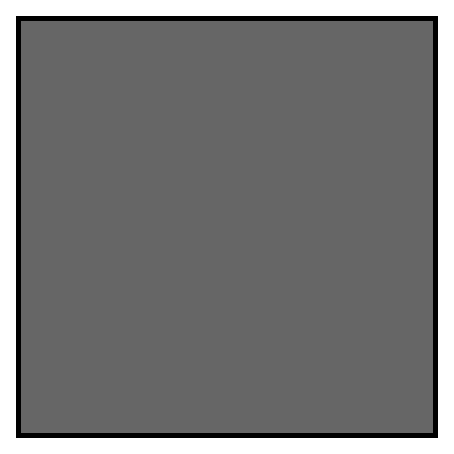
\includegraphics{example.eps}
% figure caption is below the figure
%\caption{Please write your figure caption here}
%\label{fig:1}       % Give a unique label
%\end{figure}
%
% For two-column wide figures use
%\begin{figure*}
% Use the relevant command to insert your figure file.
% For example, with the graphicx package use
%  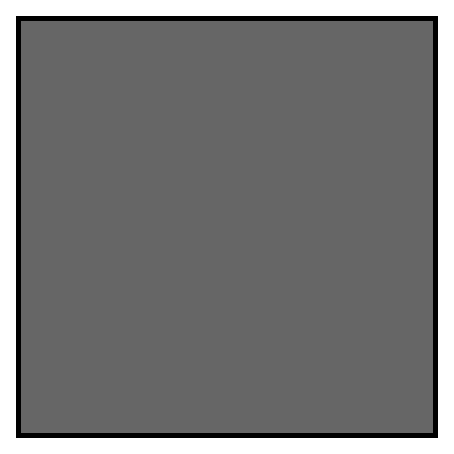
\includegraphics[width=0.75\textwidth]{example.eps}
% figure caption is below the figure
%\caption{Please write your figure caption here}
%\label{fig:2}       % Give a unique label
%\end{figure*}
%
% For tables use
%\begin{table}
% table caption is above the table
%\caption{Please write your table caption here}
%\label{tab:1}       % Give a unique label
% For LaTeX tables use
%\begin{tabular}{lll}
%\hline\noalign{\smallskip}
%first & second & third  \\
%\noalign{\smallskip}\hline\noalign{\smallskip}
%number & number & number \\
%number & number & number \\
%\noalign{\smallskip}\hline
%\end{tabular}
%\end{table}


%\begin{acknowledgements}
%If you'd like to thank anyone, place your comments here
%and remove the percent signs.
%\end{acknowledgements}

% BibTeX users please use one of
%\bibliographystyle{spbasic}      % basic style, author-year citations
%\bibliographystyle{spmpsci}      % mathematics and physical sciences
%\bibliographystyle{spphys}
%  - tighten vertical space around figures  -
\setlength{\intextsep}{4pt plus 2pt minus 2pt}     % space above/below in-text ([H]/here) floats
\setlength{\textfloatsep}{6pt plus 2pt minus 2pt}  % space between top/bottom floats and text
\setlength{\abovecaptionskip}{4pt}                 % image-to-caption gap
\setlength{\belowcaptionskip}{0pt}
%
% and use \bibitem to create references. Consult the Instructions
% for authors for reference list style.
%
%\bibitem{RefJ}
% Format for Journal Reference
%Author, Article title, Journal, Volume, page numbers (year)

%% ============================================================
%\bibliography{references}
\bibliography{references_2026_11_18_fv}

\end{document}
